\documentclass[11pt,twoside,english,singlespacing,headsepline,consistentlayout]{auxiliary/si-msc-thesis}

\usepackage[utf8]{inputenc} % Required for inputting international characters
\usepackage[T1]{fontenc} % Output font encoding for international characters

\usepackage{lipsum}
\usepackage{mathpazo}
\usepackage{float}
\usepackage{makecell}
\usepackage{listings}
\usepackage{cite}
\usepackage{zlmtt}
\usepackage{fancyvrb}
\usepackage{algorithm}
\usepackage{algpseudocode}
\usepackage{subcaption}
\usepackage{tabularx}
\usepackage{amssymb}
\usepackage{pifont}
\usepackage{rest-api}
\usepackage{afterpage}
\usepackage{amsmath}
\usepackage{simplebnf}

\newcommand\blankpage{%
    \null
    \thispagestyle{empty}%
    \addtocounter{page}{-1}%
    \newpage}

\colorlet{darkgreen}{green!70!black}
\colorlet{darkred}{red!70!black}
\colorlet{punct}{red!60!black}
\definecolor{delim}{RGB}{20,105,176}
\definecolor{eclipseKeywords}{RGB}{127,0,85}

\newcommand\jsonkey{\color{red}}
\newcommand\jsonvalue{\color{teal}}
\newcommand\jsonnumber{\color{black}}
\newcommand\YAMLcolonstyle{\color{black}}
\newcommand\YAMLkeystyle{\color{red}}
\newcommand\YAMLvaluestyle{\color{teal}}

% here is a macro expanding to the name of the language
% (handy if you decide to change it further down the road)
\lstdefinelanguage{yaml}{
    basicstyle=\YAMLkeystyle,                                 % assuming a key comes first
    sensitive=false,
    comment=[l]{\#},
    morecomment=[s]{/*}{*/},
    commentstyle=\YAMLkeystyle,
    stringstyle=\YAMLvaluestyle,
    moredelim=**[il][\YAMLcolonstyle{:}\YAMLvaluestyle]{:},   % switch to value style at :
    morestring=[b]',
    morestring=[b]",
    basicstyle=\ttfamily
}

\lstdefinelanguage{docker}{
    keywords={FROM, RUN, COPY, ADD, ENTRYPOINT, ENV, ARG, WORKDIR, EXPOSE, LABEL, USER, VOLUME, STOPSIGNAL, ONBUILD, MAINTAINER},
    keywordstyle=\color{blue},
    identifierstyle=\color{black},
    sensitive=false,
    comment=[l]{\#},
    commentstyle=\color{darkgray},
    stringstyle=\color{teal},
    morestring=[b]',
    morestring=[b]",
    basicstyle=\ttfamily
}

\lstset{language=docker, literate={ü}{{\"u}}1 {-}{-}1, showstringspaces=false}

\lstdefinelanguage{docker-compose}{
    keywords={version, volumes, services, image, environment, ports, container_name, ports, links, build, networks, mongo_db, es_db, external, models_ct},
    keywordstyle=\color{black},
    identifierstyle=\color{teal},
    sensitive=false,
    comment=[l]{\#},
    stringstyle=\color{teal},
    morestring=[b]',
    morestring=[b]",
    basicstyle=\ttfamily
}

% switch used as state variable
\makeatletter
\newif\ifisvalue@json

\lstdefinelanguage{json}{
    tabsize             = 4,
    breaklines          = true,
    showstringspaces    = false,
    keywords            = {false,true},
    alsoletter          = 0123456789.,
    morestring          = [s]{"}{"},
    stringstyle         = \jsonkey\ifisvalue@json\jsonvalue\fi,
    MoreSelectCharTable = \lst@DefSaveDef{`:}\colon@json{\enterMode@json},
    MoreSelectCharTable = \lst@DefSaveDef{`,}\comma@json{\exitMode@json{\comma@json}},
    MoreSelectCharTable = \lst@DefSaveDef{`\{}\bracket@json{\exitMode@json{\bracket@json}},
    basicstyle          = \ttfamily
}

% enter "value" mode after encountering a colon
\newcommand\enterMode@json{%
    \colon@json%
    \ifnum\lst@mode=\lst@Pmode%
    \global\isvalue@jsontrue%
    \fi
}

% leave "value" mode: either we hit a comma, or the value is a nested object
\newcommand\exitMode@json[1]{#1\global\isvalue@jsonfalse}

\lst@AddToHook{Output}{%
    \ifisvalue@json%
    \ifnum\lst@mode=\lst@Pmode%
    \def\lst@thestyle{\jsonnumber}%
    \fi
    \fi
    %override by keyword style if a keyword is detected!
    \lsthk@DetectKeywords% 
}

\newcommand{\cmark}{{\color{darkgreen}\ding{51}}}%
\newcommand{\xmark}{{\color{darkred}{}\ding{55}}}%

\renewcommand*{\lstlistlistingname}{List of Listings}
\renewcommand{\arraystretch}{1.8}
\setlength{\tabcolsep}{6pt}

%%%%%%%%%%%%%%%%%%%%%%%%%%%%%%%%%%%%%%%%%%%%%%%%%%%%%%%%%%%%%%%%%
%%%	MARGIN SETTINGS %%%%%%%%%%%%%%%%%%%%%%%%%%%%%%%%%%%%%%%%%%%%%
%%%%%%%%%%%%%%%%%%%%%%%%%%%%%%%%%%%%%%%%%%%%%%%%%%%%%%%%%%%%%%%%%

\geometry{paper=a4paper, inner=1.5cm, outer=1.5cm, bindingoffset=0cm, top=1.5cm, bottom=2.7cm,
%showframe, % Uncomment to show how the type block is set on the page
}

%%%%%%%%%%%%%%%%%%%%%%%%%%%%%%%%%%%%%%%%%%%%%%%%%%%%%%%%%%%%%%%%%
%%%	THESIS INFORMATION %%%%%%%%%%%%%%%%%%%%%%%%%%%%%%%%%%%%%%%%%%
%%%%%%%%%%%%%%%%%%%%%%%%%%%%%%%%%%%%%%%%%%%%%%%%%%%%%%%%%%%%%%%%%

\thesistitle{API Scout}

\thesissubtitle{An Information Retrieval System for OpenAPI Specifications}

\author{Edoardo Riggio}

\monthyear{June 2024}

\supervisor{Prof. Dr. Cesare Pautasso}
\cosupervisorone{Souhaila Serbout}

\begin{document}

    \frontmatter
    \pagestyle{plain}

%%%%%%%%%%%%%%%%%%%%%%%%%%%%%%%%%%%%%%%%%%%%%%%%%%%%%%%%%%%%%%%%%
%%%	TITLE PAGE %%%%%%%%%%%%%%%%%%%%%%%%%%%%%%%%%%%%%%%%%%%%%%%%%%
%%%%%%%%%%%%%%%%%%%%%%%%%%%%%%%%%%%%%%%%%%%%%%%%%%%%%%%%%%%%%%%%%

    %%%%%%%%%%%%%%%%%%%%%%%%%%%%%%%%%%%%%%%%%%%%%%%%%%%%%%%%%%%%%%%%%
%%%	TITLE PAGE %%%%%%%%%%%%%%%%%%%%%%%%%%%%%%%%%%%%%%%%%%%%%%%%%%
%%%%%%%%%%%%%%%%%%%%%%%%%%%%%%%%%%%%%%%%%%%%%%%%%%%%%%%%%%%%%%%%%

\begin{titlepage}

\hspace{-11.8mm} 
\includegraphics[width=65mm]{auxiliary/Grid-System-USI-Software.pdf}

\linespread{1.25}
\vspace{24mm} \hspace{26mm} \parbox{127mm}{{\bf {\huge {\textsc{\ttitle}}}\par}}
\linespread{1}

\ifthenelse{\boolean{@subtitle}}
	{\vspace{4mm} \hspace{26mm} \parbox{127mm}{{\bf {\large {\em {\subtitle}}}}}\vspace{10mm}}
	{\vspace{26.5mm}}

\vspace{16mm} \hspace{26mm} \parbox{127mm}{{\Large {\textbf{\authorname}}}}

\vspace{24mm} \hspace{26mm} {\large \moyear}

\vspace{48mm} \hfill {\large {\em Supervised by}}\\ \vspace{1mm} \hfill {\large {\bf {\supname}}}

\vspace{8mm} \hfill {\large {\em Co-Supervised by}}\\ \vspace{1mm} \hfill {\large {\bf {\cosupnameone}}}

%comment out if it does not apply

%\vspace{1mm} \hfill {\large {\bf {\cosupnametwo}}}

%\vspace{1mm} \hfill {\large {\bf {\cosupnamethree}}}


\vfill

\hfill \noindent {\textsc{Software \& Data Engineering Master Thesis}}

\end{titlepage}

%%%%%%%%%%%%%%%%%%%%%%%%%%%%%%%%%%%%%%%%%%%%%%%%%%%%%%%%%%%%%%%%%
%%%	ABSTRACT %%%%%%%%%%%%%%%%%%%%%%%%%%%%%%%%%%%%%%%%%%%%%%%%%%%%
%%%%%%%%%%%%%%%%%%%%%%%%%%%%%%%%%%%%%%%%%%%%%%%%%%%%%%%%%%%%%%%%%

    \begin{abstract}
    \addchaptertocentry{\abstractname}
    This thesis describes API Scout, an information retrieval system built for OpenAPI Specifications (OAS).
    The goal of this project is to offer researchers and developers alike a tool with which they can explore and study subsets of the plethora of OAS contained in our databases.
    This exploration could be done by researchers to, for example, study the evolution of APIs over time, or to study the structure of a specific set of APIs.
    Developers, on the other hand, can use this tool to gain some inspiration on how to structure their own OpenAPI Specification documents. \\ \\
    By employing state-of-the-art embedding techniques such as the Universal Sentence Encoder (USE) and Hierarchical Navigable Small World (HNSW) graphs, the system is able to accurately and quickly retrieve relevant OAS documents.
    Furthermore, this thesis outlines the design of the API Scout Domain Specific Language (DSL).
    This DSL aims at increasing query search precision and facilitating the creation of curated datasets thanks to a simple yet powerful syntax for representing filters on a rich set of OAS metadata and metrics. \\ \\
    The evaluation framework developed in this project is used to thoroughly test the system's accuracy and retrieval time performance.
    The findings of this evaluation show that API Scout considerably enhances the retrieval of OAS documents, setting the groundwork for future improvements, such as integrating an on-the-fly metrics computation algorithm, and a user interface to better visualize the evolution of APIs over time.
\end{abstract}


%%%%%%%%%%%%%%%%%%%%%%%%%%%%%%%%%%%%%%%%%%%%%%%%%%%%%%%%%%%%%%%%%
%%%	PREAMBLE %%%%%%%%%%%%%%%%%%%%%%%%%%%%%%%%%%%%%%%%%%%%%%%%%%%%
%%%%%%%%%%%%%%%%%%%%%%%%%%%%%%%%%%%%%%%%%%%%%%%%%%%%%%%%%%%%%%%%%

    \dedicatory{To my family}
    \tableofcontents
    \listoffigures
    \listoftables
%    \lstlistoflistings

%%%%%%%%%%%%%%%%%%%%%%%%%%%%%%%%%%%%%%%%%%%%%%%%%%%%%%%%%%%%%%%%%
%%%	MAIN MATTER %%%%%%%%%%%%%%%%%%%%%%%%%%%%%%%%%%%%%%%%%%%%%%%%%
%%%%%%%%%%%%%%%%%%%%%%%%%%%%%%%%%%%%%%%%%%%%%%%%%%%%%%%%%%%%%%%%%

    \mainmatter
    \pagestyle{thesis}

    %%%%%%%%%%%%%%%%%%%%%%%%%%%%%%%%%%%%%%%%%%%%%%%%%%%%%%%%%%%%%%%%%
    %%%	INTRODUCTION %%%%%%%%%%%%%%%%%%%%%%%%%%%%%%%%%%%%%%%%%%%%%%%%
    %%%%%%%%%%%%%%%%%%%%%%%%%%%%%%%%%%%%%%%%%%%%%%%%%%%%%%%%%%%%%%%%%

    \chapter{Introduction}\label{ch:introduction}
In the ever-evolving landscape of software engineering, APIs (Application Programming Interfaces) play a pivotal role in facilitating the communication and interoperability between software services.
When a system needs to expose some API endpoints to outside actors, such as developers or users, it is always good practice to keep track and document such endpoints. \\ \\
In this thesis, we are going to build a tool that can be used by both academics and developers to explore HTTP API documents -- written using the OpenAPI Specification language -- by searching through the plethora of documents we have collected. \\ \\
HTTP APIs are endpoints exposed by Web services and are accessible through HTTP requests.
To have a universal way of documenting this kind of APIs, in 2011 Swagger proposed the \("\)Swagger Specification\("\) (now OpenAPI Specification), a specification language that became the de facto industry standard for the documentation of HTTP APIs. As Swagger explains on its website, \("\)[t]he OpenAPI Specification (OAS) defines a standard, language-agnostic interface to HTTP APIs which allows both humans and computers to discover and understand the capabilities of the service [\dots]\("\)~\cite{noauthor_openapi_nodate}.

\section{Motivation}\label{sec:motivation}
From our research, we noticed that there is a lack of tools and services that can be helpful in the study of the evolution and current state of HTTP APIs.
Several API aggregators exist, such as APIs.guru\footnote{https://apis.guru/}, SwaggerHub\footnote{https://app.swaggerhub.com/search}, Public APIs\footnote{https://publicapis.dev/}, RapidAPI\footnote{https://rapidapi.com/search/}, API Tracker\footnote{https://apitracker.io/}.
What these tools lack is a way of indexing the documents in such a way that a user can look for specifications that are semantically similar to the user-defined query. \\ \\
In the previously mentioned platforms, indexing of OpenAPI Specifications is superficial and most of the time only the title is matched with the search query.
With API Scout, we want to index API specifications based not only on their title but also on all of its fields that contain natural language descriptions.
Another feature missing in the aforementioned platforms is a way to properly filter the documents returned by the system.
In addition, the user should not only be able to filter on basic fields such as the title or the description of the specification, but also on more complex fields such as the version and the metrics of the document.
For this reason, API Scout comes with a Domain Specific Language (DSL) that can be used to further refine a user's search.

\section{Objective}\label{sec:objective}
The objective of this thesis is to develop API Scout, a comprehensive tool designed for both research and developers to analyze and understand real-world HTTP APIs. \\ \\
For researchers, API Scout provides a solid platform for studying the evolution of HTTP APIs over time.
Researchers can use past and present data to evaluate how endpoints and data structures evolve as services become more complicated, by means of our simple yet powerful filtering DSL\@.
Furthermore, precomputed metrics in API specifications provide researchers with a full view for analyzing and comparing documents, assisting in evaluating API performance metrics, and examining trends and patterns in API development. \\ \\
For developers, API Scout is a valuable tool when it comes to looking through and consulting a large database of both historical and current APIs.
Thanks to API Scout's semantic search, developers can look through the subset of our database that contains documents that match their specific needs -- defined by their search query.
This helps organize new APIs by giving insights into the workings of the current ones, making it easier to find the right ones to integrate, comparing the functionality of different APIs, and keeping up-to-date API documentation.
By doing so, developers can improve the design and implementation of their APIs by utilizing in-depth evaluations of already-published ones.

\section{Contributions}\label{sec:contributions}
There are several contributions to this project.
In this section, we will identify all of them.

\begin{description}
    \item \textbf{Embedding Method Contribution} This is the choice of embedding method to be used.
    We had to choose an embedding technique that would work in a general case and that would be fast enough to work in an information retrieval system.
    \item \textbf{Filtering Method Contribution} This is the structure and the grammar there is behind the DSL that the tool uses to further refine the user's search query.
    \item \textbf{Engineering Contribution} This is the development of API Scout itself.
    This tool is able to accept either a search query or an OpenAPI specification as input, preprocess it, embed it, and pre-filter the results by using the provided DSL query.
    Finally, it performs an approximate K-NN search in the Elasticsearch index, as well as performing single-document indexing and retrieval.
    \item \textbf{Dataset Contribution} In addition to the MongoDB dataset
    containing the scraped OpenAPI specifications~\cite{souhaila_serbout_apistic_2024}, we have created our own dataset.
    This new dataset is a combination of specification metadata, as well as 512-dimension vectors representing the contents of the documents.
    Moreover, since the MongoDB dataset cannot be modified, we decided to link the original MongoDB documents with the newly created combined documents.
    By doing so, we can have a reference to the complete OpenAPI Specification as well.
    \item \textbf{Validation Contribution} In this final phase of the implementation of API Scout, we performed several experiments to test the performance of our tool.
    In addition to experiments done to test the retrieval performance of the system, we also performed experiments to test the speed of the retrieval of a series of documents.
\end{description}

\section{Document Structure}\label{sec:document-structure}
This document has been divided into several different chapters.
Each chapter describes the different steps that allowed us to complete this project.
More specifically, we have seven chapters.

\begin{description}
    \item \textbf{Background} In this chapter, we talk about the state-of-the-art, as well as the research that has already been done in the field of Web API description embedding and indexing.
    \item \textbf{Feasibility Study} This chapter explains in detail the experimentation that has been carried out to study in depth the dataset,
    as well as to support our architectural and implementation decisions.
    \item \textbf{Architecture} Here we go over the architecture of API Scout and the reasons behind such architectural decisions.
    \item \textbf{Implementation} This chapter explains in detail how API Scout works, from the Web framework to the DSL compiler.
    \item \textbf{Deployment} In this chapter, we discuss all the scripts and steps that were taken to deploy the service to a remote server.
    \item \textbf{Evaluation} Here, we analyze some experiments we performed on API Scout with several different queries and report the results of such experiments.
    \item \textbf{Conclusion} Finally, we have a brief concluding summary of the project and suggestions on how to further improve API Scout.
\end{description}



    %%%%%%%%%%%%%%%%%%%%%%%%%%%%%%%%%%%%%%%%%%%%%%%%%%%%%%%%%%%%%%%%%
    %%%	BACKGROUND %%%%%%%%%%%%%%%%%%%%%%%%%%%%%%%%%%%%%%%%%%%%%%%%%%
    %%%%%%%%%%%%%%%%%%%%%%%%%%%%%%%%%%%%%%%%%%%%%%%%%%%%%%%%%%%%%%%%%

    \chapter{Background}\label{ch:background}

\section{State of the Art}\label{sec:state-of-the-art}
In the following section, we will discuss all the key aspects on which we based this thesis.
We will start by defining what an OpenAPI specification is, all the way to how Elasticsearch uses Hierarchical Navigable Small World Graphs (HNSW) to efficiently perform approximate K-Nearest Neighbor searches.

\subsection{OpenAPI Specifications}\label{subsec:openapi-specifications}
The OpenAPI Specification~\cite{noauthor_openapi_nodate} is an Interface Definition Language (IDL) used for documenting HTTP-based APIs~\cite{de_api_2017}. \\ \\
The OpenAPI Specification standard was first published in 2011 as the \("\)Swagger Specification\("\) -- since it was part of the Swagger Framework.
In 2015, however, the Swagger Specification was donated by SmartBear Software -- the company that acquired the Swagger Specification -- to an organization called OpenAPI Initiative, which was under the sponsorship of the Linux Foundation.
Finally, in 2016, the Swagger Specification was renamed in \("\)OpenAPI Specification\("\) (OAS), and moved to another repository.
In 2021, version 3.1.0 -- the current version -- was released by the OpenAPI Initiative (Figure~\ref{lst:oas-example}). \\ \\

\begin{lstlisting}[label={lst:oas-example},language=json,caption={Example of an OAS JSON document},captionpos=b,breaklines=true]
      {
          "openapi": "3.1.0",
          "info": {
              "title": "Swagger Petstore",
              "version": "1.0.0"
          },
          "paths": {
              "/pets/{petId}": {
                  "get": {
                      "summary": "Info for a specific pet",
                      "parameters": [
                          {
                              "name": "petId",
                              "in": "path",
                              "description": "The id of the pet",
                              "schema": {
                                  "type": "string"
                              }
                          }
                      ],
                      "responses": {
                          "200" : {
                              "$ref" : "#/components/schemas/Pet"
                          }
                      }
                  }
              }
          },
          "components": {
              "schemas": {
                  "Pet": {
                      "type": "object",
                      "properties": {
                          "id": {
                              "type": "string",
                              "format": "int64"
                          },
                          "name": {
                              "type": "string"
                          }
                      }
                  }
              }
          }
      }
\end{lstlisting}

\noindent The OpenAPI specification, however, is not the only one.
There are several other alternative modeling languages for describing RESTful APIs.
For example, there is the RESTful API Modeling Language (RAML) \footnote{https://raml.org/}, and the API Blueprint \footnote{https://apiblueprint.org/} language.
These languages, though, are not as used as the OAS\@.
So much so, that the GitHub repository containing the RAML language has been archived on the 17\textsuperscript{th} of February 2024\footnote{https://github.com/raml-org/raml-spec}.

\begin{lstlisting}[label={lst:raml},caption={Example of a RAML document},captionpos=b,language=yaml]
            #%RAML 1.0
            title: Mobile Order API
            baseUri: http://localhost:8081/api
            version: 1.0

            uses:
              assets: assets.lib.raml

            annotationTypes:
              monitoringInterval:
                type: integer

            /orders:
              displayName: Orders
              post:
              /{orderId}:
                get:
                  responses:
                    200:
                      body:
                        application/json:
                          type: assets.Order
                        application/xml:
                          type: !include schemas/order.xsd
\end{lstlisting}

\begin{lstlisting}[label={lst:api-blueprint},caption={Example of an API Blueprint document},captionpos=b,language=json]
   FORMAT: 1A
   # Responses API
   # Group Questions
   ## My Question [/question]
   ### Create a New Question [POST]

   + Request (application/json)
       + Body
               {
                 "question": "Favourite language?",
                 "choices": [
                   "Swift"
                 ]
               }
       + Schema
               {
                 "$schema": "http://json-schema.org/draft-04/schema#",
                 "type": "object",
                 "properties": {
                   "question": {
                     "type": "string"
                   },
                   "choices": {
                     "type": "array",
                     "items": {
                       "type": "string"
                     },
                     "minItems": 1
                   }
                 }
               }
\end{lstlisting}

\subsection{Document Embedding}\label{subsec:document-embedding}
Document embeddings are vector representations of pieces of text~\cite{dai_document_2015}.
Such vectors represent the semantic meaning of the words in the document.
This means that we can use the distance between two or more documents to understand if those documents are semantically similar or not. \\ \\
To create such embeddings, we can use different models.
These models range from limited transfer learning pre-trained word embedding models -- such as Word2Vec~\cite{mikolov_distributed_2013} and GloVe~\cite{pennington_glove_2014} to strong transfer learning pre-trained sentence embedding models -- such as Universal Sentence Encoder~\cite{cer_universal_2018}. \\ \\
There are two different types of Universal Sentence Encoder (USE) models, one using the transformer architecture~\cite{vaswani_attention_2017}, and one formulated as a Deep Averaging Network (DAN)~\cite{iyyer_deep_2015}.
The transformer-based model targets high accuracy, but is more complex.
On the other hand, the DAN-based model is faster at generating vectors, but this comes with slightly worse accuracy.
\subsection{K-Nearest Neighbors}\label{subsec:k-nearest-neighbors}
K-Nearest Neighbors is a non-parametric supervised learning algorithm used for classification or regression~\cite{cover_nearest_1967}.
When dealing with document embeddings, the K-NN algorithm will return the $K$ most semantically similar documents to a given embedded document. \\ \\
In the case of information retrieval systems, we have a user-defined document, which represents the query made by the user.
This query is then transformed into a document embedding.
Once we have a vector embedding of the query, we can compare it to all the documents present in the database -- represented as vector embeddings as well.
The K-NN algorithm will help us find the $K$ documents that are the most semantically similar to the original query. \\ \\
The concept of similarity between two documents is defined by the distance between two documents.
Similarity between documents can be computed using different metrics, such as the L2 norm, the dot product, the cosine, and the maximum inner product.
In information retrieval systems, the most used metric is the cosine similarity~\cite{guo_testing_2022}.

\subsection{Hierarchical Navigable Small World Graphs}\label{subsec:hierarchical-navigable-small-world-graphs}
A Hierarchical Navigable Small World graph (HNSW)~\cite{malkov_efficient_2020} is a data structure used to perform efficient information search with approximate K-Nearest Neighbors Search (K-NNS) algorithms.
The HNSW approach does not need any additional searching data structure.
The basic idea behind this approach is shown in Figure~\ref{fig:hnsw}.
A search will start at the highest layer (red dot) and then descend to the lower layers based on the result of the greedy algorithm implemented in the HNSW algorithm (red dashed lines).
This descent will continue until we reach the goal (green dot).

\begin{figure}[!h]
    \begin{center}
        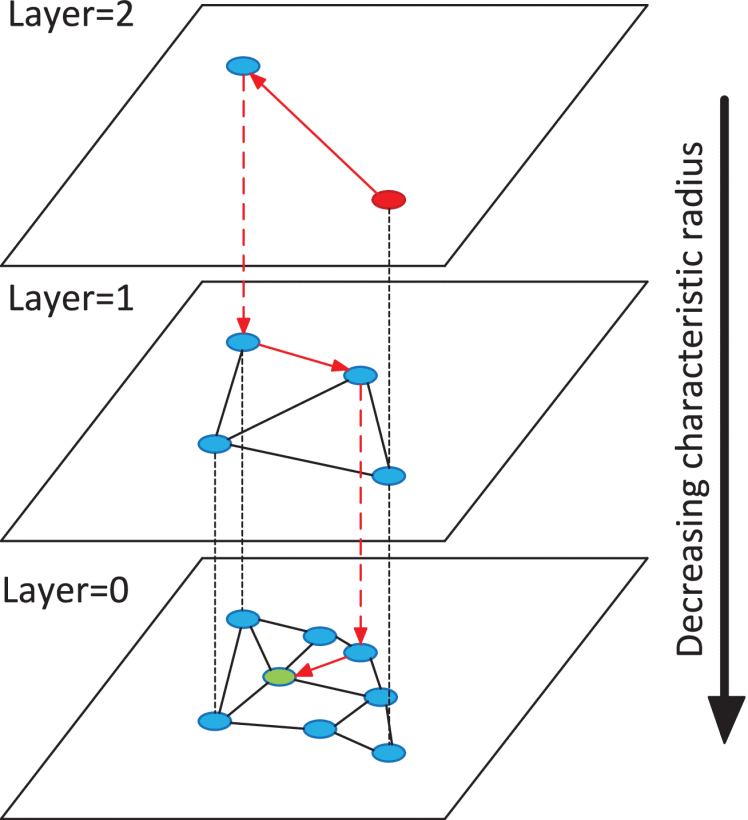
\includegraphics[width=0.3\linewidth]{assets/png/background/hnsw}
    \end{center}

    \caption{Idea behind the HNSW implementation~\cite{malkov_efficient_2020}}
    \label{fig:hnsw}
\end{figure}

\noindent In the context of our thesis, we are not dealing with an exact K-NNS\@.
Exact K-NNS (Section~\ref{subsec:k-nearest-neighbors})~\cite{navarro_searching_2002, tellez_singleton_2016} is feasible when dealing with a small number of data points.
Since it scales linearly with the number of data points, it becomes unfeasible when performing an exact search in a large database.
This is caused by what's known as the \("\)curse of dimensionality\("\). \\ \\
This issue can be overcome by using an approximate K-NNS algorithm~\cite{muja_scalable_2014, houle_rank-based_2015}.
In the case of approximate K-NNS, we \("\)[relax] the condition of the exact search by allowing a small number of errors.\("\)~\cite{malkov_efficient_2020}
Obviously, the search results will not be as exact as those returned by a K-NNS algorithm, but this is acceptable for applications such as an information retrieval system.
Especially in our case, since we also have a filtering system that can help with the retrieval of the most similar documents. \\ \\
This approximate K-NNS and HNSW algorithm has been implemented in Elasticsearch\footnote{https://www.elastic.co/guide/en/elasticsearch/reference/current/knn-search.html\#approximate-knn-limitations}.
The HNSW is used by Elasticsearch to index the dense vectors (document embeddings), while the approximate K-NNS algorithm is used to retrieve the $K$ most similar documents to the query vector.

\subsection{Evaluation Methods}\label{subsec:evaluation-methods}
To measure the performance of an information retrieval system, we can use several different metrics.
These metrics can be divided into two distinct categories: offline metrics~\cite{canamares_offline_2020} and online metrics~\cite{hofmann_online_2016}.
Offline metrics are used to evaluate the performance of the system before this is deployed.
On the other hand, online metrics are used to measure performance after the system has been deployed.
Offline evaluation methods can also be divided into two subgroups, order-unaware and order-aware metrics~\cite{canamares_offline_2020}.
To evaluate our system, we used metrics from both subgroups.

\subsubsection{Order-Unaware Metrics}
In order-unaware metrics, the order of the results does not impact the score of the metric.
The most popular order-unaware metrics are precision (Formula ~\ref{eq:precision-redef}), recall (Formula ~\ref{eq:recall-redef}) and F1 score (Formula ~\ref{eq:f1-redef}).

\begin{equation}
    P@K = \frac{\text{Relevant retrieved documents}}{K}
    \label{eq:precision-redef}
\end{equation}

\begin{equation}
    R@K = \frac{\text{Relevant retrieved documents}}{\text{All relevant documents}}
    \label{eq:recall-redef}
\end{equation}

\begin{equation}
    F1@K = 2 \frac{P@K \cdot R@K}{P@K + R@K}
    \label{eq:f1-redef}
\end{equation}

\noindent All three of these metrics have been used in our evaluation process in the variant $@K$.
Where $K$ is the number of retrieved documents.
This was done to evaluate the system by increasing $K$ and seeing how the metrics evolved the more documents we retrieved.
Moreover, all of these metrics are computed for a single query.
To get the overall precision, recall, and F1 score of the system, we compute the metric $@K$ for each query and divide it by the total number of queries (Formula~\ref{eq:overall}).

\begin{equation}
    \text{$\overline{Metric}$}@K = \frac{1}{Q}\sum_{q=1}^Q \text{Metric}@K_q
    \label{eq:overall}
\end{equation}

\subsubsection{Order-Aware Metrics}
On the other hand, order-aware metrics take into consideration the ordering of the results when computing the score.
The metrics used by us are the average precision (Formula~\ref{eq:ap}) and the mean average precision (Formula~\ref{eq:map})~\cite{yilmaz_new_2008} -- also in this case in their $@K$ variant.

\begin{equation}
    AP@K = \frac{1}{K} \sum_{k=1}^{K} P@k \cdot rel_k
    \label{eq:ap}
\end{equation}

\noindent In the average precision formula, $K$ is the number of relevant results, and $rel_k$ is the binary relevance score for document $k$.
A score of 0 or 1 is given to all the returned documents.
If a 0 is given, this means that the document is not relevant to the query.
On the other hand, 1 means that the document is relevant.

\begin{equation}
    MAP@K = \frac{1}{Q} \sum_{q=1}^{Q} AP@K_q
    \label{eq:map}
\end{equation}
\subsection{t-SNE Plots}\label{subsec:t-sne-plots}
t-SNE is an algorithm used to visualize high-dimensional data in a two- or three-dimensional space~\cite{maaten_visualizing_2008}.
This algorithm is a variation of the Stochastic Neighbor Embedding~\cite{hinton_stochastic_2002}
approach presented in 2002.
The t-SNE variation, according to the authors, is \("\)much easier to
optimize, and it produces significantly better visualizations by reducing the tendency to crowd
points together in the center of the map.\("\)~\cite{maaten_visualizing_2008} \\ \\
In the context of this thesis, the t-SNE plot is used to evaluate the output of the implemented
information retrieval system~\cite{peltonen_information_2015}.
By using t-SNE, we can show the semantic distance between the documents and the queries.


\section{Related Work}\label{sec:related-work}
In this section, we are going to have a look at some of the papers and projects that are in some way related to what we have done with API Scout.
In the first part of this section, we are going to compare our tool with other public OpenAPI aggregators.
Next, we are going to talk about some research that has been done in this field on which we based our work.

\subsection{API Aggregators}\label{subsec:api-aggregators}
As said in Section~\ref{sec:motivation}, there exist many OpenAPI aggregators online.
In Table~\ref{tab:comparison}, we can see a comparison between the main aggregators and API Scout.
As we can see, API Scout contains almost double the amount of API specifications than the sum of specifications contained in all the other aggregators.
Moreover, API Scout has several features that most of the other aggregators don't have.
For example, API Scout stores and returns metadata about the API -- metadata being anything that was not already present in the OpenAPI Specification for that API -- as well as a set of pre-computed metrics.
API Scout offers also the possibility to filter the data using a custom filtering DSL designed by us, as well as offering multiple versions of the same specifications -- i.e.\ a commit history.

\begin{table}[!h]
    \begin{center}
        \begin{tabular}{p{2.2cm} | c c c c c || c}
            \textbf{Feature} & \textbf{APIs.guru} & \textbf{SwaggerHub} & \textbf{Public APIs} & \textbf{Rapid API} & \textbf{API Tracker} & \textbf{API Scout} \\ \hline
            APIs Count & $\sim$2'500 & $\sim$500'00 & $\sim$1'400 & $\sim$40'000 & $\sim$5'600 & $\sim$1'000'000 \\
            Title Searching & \cmark & \cmark & \cmark & \cmark & \cmark & \cmark \\
            Content Searching & \xmark & \cmark & \xmark & \cmark & \xmark & \cmark \\
            Display API Metadata & \xmark & \cmark & \cmark & \cmark & \cmark & \cmark \\
            Display API Metrics & \xmark & \xmark & \xmark & \xmark & \xmark & \cmark \\
            Filtering on API ID & \xmark & \xmark & \xmark & \xmark & \xmark & \cmark \\
            Filtering on Version & \xmark & \cmark & \xmark & \xmark & \xmark & \cmark \\
            Filtering on Metrics & \xmark & \xmark & \xmark & \xmark & \xmark & \cmark \\
            Commit History & \xmark & \cmark & \xmark & \xmark & \xmark & \cmark \\
        \end{tabular}
    \end{center}

    \caption{Comparison between the main OpenAPI Specifications aggregators and API Scout}
    \label{tab:comparison}
\end{table}

\subsection{Research}\label{subsec:research}
In the literature, we can find several different examples of research done in the field of embedding and indexing of OpenAPI Specifications.
These papers represent the groundwork of our thesis.
The research we have found in the literature can be divided into four main categories: API corpus construction, sentence embedding, OpenAPI Specification embedding, and information retrieval systems.

\subsubsection{API Corpus Construction}
In the case of the construction of an API corpus, we have a paper written by Assefi et al.~\cite{assefi_intelligent_2022}, in which they built a custom crawler to retrieve API documentation pages.
In this study, they managed to crawl more than 2.8 million documentation pages.
To retrieve these APIs, they have employed machine learning algorithms to filter out all non-REST APIs while retaining the REST ones.
According to the authors, the objective of this study was to \("\)[allow] researchers and practitioners to harvest a large number of API documentations that can speed up the development of software technologies and reduce the cost of accessing resourceful APIs\("\)~\cite{assefi_intelligent_2022}. \\ \\
Another paper that deals with the construction of an API corpus is Souhaila et al.~\cite{souhaila_serbout_apistic_2024}, where they built a corpus on OpenAPI Specification metrics.
A corpus such as this is extremely useful when trying to study the evolution and structure of an OpenAPI Specification.
In addition to the construction of the corpus, the paper goes more in-depth by also analyzing the collected data.

\subsubsection{Sentence Embedding}
When dealing with the transformation of sentences into vectors, several different methods can be employed.
In particular, the unsupervised algorithms used by Arora et al.~\cite{arora_simple_2019} and Mohammed et al.~\cite{mohammed_state---art_2021} can maintain the semantic meaning of the sentence.
This is particularly useful when creating an information retrieval system which uses semantic similarity as a metric. \\ \\
In addition to these two papers, another one has been published by Mu et al.~\cite{mu_all-but--top_2018}, in which they post-process the embeddings obtained by the embedding algorithms to better capture the semantics of the sentence by removing useless parts of the embedding -- such as the top principal components.

\subsubsection{OpenAPI Specification Embedding}
When dealing in particular with OpenAPI Specifications, some papers have explored using sentence embedding algorithms to create retrieval systems or to cluster similar specifications together -- effectively creating categories of specifications.
In the case of the research done by Kotstein et al.~\cite{kotstein_restberta_2024}, they leveraged the natural language parts of API documentation for the training and fine-tuning of a BERT deep learning model.
The goal of this trained RESTBERT model is to output a set of similar specifications to the one given as input. \\ \\
On the other hand, Lu et al.~\cite{lu_comparing_2024} developed a pipeline to cluster OpenAPI Specifications to create categories.
This pipeline is divided into three main parts -- which have been used as inspiration for our own thesis.
These parts are: preprocessing, vectorization, and clustering.
In the preprocessing step, an OpenAPI Specification is cleaned of all the non-natural language fields, and the keywords are extracted by means of an SBERT model.
The list of extracted keywords is then fed to a GloVe embedding model and a vector embedding for the sentence is generated.
Finally, the Mean Shift algorithm clusters the embeddings to create the API categories.

\subsubsection{Information Retrieval Systems}
Finally, we have a group of papers that deal with information retrieval systems of structured or semi-structured documents.
In the case of both research papers written by Bogner et al.~\cite{bogner_evolvability_2020} and Bragilovski et al.~\cite{bragilovski_how_2024}, they embedded structured data and indexed it in an information retrieval system. \\ \\
On the other hand, Wei et al.~\cite{wei_survey_2023} performed a survey on several existing query-based API information retrieval systems.
From their research, it emerged that in most cases the data regarding the APIs are taken from GitHub.
These systems mostly use either deep learning techniques for the embedding process -- such as BERT -- or other techniques such as Word2Vec.
Finally, for the evaluation of the systems, the most used metrics are precision, recall, accuracy, and mean average precision.

\section{Summary and Outlook}\label{sec:summary-and-outlook}
In this chapter, we have seen what an OpenAPI specification is, and how we can leverage deep-learning models to create vector embeddings representing the semantic meaning of the sentence they are encoding.
Moreover, we have also seen how we can use HNSW to speed up an approximate K-NN search.
Finally, we also had a look at the works in literature that are related with this thesis.
In the following chapters, we will describe the early results, architecture, implementation, deployment, and evaluation of the API Scout tool.


    %%%%%%%%%%%%%%%%%%%%%%%%%%%%%%%%%%%%%%%%%%%%%%%%%%%%%%%%%%%%%%%%%
    %%%	EXPERIMENTATION %%%%%%%%%%%%%%%%%%%%%%%%%%%%%%%%%%%%%%%%%%%%%
    %%%%%%%%%%%%%%%%%%%%%%%%%%%%%%%%%%%%%%%%%%%%%%%%%%%%%%%%%%%%%%%%%

    \chapter{Feasibility Study}\label{ch:experimentation}

With the API Scout platform being a data aggregator for OpenAPI Specifications, we need a way of efficiently indexing and searching through the plethora of crawled documents in our database.
The goal of this experimentation section is to have a better understanding of the technologies and algorithms to use during the development of the platform. \\ \\
In the following sections, we will see an in-depth explanation of how the indexing and retrieval of documents will be implemented, as well as an evaluation of this solution on a test dataset.
The dataset used in this study is composed of \verb|~|3'000 specifications taken from APIs.guru\footnote{https://apis.guru/}.
This dataset has been used in several other research papers on APIs~\cite{ma_restful_2023, kim_empirical_2019, tsai_rest_2021, yasmin_first_2020, moon_api-miner_2022, yang_towards_2018, ma_api_2020}.

\section{Data Analysis}\label{sec:data-analysis}
Before delving further into the approach taken for the indexing and retrieval of the documents, we shall analyze the documents contained in the APIs.guru dataset. \\ \\
During this phase, we had to visualize the semantic relationship of the documents.
To do so, we embedded the documents in 512 dimensions.
Once embedded, we performed a dimensionality reduction using t-SNE\@.
At this point, we added the third dimension representing the category of the document and plotted the points.
The category of the API specification is taken from the \verb|info.x-apisguru-categories| tag manually assigned by APIs.guru. \\ \\
The aforementioned steps produce the result depicted in Figure.
As we can see from both plots, the majority of the documents have been tagged with the \("\)cloud\("\) (\textbf{1}) and \("\)analytics\("\) (\textbf{2}) labels, even though most of them are not tightly clustered together.
Upon closer inspection, though, we can see that most – if not all – documents from the \("\)marketing\("\) (\textbf{3}) category are very close to one another.

\begin{figure}%
    \centering
    \begin{minipage}{.6\textwidth}
        \centering
        \subfloat[\centering API Specifications Color-Coded by \texttt{x-apisguru-categories} field]{{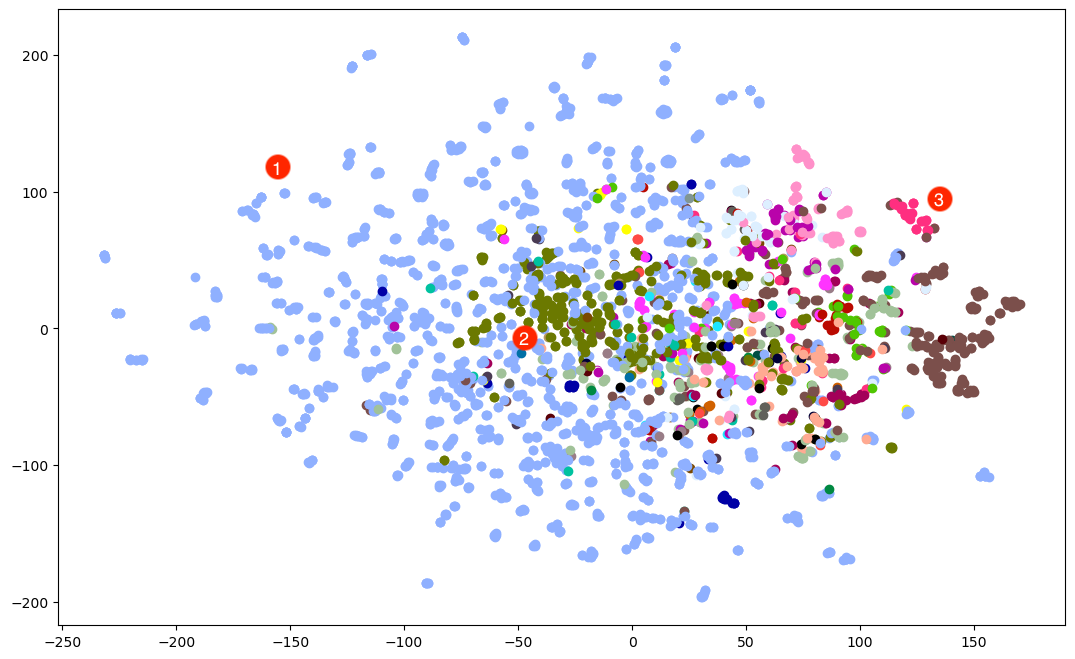
\includegraphics[width=\linewidth]{assets/png/experimentation/categories}}}
    \end{minipage}%
    \begin{minipage}{.4\textwidth}
        \centering
        \subfloat[\centering \texttt{x-apisguru-categories} Word Cloud]{{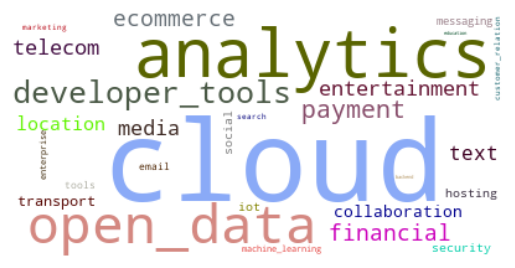
\includegraphics[width=\linewidth]{assets/png/experimentation/cloud}}}
    \end{minipage}

    \caption{Visualization of APIs.guru Dataset by Category and Semantic Relationship}
    \label{fig:documents-plot}
\end{figure}

\section{Approach}\label{sec:approach}
When dealing with OpenAPI Specifications, we are working with JSON or YAML files (which are structured).
Moreover, these files follow the OpenAPI Specifications; thus we know that the documents will contain a very similar structure. \\ \\
Since we are dealing with a very high number of documents, it is paramount to have a fast and reliable index that can be searched through.
For this reason, we decided to use vector embeddings to represent documents in our database.
Embedding models offer a way of transforming documents into vectors of numbers, and -- in our case -- we used Google's Universal Sentence Encoder~\cite{cer_universal_2018} to perform the aforementioned task.
The embedding is done on only a part of the document's content, namely everything that is contained in the~\verb|description|, \verb|name|, \verb|title|, and \verb|summary| tags. \\ \\
We chose to do so because these tags are the only ones that contain natural language descriptions of the API in general or of its endpoints.
After the creation of the embeddings, we saved the vectors -- as well as the name, version, and id -- of the specifications in an Elasticsearch index.
We chose Elasticsearch and the ELK (Elastic-Logstash-Kibana) stack because it is very rapid and scalable.
Moreover, Elasticsearch offers the possibility of searching documents based on the \textit{K}-NN algorithm. \\ \\
This solution seems to be the most promising for the amount of data and hardware availability we have for this project.
We were considering also deep-learning models but discarded them since they are resource intensive and would be overkill for this kind of application.
\section{Ground Truth}\label{sec:ground-truth}
To evaluate the performance of our information retrieval system, we used a ground truth.
Our ground truth consists in a textual file in which we have a query and the expected result.
Some examples are depicted in Figure~\ref{fig:ground-truth}.\\ \\
The file is divided into blocks of two lines.
The first line represents the query that will be vectorized and passed to the $K$-NN query.
On the other hand, the second line represents the title of the document that needs to be found in the top 5 results of the query.
The title of the document on the second line of the block has been chosen manually, this means that we read some of the API specifications and wrote a query that can be connected to that specific document. \\ \\
However, in some cases, there can be multiple documents that satisfy one query; for example, in the case of the query \("\)driving license registration service.\("\)
In the database, there are several different APIs related to the query mentioned: \("\)Transport Department, Tamil Nadu\("\) and \("\)Transport Department, Haryana.\("\)
In such cases, we take the first occurrence that starts with the words \("\)Transport Department.\("\)

\begin{figure}[!h]
    \centering
    \begin{verbatim}
             ...
             aws iot service on secure tunneling
             AWS IoT Secure Tunneling

             driving license registration service
             Transport Department

             sentiment analysis service api
             Text Analytics & Sentiment Analysis API | api.text2data.com

             email mailbox checker
             MailboxValidator Free Email Checker
             ...
    \end{verbatim}
    \caption{Ground Truth}
    \label{fig:ground-truth}
\end{figure}
\section{Evaluation}\label{sec:preliminary-evaluation}

\subsection{Method}\label{subsec:method}
To evaluate the performance of our solution, we used average precision and recall.
In information retrieval systems~\cite{canamares_offline_2020}, precision is defined as the inverse of the position in which the document -- defined in the ground truth -- was found in (Equation~\ref{eq:precision}).
Where $POS$ is the position in which the document was found in ($1$ to $5$ if the document is in the top $5$, $0$ otherwise).
\begin{equation}
    P_i = \frac{1}{POS_i}
    \label{eq:precision}
\end{equation}
The average precision is the average of the precisions among all queries defined in the ground truth (Equation ~\ref{eq:avg-precision}).
Where $N$ is the total number of queries in the ground truth.
\begin{equation}
    \overline{P} = \frac{1}{N} \cdot \sum^N_{i=1}P_i
    \label{eq:avg-precision}
\end{equation}
Finally, the recall is defined as the number of documents found in the top $5$ -- regardless of the position they were found in -- over the total number of queries (Equation~\ref{eq:recall}).
Where $C$ is the number of documents found in the top $5$, and $N$ is the total number of queries in the ground truth.

\begin{equation}
    R = \frac{C}{N}
    \label{eq:recall}
\end{equation}

\subsection{Results}\label{subsec:results}
The results obtained with the embedding + K-NN solution are very promising, as we can see in the t-SNE plot (Figure~\ref{fig:tSNE-plot}, Subsection~\ref{fig:tSNE-plot}). \\ \\
With the \("\)Y\("\) markers representing the queries, and the dots representing the most similar documents found for that query, we can see that the dots and \("\)Y\("\) markers of the same colors are fairly close to each other. \\ \\
Moreover, we performed a validation step with a ground truth.
From the validation step, we concluded that the average precision and recall of the document retrieval are:
\[\overline{P} = 0.6 ~~~~~~ R = 1.0\]
This validation was done on 10 different queries.
The position in which each ground truth appeared in the searches can be found in Figure~\ref{fig:ground-truth-eval}.

\begin{figure}[!h]
    \centering
    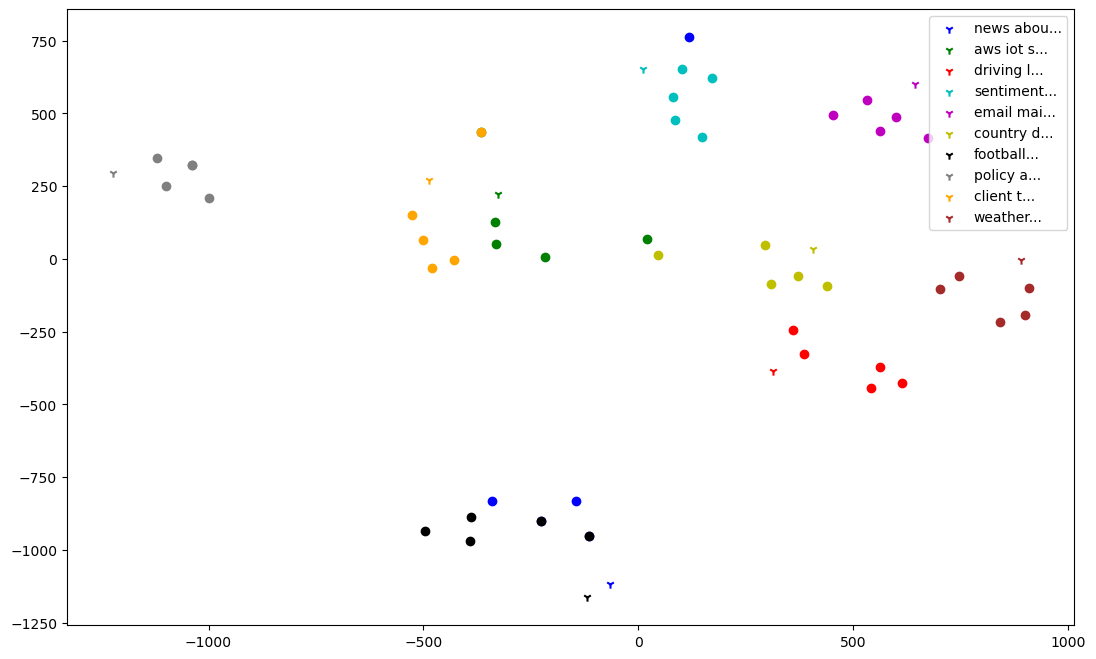
\includegraphics[width=13cm]{assets/png/experimentation/sne}
    \caption{t-SNE Plot}
    \label{fig:tSNE-plot}
\end{figure}

\begin{figure}[!h]
    \begin{verbatim}
  Position in which the ground truth was found:

      "NFL v3 Ply-by-Play" was found at position #1
      "AWS IoT Secure Tunneling" was found at position #4
      "Transport Department" was found at position #4
      "Text Analytics & Sentiment Analysis API | api.text2data.com" was
        found at position #4
      "MailboxValidator Free Email Checker" was found at position #1
      "Interzoid Country Data Standardization API" was found at position #1
      "Soccer v3 Projections" was found at position #1
      "PolicyClient" was found at position #1
      "NetworkManagementClient" was found at position #3
      "Interzoid Get Weather City API" was found at position #2
    \end{verbatim}
    \caption{Ground Truth Evaluation}
    \label{fig:ground-truth-eval}
\end{figure}

\noindent As we can see, all ground truths we found in the top 5 results -- hence $R = 1.0$.
The validation on the ground truth, though, does not paint the full picture of the capabilities this solution offers.
For example, Figure~\ref{fig:query-example} represents the top 5 documents returned by the information retrieval system if we try searching using the query: \("\)american sports news\("\). \\ \\
As we can see in Figure~\ref{fig:query-example}, the engine is able to recognize that both the \textit{NFL} and the \textit{MLB} are professional American sports leagues.
The former being the National Football League, and the latter being the Major League Baseball.
Moreover, it is also able to understand that soccer is a sport and return it. \\ \\
As can be seen both in the average precision ($\overline{P} = 0.6$), and the above example, there are still some noisy results that match part or none of the queries, but this is acceptable.
The reason is that this is not the only means of searching.
To further filter the documents returned by the information retrieval system, we will implement a DSL for the user to specify filters to apply to the output of the natural language query.

\begin{figure}[!h]
    \begin{verbatim}
            These are the top 5 results of the query "american sports news":

                1. NFL v3 Play-by-Play     v.1.0   [67%]
                2. News Plugin             v.1     [66%]
                3. Soccer v3 Projections   v.1.0   [64%]
                4. MLB v3 Projections      v.1.0   [64%]
                5. NFL v3 Scores           v.1.0   [64%]
    \end{verbatim}

    \caption{Example Output of a Query}
    \label{fig:query-example}
\end{figure}
\section{Comparison}\label{sec:comparison}
After validating our system against a tailored ground truth, we compared the results of API Scout with the ones of APIs.guru.
The comparison was performed by taking the queries from the ground truth and searching for them on the APIs.guru website.
The result of this evaluation is depicted in Figure~\ref{fig:apis-guru-eval}.
APIs.guru was not able to yield any document for any of the queries given.
For this reason, APIs.guru's platform has an average precision ($\overline{P}$) of 0 and a recall ($R$) of 0.

\begin{figure}[!h]
    \begin{verbatim}
          Position in which the ground truth was found:

              "NFL v3 Ply-by-Play" was NOT found
              "AWS IoT Secure Tunneling" was NOT found
              "Transport Department" was NOT found
              "Text Analytics & Sentiment Analysis API | api.text2data.com" was
                NOT found
              "MailboxValidator Free Email Checker" was NOT found
              "Interzoid Country Data Standardization API" was NOT found
              "Soccer v3 Projections" was NOT found
              "PolicyClient" was NOT found
              "NetworkManagementClient" was NOT found
              "Interzoid Get Weather City API" was NOT found
    \end{verbatim}
    \caption{APIs.guru Evaluation}
    \label{fig:apis-guru-eval}
\end{figure}



    %%%%%%%%%%%%%%%%%%%%%%%%%%%%%%%%%%%%%%%%%%%%%%%%%%%%%%%%%%%%%%%%%
    %%%	ARCHITECTURE %%%%%%%%%%%%%%%%%%%%%%%%%%%%%%%%%%%%%%%%%%%%%%%%
    %%%%%%%%%%%%%%%%%%%%%%%%%%%%%%%%%%%%%%%%%%%%%%%%%%%%%%%%%%%%%%%%%

    \chapter{Architecture}\label{ch:architecture}
API Scout is divided into three main parts: the backend, the databases, and the model.
A general architecture of the project can be found in Figure~\ref{fig:backend-architecture}.
In the backend, we have all those methods and API endpoints that deal with the embedding, indexing, and retrieval of the OpenAPI specifications.
For storing the data, we use both a MongoDB and an Elasticsearch instance.
The MongoDB instance is used for storing the OpenAPI JSON files.
On the other hand, the Elasticsearch instance is used to store the metadata -- used by the DSL -- and the vector embeddings of the specifications. \\ \\
From a tech stack point of view, we can see in Figure~\ref{fig:languages-architecture} that we used both Elasticsearch and MongoDB for the databases, Tensorflow for the embedding model, and Golang for the backend.

\begin{figure}[h]
    \begin{center}
        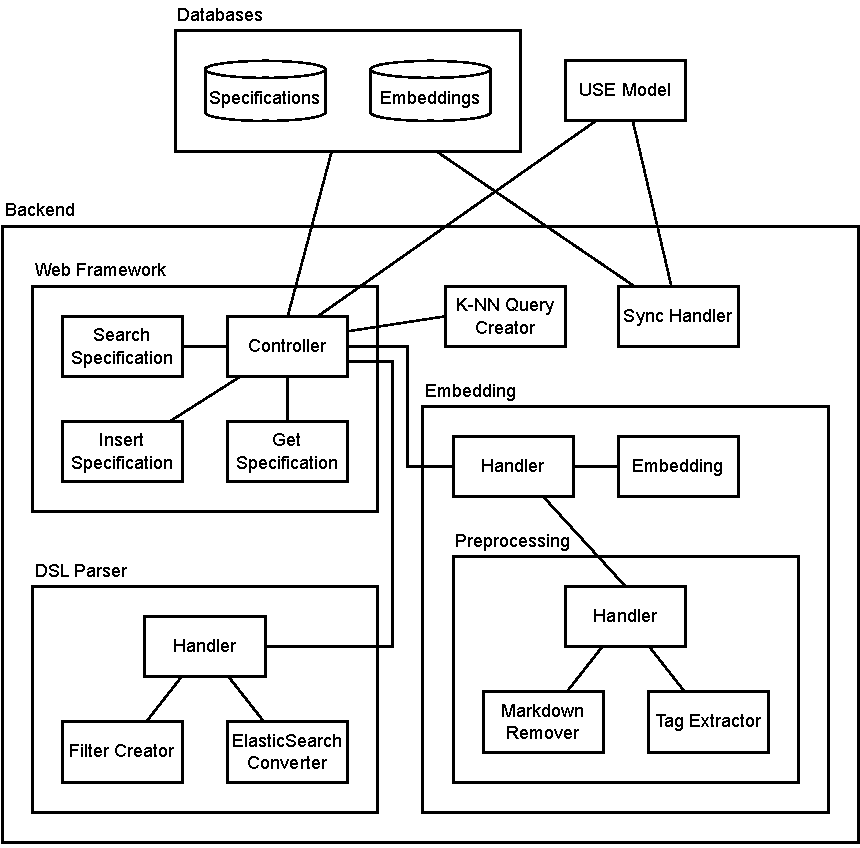
\includegraphics[width=0.6\linewidth]{assets/pdf/architecture/general-architecture}
    \end{center}

    \caption{API Scout's architecture}
    \label{fig:backend-architecture}
\end{figure}

\begin{figure}[h]
    \begin{center}
        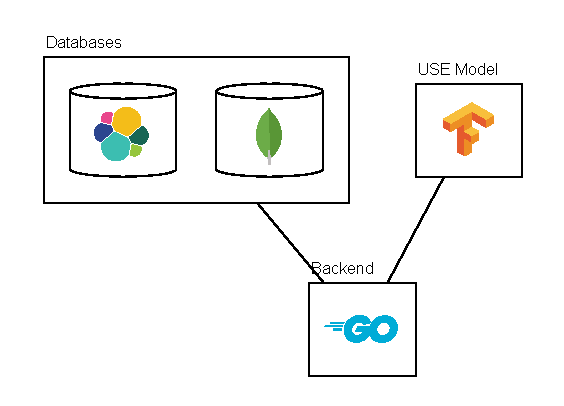
\includegraphics[width=0.6\linewidth]{assets/pdf/architecture/languages-architecture}
    \end{center}

    \caption{API Scout's tech stack}
    \label{fig:languages-architecture}
\end{figure}

\section{Databases}\label{sec:databases}

The system uses two databases to store the data, a MongoDB and an Elasticsearch database.
In the following sections, we will explain more in depth the reasons behind choosing two different databases and how they are used.

\subsection{Specifications Database}\label{subsec:specifications-database}
The specifications database is a MongoDB instance.
Since OpenAPI has multiple versions, and not all API specifications adhere to this standard, it is possible that the specifications have a slightly different structure.
The reason behind choosing only some of the fields of the original dataset is that we consider these to be the most relevant when building a retrieval system and a filtering DSL\@.
We used MongoDB to save the OpenAPI specifications both because MongoDB handles well these kind of JSON/YAML documents, and because other API Analytics services -- outside the scope of this thesis, but which provide the source of the dataset -- rely on such database and data structure~\cite{souhaila_serbout_apistic_2024}. \\ \\
The MongoDB database is composed of two collections, one containing the specifications and one containing the metrics for those specifications.

\subsubsection{Specifications Collection}
In the specifications collection, we have all the specifications that have been scraped from different sources: GitHub, BigQuery, APIs.guru and SwaggerHub~\cite{souhaila_serbout_apistic_2024}.
Moreover, the documents have been saved with two different structures.
The structure of the documents coming from SwaggerHub is described in Listing~\ref{lst:data-swaggerhub} and Table~\ref{tab:data-swaggerhub}.
The structure of the documents coming from GitHub, instead, is described in Listing~\ref{lst:data-github} and Table~\ref{tab:data-github}.
In Tables~\ref{tab:data-swaggerhub} and~\ref{tab:data-github}, we describe what each top-level field in the document means.
In addition, we also highlight those fields that have been used in API Scout.

\begin{lstlisting}[label={lst:data-swaggerhub},language=json,caption={Structure of the data coming from SwaggerHub},captionpos=b]
          {
              "_id": ObjectId("65ce1ae96eb5a9c18ffe38fc"),
              "_fetching_reference": null,
              "_API_reference": "https://api.swaggerhub.com/...",
              "_meta": {},
              "_name": "Bisan Enterprise API",
              "_description": "This is the Bisan...",
              "_created_at": "2020-12-15T09:42:49Z",
              "_last_modified": "2020-12-15T09:42:49Z",
              "_created_by": "mbanna",
              "_API_url": "https://api.swaggerhub.com/.../1.0.1",
              "_version": "1.0.1",
              "_OPENAPI_version": "3.0.0",
              "_API_spec_hash": null,
              "_API_url_hash": "7b88c0cjh4a34vdb78...",
              "api": {}
          }
\end{lstlisting}

\begin{lstlisting}[label={lst:data-github},language=json,caption={Structure of the data coming from GitHub},captionpos=b]
           {
               "_id": ObjectId("65ce1ae96eb5a9c18ffe38fc"),
               "id": 187463,
               "api_spec_id": 472773,
               "api_title": "math-api-v1",
               "api_version": "1.0",
               "commit_date": 2019-11-27T12:31:23.000+00:00,
               "commits": 1,
               "processed_at": 2023-11-27T12:31:23.000+00:00,
               "sha": "vsd876vs68df68fs...",
               "url": "https://raw.githubusercontent.com/...",
               "latest": true,
               "api": {}
           }
\end{lstlisting}

\subsubsection{Metrics Collection}
In the metrics collection, we have one document for each specification.
The connection between the documents is done through the MongoID. If the MongoID in the specification collection and the one in the metrics collection are the same, this means that the two documents are related.
The metrics documents store some statistics about the corresponding OpenAPI specification.
Listing~\ref{lst:data-metrics} and Table~\ref{tab:data-metrics} describe the structure of these documents.
Moreover, as before, we also highlight those fields that have been used in API Scout.

\begin{lstlisting}[label={lst:data-metrics},language=json,caption={Structure of the specification's metrics data},captionpos=b]
            {
                "_id": ObjectId("65ce1ae96eb5a9c18ffe38fc"),
                "securityData": {
                    "schemes": [],
                    "endpointsCount": 20,
                    "average": 10
                },
                "schemas": [],
                "schemaSize": {
                    "schemas": 3,
                    "defined_schemas": 3,
                    "properties": 5,
                    "max_properties": 2,
                    "min_properties": 1
                },
                "structureSize": {
                    "paths": 3,
                    "operations": 3,
                    "used_methods": 3,
                    "used_parameters": 2
                },
                "documentationsData": {}
            }
\end{lstlisting}

\begin{table}[!h]
    \begin{center}
        \begin{tabular}{l p{11cm} c}
            \hline
            \textbf{Field} & \textbf{Description} & \textbf{Used} \\ \hline
            \verb|_id| & The ID given to the document by MongoDB & \cmark \\
            \verb|_fetching_reference| & The ID given by the crawler to the document & \xmark \\
            \verb|_API_reference| & The URL of the API & \xmark \\
            \verb|_meta| & Some metadata on the API server and validity of the JSON specification & \xmark \\
            \verb|_name| & The name of the API (taken from the API specification) & \cmark \\
            \verb|_description| & The description of the API (taken from the API specification) & \xmark \\
            \verb|_created_at| & The date of creation of the API & \cmark \\
            \verb|_last_modified| & The date the API was last modified & \xmark \\
            \verb|_created_by| & The user that uploaded the API specification & \xmark \\
            \verb|_API_url| & The specific URL for the specification version & \xmark \\
            \verb|_version| & The API version & \cmark \\
            \verb|_OPENAPI_version| & The OpenAPI version used in the specification & \cmark \\
            \verb|_API_spec_hash| & The specification hash & \xmark \\
            \verb|_API_url_hash| & The URL hash & \xmark \\
            \verb|api| & The object containing the API specification & \cmark \\ \hline
        \end{tabular}
    \end{center}

    \caption{Description of the data contained in a SwaggerHub document}
    \label{tab:data-swaggerhub}
\end{table}

\begin{table}[!h]
    \begin{center}
        \begin{tabular}{l l c}
            \hline
            \textbf{Field} & \textbf{Description} & \textbf{Used} \\ \hline
            \verb|_id| & The ID given to the document by MongoDB & \cmark \\
            \verb|id| & The ID of the API specification's commit & \xmark \\
            \verb|api_spec_id| & The ID of the API specification & \cmark \\
            \verb|api_title| & The name of the API & \cmark \\
            \verb|api_version| & The version of the API & \cmark \\
            \verb|commit_date| & The time at which this version was committed & \cmark \\
            \verb|commits| & The number of commits this API has in total & \cmark \\
            \verb|processed_at| & The time at which the API was processed by the crawler & \xmark \\
            \verb|sha| & The hash of the specification & \xmark \\
            \verb|url| & The URL of the specification & \xmark \\
            \verb|latest| & If the current commit is the latest or not & \cmark \\
            \verb|api| & The object containing the API specification & \cmark \\ \hline
        \end{tabular}
    \end{center}

    \caption{Description of the data contained in a GitHub document}
    \label{tab:data-github}
\end{table}

\begin{table}[!h]
    \begin{center}
        \begin{tabular}{l p{9.5cm} c}
            \hline
            \textbf{Field} & \textbf{Description} & \textbf{Used} \\ \hline
            \verb|_id| & The ID given to the document by MongoDB & \cmark \\
            \verb|securityData.schemes| & A list of all the security schemes present in the specification & \xmark \\
            \verb|securityData.endpointsCount| & The number of endpoints covered by some kind of security schema & \cmark \\
            \verb|securityData.average| & The average number of endpoints covered by some kind of security schema & \xmark \\
            \verb|schemas| & A list of all the schemas present in the specification & \xmark \\
            \verb|schemaSize.schemas| & The number of schemas used in the specification & \cmark \\
            \verb|schemaSize.defined_schemas| & The number of defined schemas in the specification & \xmark \\
            \verb|schemaSize.properties| & The number of properties used in the specification & \cmark \\
            \verb|schemaSize.max_properties| & The maximum number of properties used in a schema & \xmark \\
            \verb|schemaSize.min_properties| & The minimum number of properties used in a schema & \xmark \\
            \verb|structureSize.paths| & The number of paths in the specification & \cmark \\
            \verb|structureSize.operations| & The number of operations in the specification & \cmark \\
            \verb|structureSize.used_methods| & The number of methods used in the specification & \cmark \\
            \verb|structureSize.used_parameters| & The number of parameters used in the specification & \xmark \\
            \verb|documentationsData| & Object containing metrics about the documentation of endpoints & \xmark \\ \hline
        \end{tabular}
    \end{center}

    \caption{Description of the data contained in a metrics document}
    \label{tab:data-metrics}
\end{table}

\subsection{Embeddings Database}\label{subsec:embeddings-database}
To search for API specifications by querying their natural language descriptions, however, we need to save the vectorization of the natural language extracted from the OpenAPI Specification somewhere.
Since the MongoDB data structure could not be modified, the chosen database for storing the vectors was Elasticsearch -- which also contains metadata and metrics of the API specifications. \\ \\
The reason behind choosing Elasticsearch is that it offers out-of-the-box solutions to deal with textual embeddings.
For instance, the embeddings -- when indexed -- are saved into a Hierarchical Navigable Small World graph (Section ~\ref{subsec:hierarchical-navigable-small-world-graphs}), which helps with retrieval performance.
In addition, it already offers an approximate K-NN search (Section~\ref{subsec:hierarchical-navigable-small-world-graphs}) API with the possibility of pre- or post-filtering the data.
The aforementioned metadata and metrics are used to pre-filter the data in the K-NN search queries.

\section{Universal Sentence Encoder Model}\label{sec:use-model}

To create the vector embeddings of the OpenAPI specifications, we rely on an external Docker container.
This Docker container is based on the \verb|tensorflow/serving| image, which enables us to perform REST API calls to the deep learning model we use for the embedding.
The model chosen for this project is the Universal Sentence Encoder (USE) by Google (Section~\ref{subsec:document-embedding}). \\ \\
The model, after being sent some text fragments as input, will return one 512-dimension vector embedding for each fragment sent to the model.
In practice, the Docker compose requires the request to be structured as in Listing~\ref{lst:model-request}, and the response to be structured as in Listing~\ref{lst:model-response}.

\begin{center}
    \begin{lstlisting}[label={lst:model-request},language=json,caption={Example of request body sent to the model},captionpos=b]
                       {
                           "instances": [
                               "a random fragment",
                               ...
                           ]
                       }
    \end{lstlisting}
\end{center}

\begin{center}
    \begin{lstlisting}[label={lst:model-response},language=json,caption={Example of response body sent to the model},captionpos=b]
                           {
                               "predictions": [
                                   [
                                       0.12321,
                                       0.23123,
                                       ...
                                   ],
                                   ...
                               ]
                           }
    \end{lstlisting}
\end{center}

\section{Web Framework}\label{sec:web-framework-1}
The Web framework module handles all the connections made by external users to the service.
The framework publishes several different endpoints, as well as a Swagger documentation page of the exposed endpoints. \\ \\
The endpoints handle the basic operations of the tool, namely indexing, searching, and retrieving.
Moreover, there are two more endpoints that are used as helpers for migration of the data and evaluation of the system's performance.

\subsection{Indexing Endpoint}\label{subsec:indexing-endpoint-1}
The indexing endpoint (\verb|POST| \verb|/api/v1/specification|) is used to insert new OpenAPI specifications in both MongoDB and Elasticsearch (Figure~\ref{fig:flow-index}). \\ \\
The endpoint takes an OpenAPI specification wrapped in an \verb|api| object, it extracts the natural language fields from it, and then passes it to the main pipeline.
The pipeline is composed of an embedding pipeline component -- which creates the vector embeddings for the specification, and an indexing component.
The latter is used to structure the specification in the correct way and send it both to MongoDB and to Elasticsearch.
To MongoDB, it will send the entire specification, while to Elasticsearch it will send the metadata -- if present -- together with the vector embedding of the document.

\begin{figure}[!h]
    \begin{center}
        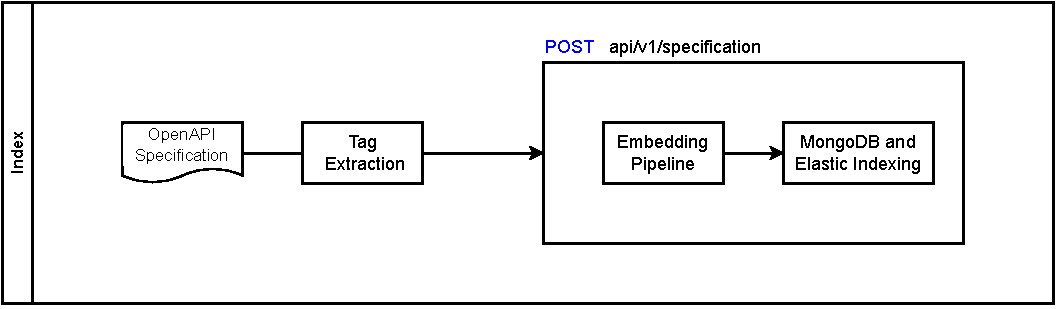
\includegraphics[width=0.8\linewidth]{assets/pdf/architecture/flow-index}
    \end{center}

    \caption{Conceptual view of the indexing pipeline}
    \label{fig:flow-index}
\end{figure}

\subsection{Search Endpoint}\label{subsec:search-endpoint-1}
In the case of the search endpoint (\verb|POST| \verb|/api/v1/search|), the user will be able to send either a specification fragment or a query, some filters, and parameters relative to the pagination and the K-NN query (Figure~\ref{fig:flow-search}).
The reason we chose a \verb|POST| request instead of a \verb|GET| request, is that the query plus the filters would have resulted in a URL that could be too long for the browser or tool to handle, thus we opted for a \verb|POST| request with a body. \\ \\
After passing a query or a specification to the endpoint, it will be preprocessed and fed to the main pipeline.
This pipeline consists of two main components, the embedding pipeline component and the DSL parsing component.
While the former creates the vector embedding from the preprocessed specification, the latter will extract the DSL field of the request and translate our DSL language into API calls that Elasticsearch uses to make its API calls.
Finally, the search query is sent to Elasticsearch, which will retrieve the most similar documents to the query.
Moreover, several calls will be made to MongoDB to retrieve the json specifications -- if requested by the user.

\begin{figure}[!h]
    \begin{center}
        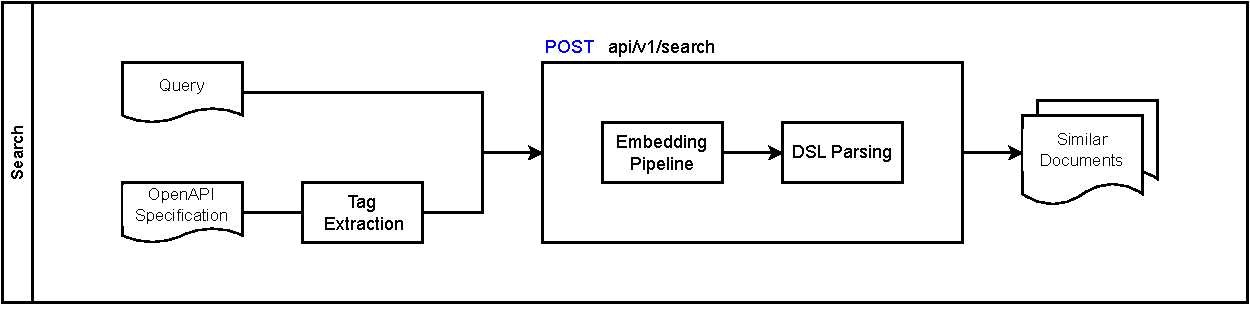
\includegraphics[width=0.9\linewidth]{assets/pdf/architecture/flow-search}
    \end{center}

    \caption{Conceptual view of the search pipeline}
    \label{fig:flow-search}
\end{figure}

\subsection{Retrieval Endpoint}\label{subsec:retrieval-endpoint-1}
The retrieval endpoint (\verb|GET| \verb|/api/v1/specification/{id}|) is used to get a specific OpenApi specification (Figure~\ref{fig:flow-retrieve}).
This endpoint will simply search for the given id in both the Elasticsearch and MongoDB databases, and return a document which will be a combination of the two documents returned by the two databases.

\begin{figure}[!h]
    \begin{center}
        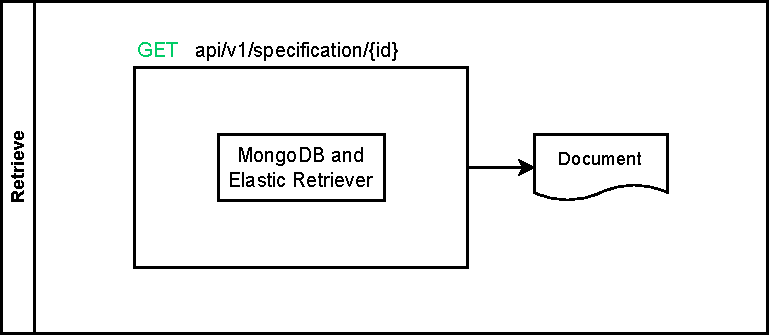
\includegraphics[width=0.5\linewidth]{assets/pdf/architecture/flow-retrieve}
    \end{center}

    \caption{Conceptual view of the retrieval pipeline}
    \label{fig:flow-retrieve}
\end{figure}

\subsection{Preprocessing Endpoint}\label{subsec:preprocessing-endpoint-1}
The preprocessing endpoint (\verb|POST| \verb|/api/v1/preprocess|) is used to simulate the preprocessing step for a search query (Figure~\ref{fig:flow-preprocess}).
This endpoint has been implemented has a helper endpoint during the evaluation process of this thesis. \\ \\
A document or query is passed as input to the endpoint.
The document will then go through a preprocessing pipeline.
In this pipeline, all the natural language tags will be extracted from the document, and then the resulting string will be cleaned of every markdown structure.
The endpoint will then return to the user a string representing the cleaned version of the input.
In a normal scenario -- i.e.\ in the case of a search or indexing query -- this string will be passed to the embedding model which will use the text to create a vector embedding for the OpenAPI specification or the query.

\begin{figure}[!h]
    \begin{center}
        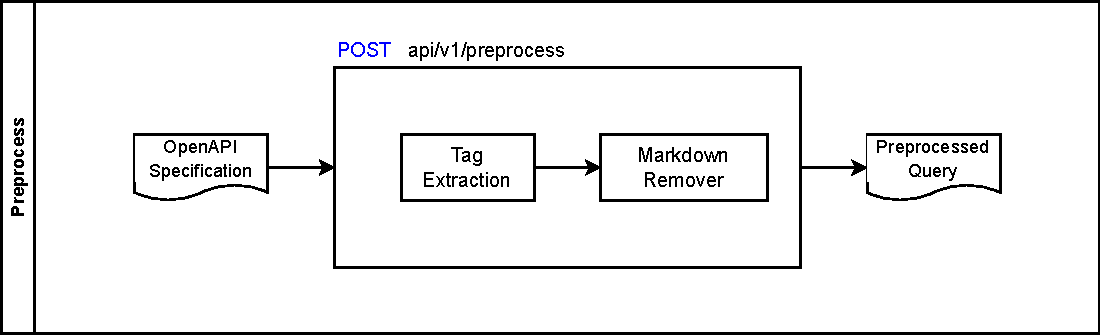
\includegraphics[width=0.8\linewidth]{assets/pdf/architecture/flow-preprocess}
    \end{center}

    \caption{Conceptual view of the preprocessing pipeline}
    \label{fig:flow-preprocess}
\end{figure}

\subsection{Synchronization Endpoint}\label{subsec:synchronization-endpoint-1}
The synchronization endpoint (\verb|PUT| \verb|/api/v1/sync|) is an idempotent endpoint used to index documents that are present in the MongoDB database in Elasticsearch (Figure~\ref{fig:flow-sync}). \\ \\
This endpoint will make sure that the two databases are always in sync.
If, while going through the MongoDB documents, it finds a document that is already in the Elasticsearch database, then it will not insert it again -- from here the idempotence and the choosing of the \verb|PUT| method for this endpoint.

\begin{figure}[!h]
    \begin{center}
        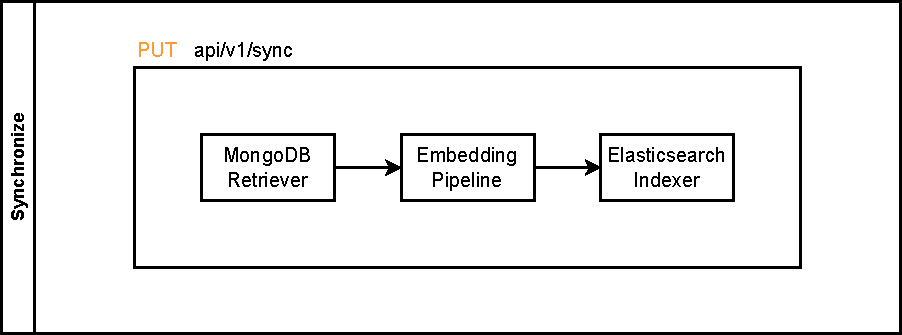
\includegraphics[width=0.7\linewidth]{assets/pdf/architecture/flow-sync}
    \end{center}

    \caption{Conceptual view of the synchronization pipeline}
    \label{fig:flow-sync}
\end{figure}

\section{Preprocessing and Embedding}\label{sec:preprocessing-and-embedding}
Preprocessing and embedding of queries are done inside the \verb|embedding| group of components.
In this group, the system receives the embedding from the web framework controller, and starts the embedding process.
Before transforming the specification into a vector of floating point numbers, it must be preprocessed. \\ \\
In the preprocessing stage, we extract all the specification tags that contain natural language.
After the extraction of these values, they are all inserted into a string which is passed to the Markdown remover component.
This component will strip from the string all of those symbols and structures that are used to defined Markdown components.
Moreover, the string is cleaned of all URL, even if they are not in a Markdown format. \\ \\
Once the string has been properly cleaned, it is passed to the USE model via a POST request.
The model will then return a 512-dimension array of floating point numbers representing the string in a 512-dimensional space.



    %%%%%%%%%%%%%%%%%%%%%%%%%%%%%%%%%%%%%%%%%%%%%%%%%%%%%%%%%%%%%%%%%
    %%%	FILTERING DSL %%%%%%%%%%%%%%%%%%%%%%%%%%%%%%%%%%%%%%%%%%%%%%%
    %%%%%%%%%%%%%%%%%%%%%%%%%%%%%%%%%%%%%%%%%%%%%%%%%%%%%%%%%%%%%%%%%

    \chapter{Filtering DSL}\label{ch:filtering-dsl}
The filtering DSL compiler is a collection of components that handle the logic for the translation of our DSL into a query that can be understood by the Elasticsearch search API\@.
Let's begin the description of the compiler by understanding the reason behind why we decided to implement it.
API Scout is a tool that is mainly aimed at researchers to perform any kind of empirical study on a subset of our APIs. \\ \\
Let's take a real-world scenario.
Let's say that some researchers are conducting a study on the evolution of security in REST API endpoints over time.
First of all, they want to find some APIs that have more than a couple of commits in their history, as well as a number of paths between 10 and 100.
To do so, they could use the filters in Figure~\ref{fig:filter-commits} to retrieve all APIs with more than two commits in their history, and with a number of paths between 10 and 100.

\begin{figure}[!h]
    \begin{center}
        \verb|api.commits>2 metrics.structure.paths<>(10,100]|
    \end{center}

    \caption{Filter on the number of commits and paths of an API}
    \label{fig:filter-commits}
\end{figure}

\noindent As you can see, the structure of the filter is pretty straight-forward, we have the name of the field to filter for on the left-hand side (\verb|api.commits|), the operator in the middle (\verb|>|), and the value on the right-hand side (\verb|2|).
In the case of the range operator (\verb|<>|), the right-hand side is a little bit more complex.
The round parenthesis indicates that 10 must not be included in the range (thus \verb|>10|), while the square bracket indicates that 100 must be included in the range (thus \verb|<=100|).
Moreover, the space between the filters indicates a logic AND operation.
Thus, the resulting APIs must have more than 2 commits, AND a number of paths between 10 (not included), and 100 (included). \\ \\
The researchers will now have IDs of several APIs with more than two commits in their history.
What they would like to do now is to retrieve the commit history for those APIs.
To do so, they can do one search request for each API ID in which they use the filter in Figure~\ref{fig:filter-apis}.
This filter tells API Scout to only retrieve those specifications that have that specific API ID -- i.e.\ the commit history for that API\@.

\begin{figure}[!h]
    \begin{center}
        \verb|api.id==306512|
    \end{center}

    \caption{Filter on a specific API ID}
    \label{fig:filter-apis}
\end{figure}

\noindent Finally, the researchers will now be able to analyze how the security of the endpoints evolved in time, since API scout will return them metadata about the specifications, as well as the full JSON specification.
In the following sections, we will describe the inner workings of the language, including the grammar and its components.

\section{Grammar}\label{sec:grammar}
In Figure~\ref{fig:bnf}, we have the BNF (Backus Normal Form) notation of our filtering DSL\@.
It is important to note that part of this grammar -- namely the \textlangle~version \textrangle~and \textlangle~version core \textrangle~non-terminals -- as well as the MAJOR, MINOR, PATCH, PRERELEASE, and BUILD tokens -- are taken from the official semantic versioning page \footnote{https://github.com/semver/semver/blob/master/semver.md}.
As we can see, several tokens are also used to represent terminals in our grammar.
The tokens are SPACE, PARAMETER, STRING, DATE, BOOLEAN, INTEGER, MAJOR, MINOR, PATCH, PRERELEASE, and BUILD\@.
All of these tokens will be discussed more in detail in the following sections of this chapter. \\ \\
In particular, PARAMETER is discussed in Section~\ref{sec:parameters}.
STRING, DATE, BOOLEAN, and INTEGER are discussed in Section~\ref{sec:types}.
MAJOR, MINOR, PATCH, PRERELEASE, and BUILD are discussed in Section~\ref{sec:types}.

\begin{figure}[!h]
    \begin{center}
        \begin{bnf}
            \textlangle~group \textrangle ::= \textlangle~filter \textrangle | \textlangle~filter \textrangle~SPACE \textlangle~group \textrangle
            ;;
            \textlangle~filter \textrangle ::= \textlangle~lhs \textrangle \textlangle~operator \textrangle \textlangle~rhs \textrangle
            ;;
            \textlangle~lhs \textrangle ::= PARAMETER
            ;;
            \textlangle~rhs \textrangle ::= STRING | DATE | BOOLEAN | INTEGER | \textlangle~version \textrangle | \textlangle~range \textrangle
            ;;
            \textlangle~operator \textrangle ::= '==' | '!=' | '\textasciitilde=' | '<>' | '>=' | '<=' | '>' | '<'
            ;;
            \textlangle~range \textrangle ::= \textlangle~bracket \textrangle \textlangle~limit \textrangle~',' \textlangle~limit \textrangle \textlangle~bracket \textrangle
            ;;
            \textlangle~bracket \textrangle ::= '[' | '(' | ']' | ')'
            ;;
            \textlangle~limit \textrangle ::= INTEGER | DATE | \textlangle~version \textrangle
            ;;
            \textlangle~version \textrangle ::= \textlangle~version core \textrangle | \textlangle~version core \textrangle~'-' PRERELEASE | \textlangle~version core \textrangle~'+' BUILD | \textlangle~version core \textrangle~'-' PRERELEASE '+' BUILD
            ;;
            \textlangle~version core \textrangle ::= MAJOR '.' MINOR '.' PATCH
        \end{bnf}
    \end{center}

    \caption{Filtering DSL in the BNF notation}
    \label{fig:bnf}
\end{figure}

\section{Structure}\label{sec:structure}
As we saw in Section~\ref{sec:grammar}, filters are composed of three main parts: a left-hand side -- the parameter, an operator, and a right-hand side -- the value.
To concatenate multiple filters, just separate them with a space.
The space between the filters is interpreted as an AND operator.
The filters described in Listing~\ref{fig:example-filters} are some examples of valid filters.
For example, let's take \verb|api.version.raw<>(1.0.0,2.0.0]|.
In this case, \verb|api.version.raw| is the parameter, \verb|<>| is the range operator, and \verb|(1.0.0,2.0.0]| is the value, in this case the range. \\ \\
In order for the filter to be valid, it must meet several requirements.
These requirements are:

\begin{enumerate}
    \item The parameter must be valid -- i.e.\ it should exist;
    \item The map of supported types of the operator must contain the type of the parameter;
    \item The value's type must match the parameter's type;
    \item In the case of the range operator's right-hand side:
    \begin{itemize}
        \item The range must be surrounded by either square or round brackets, opened to the left of the range and closed to the right of the range;
        \item The range must be composed of only two elements;
        \item The types of the range delimiters must match the ones of the parameter.
    \end{itemize}
\end{enumerate}

\begin{figure}[!h]
    \begin{center}
        \verb|api.version.raw<>(1.0.0,2.0.0]| \\
        \verb|api.name~="weather"| \\
        \verb|api.commits>=10|
    \end{center}

    \caption{Examples of valid filters}
    \label{fig:example-filters}
\end{figure}

\section{Types}\label{sec:types}
The types supported by our service are explained in Table~\ref{tab:types}.
These types are then used to check that the filters are valid.
The types supported by the API Scout DSL range from the most classic types, such as \("\)string\("\), \("\)integer\("\), and \("\)boolean\("\), to more specific ones such as \("\)version\("\), \("\)date\("\), and \("\)range\("\).
Where \("\)version\("\) is taken from the semver website \footnote{https://semver.org/}, and \("\)range\("\) is a custom type made for this DSL\@.

\begin{table}[!h]
    \begin{center}
        \begin{tabular}{l p{15cm}}
            \hline
            \textbf{Name} & \textbf{Description} \\ \hline
            \verb|string| & An alphanumeric set of characters, must be contained inside \verb|""|, and can contain spaces \\
            \verb|integer| & A positive integer number \\
            \verb|boolean| & A \verb|true| or \verb|false| value \\
            \verb|version| & A semantically valid version (must follow the semantic versioning standard~\cite{preston-werner_semantic_nodate}) (e.g.\ 1.0.0-alpha+c3bh3h) \\
            \verb|date| & A date formatted as \verb|dd/mm/yyyy| (e.g.\ 31/12/2021) \\
            \verb|range| & A set of ordered values contained between two limits.
            The limits can be of integer, version, or date type (e.g. \verb|[12,24)|, \verb|[1.0.0,3.0.0]|, or \verb|(15/05/2022,16/07/2023)|) \\ \hline
        \end{tabular}
    \end{center}

    \caption{List of all the supported types}
    \label{tab:types}
\end{table}
\section{Parameters}\label{sec:parameters}
To filter the result, several different categories of parameters are available.
The filter parameters are divided in API, specification, and metrics categories. \\ \\
In the case of the API category, we have all those parameters that are connected to the extracted metadata about the API (not the specification).
In Table~\ref{tab:parameters-api}, we describe all the parameters in this category with their type and a short description.
Table~\ref{tab:parameters-specification} describes the parameters in the specification category.
These are the parameters relative to the metadata extracted from the OpenAPI specification.
Finally, Table~\ref{tab:parameters-metrics} describes the parameters in the metrics category.
These parameters are connected with the metric values of the specifications~\cite{souhaila_serbout_apistic_2024}.

\begin{table}[H]
    \begin{center}
        \begin{tabular}{l l p{9cm}}
            \hline
            \textbf{Name} & \textbf{Type} & \textbf{Description} \\ \hline
            \verb|date| & date & The date when the API was published \\
            \verb|length| & integer, range & The length of the natural language content string of the API  \\
            \verb|api.name| & string & The name of the API \\
            \verb|api.commits| & integer, range & The number of commits found for that API \\
            \verb|api.latest| & boolean & If the given version of the API is the latest \\
            \verb|api.source| & string & The source where the API was extracted from \\
            \verb|api.version.raw| & version, range & The complete version of the api, e.g.\ 1.0.0-alpha.1 \\
            \verb|api.version.valid| & boolean & If the version is compliant with the semantic versioning standard~\cite{preston-werner_semantic_nodate} \\
            \verb|api.version.major| & integer, range & The part of the version containing the major version number \\
            \verb|api.version.minor| & integer, range & The part of the version containing the minor version number \\
            \verb|api.version.patch| & integer, range & The part of the version containing the patch version number \\
            \verb|api.version.prerelease| & string & The part of the version containing the prerelease string \\
            \verb|api.version.build| & string & The part of the version containing the build string \\ \hline
        \end{tabular}
    \end{center}

    \caption{API parameters descriptions}
    \label{tab:parameters-api}
\end{table}

\begin{table}[!h]
    \begin{center}
        \begin{tabular}{l l p{7cm}}
            \hline
            \textbf{Name} & \textbf{Type} & \textbf{Description} \\ \hline
            \verb|specification.type| & string & The type of openAPI specification, can be \verb|specification.openapi| or \verb|swagger| \\
            \verb|specification.version.raw| & version, range & The complete version of the api, e.g.\ 1.0.0-alpha.1 \\
            \verb|specification.version.valid| & boolean & If the version is compliant with the semantic versioning standard~\cite{preston-werner_semantic_nodate} \\
            \verb|specification.version.major| & integer, range & The part of the version containing the major version number \\
            \verb|specification.version.minor| & integer, range & The part of the version containing the minor version number \\
            \verb|specification.version.patch| & integer, range & The part of the version containing the patch version number \\
            \verb|specification.version.prerelease| & string & The part of the version containing the prerelease string \\
            \verb|specification.version.build| & string & The part of the version containing the build string \\ \hline
        \end{tabular}
    \end{center}

    \caption{Specification parameters descriptions}
    \label{tab:parameters-specification}
\end{table}

\begin{table}[!h]
    \begin{center}
        \begin{tabular}{l c p{8cm}}
            \hline
            \textbf{Name} & \textbf{Type} & \textbf{Description} \\ \hline
            \verb|metrics.security.endpoints| & integer, range & The number of API endpoints which explicitly employ specific security schemes~\cite{souhaila_serbout_apistic_2024} \\
            \verb|metrics.schema.models| & integer, range & The number of data models present in the specification \\
            \verb|metrics.schema.properties| & integer, range & The number of properties within the data models in the specification \\
            \verb|metrics.structure.paths| & integer, range & The number of paths in the specification \\
            \verb|metrics.structure.operations| & integer, range & The number of operations in the specification \\
            \verb|metrics.structure.methods| & integer, range & The number of operations in the specification that use HTTP methods (GET, POST, PUT\ldots) \\ \hline
        \end{tabular}
    \end{center}

    \caption{Metrics parameters descriptions}
    \label{tab:parameters-metrics}
\end{table}

\section{Operators}\label{sec:operators}
To complete the DSL structure, we have defined several different operators.
These operators can be used to compare values of specific types with each other.
The operators supported by API Scout are described in Table~\ref{tab:operators}. \\ \\
In the case of the range operation, the parser will decompose the filter into two different filters.
For example, let's take the range \verb|[23,12)|.
Based on the type of parentheses, the parser will create two different filters.
In this case, it will create both a \verb|>=23| and a \verb|<12| filter.
The full list of parentheses conversions is shown in Table~\ref{tab:conversion-table}.

\begin{table}[!h]
    \begin{center}
        \begin{tabular}{c c p{2.5cm} p{9cm}}
            \hline
            \textbf{Operator} & \textbf{Name} & \textbf{Supported Types} & \textbf{Description} \\ \hline
            \verb|==| & Equal & boolean, string, integer, version, date & Check if two values are the same \\
            \verb|!=| & Not Equal & boolean, string, integer, version, date & Check if two values are different \\
            \verb|~=| & Contain & string, version & Check if the right-hand side of the filter is contained in the parameter's value \\
            \verb|<>| & Range & integer, version, date & Check if the right-hand side of the filter is contained in the given range \\
            \verb|>| & Greater & integer, version, date & Check if the right-hand side value is strictly greater than the left-hand side value \\
            \verb|<| & Less & integer, version, date & Check if the right-hand side value is strictly less than the left-hand side value \\
            \verb|>=| & Greater Equal & integer, version, date & Check if the right-hand side value is greater or equal to the left-hand side value \\
            \verb|<=| & Less Equal & integer, version, date & Check if the right-hand side value is less than or equal to the left-hand side value \\ \hline
        \end{tabular}
    \end{center}

    \caption{Operators descriptions}
    \label{tab:operators}
\end{table}

\begin{table}[!h]
    \begin{center}
        \begin{tabular}{c c}
            \hline
            \textbf{Parenthesis} & \textbf{Operator} \\ \hline
            \verb|[| & \verb|>=| \\
            \verb|]| & \verb|<=| \\
            \verb|(| & \verb|>| \\
            \verb|)| & \verb|<| \\ \hline
        \end{tabular}
    \end{center}

    \caption{Parentheses conversion table}
    \label{tab:conversion-table}
\end{table}



    %%%%%%%%%%%%%%%%%%%%%%%%%%%%%%%%%%%%%%%%%%%%%%%%%%%%%%%%%%%%%%%%%
    %%%	IMPLEMENTATION %%%%%%%%%%%%%%%%%%%%%%%%%%%%%%%%%%%%%%%%%%%%%%
    %%%%%%%%%%%%%%%%%%%%%%%%%%%%%%%%%%%%%%%%%%%%%%%%%%%%%%%%%%%%%%%%%

    \chapter{Implementation}\label{ch:implementation}

\section{Web Framework}\label{sec:web-framework}
In the following section we will present all the implementation details of the Web framework.
A detailed view of all the implemented endpoints is provided, explaining the parameters, requests, and response structures.

\subsection{Indexing Endpoint}\label{subsec:indexing-endpoint}
The implementation of the indexing endpoint is described in Figure~\ref{fig:indexing-request}.
The endpoint takes an OpenAPI specification as input, and inserts it both in MongoDB and in Elasticsearch.
If some errors are encountered in the process of indexing the document, then a \verb|400| or \verb|500| error is thrown to the user.

\begin{figure}[!h]
    \begin{apiRoute}{post}{/api/v1/specification}{insert a new OpenAPI specification}
        \begin{routeParameter}
            \noRouteParameter{no parameter}
        \end{routeParameter}

        \begin{routeRequest}{application/json}
            \begin{routeRequestBody}
{
    "api": {
        ...
    }
}
            \end{routeRequestBody}
        \end{routeRequest}

        \begin{routeResponse}{application/json}
            \begin{routeResponseItem}{200}{ok}
            \end{routeResponseItem}

            \begin{routeResponseItem}{400}{error: Bad Request}
                \begin{routeResponseItemBody}
{
    "message": "The body has not been correctly formatted"
}
                \end{routeResponseItemBody}
            \end{routeResponseItem}

            \begin{routeResponseItem}{500}{error: Internal Server Error}
                \begin{routeResponseItemBody}
{
    "message": "Some error string"
}
                \end{routeResponseItemBody}
            \end{routeResponseItem}
        \end{routeResponse}
    \end{apiRoute}

    \caption{Indexing POST request}
    \label{fig:indexing-request}
\end{figure}

\subsection{Searching Endpoint}\label{subsec:searching-endpoint}
The implementation of the searching endpoint is described in Figure~\ref{fig:searching-request}.
The endpoint takes as parameters the size of a page, the number of the page to be returned, and the $k$ to be assigned as parameter to the K-NN algorithm. \\ \\
Moreover, it takes a body as input.
The body consists of three main parts, the \verb|fragment|, the \verb|filters|, and the \verb|fields|.
The \verb|fragment| contains the search query, this will then be embedded and an approximate K-NN algorithm will retrieve the $k$ most similar documents.
The results will be pre-filtered if filters are provided in the \verb|filters| section of the body.
The \verb|filters| contain a query written using our DSL\@.
Finally, the \verb|fields| array contains all the fields that the user wants when receiving the results.
For example, if the user only specifies \verb|metadata|, then the endpoint will not return the strings containing the actual specifications. \\ \\
In Listing~\ref{lst:search-response} we have a full example of a response the user will receive when using the search endpoint.
Each returned document is composed of \verb|metadata| (Lines 3--50) and \verb|specification| (Line 51) sections. \\ \\
The \verb|metadata| key is used to return all the data relative to the api and its specification.
In the case of the api (Lines 8--23), this includes the date at which the api was published (Line 6), the name of the api (Line 10), the version of the api (Lines 11--19), the number of commits -- which will be greater than 0 if the api comes from GitHub -- (Line 20), a flag indicating if the given api version is the latest (Line 21), and the source of the api -- which can be either GitHub or SwaggerHub -- (Line 22). \\ \\
In the case of the metrics (Lines 24--37), we have some information about the number of protected endpoints (Line 26), the number of models (Line 29) and properties (Line 30), and the number of paths (Line 33), operations (Line 34), and methods (Line 35).
In the case of the specification (Lines 38--50), this includes the version of the OpenAPI specification (Lines 39--47), and the type of specification -- this can either be openapi or swagger -- (Line 48). \\ \\
Finally, the \verb|specification| key (Line 51), contains a string version of the OpenAPI specification's JSON object.
All the keys present in the metadata section of the response can be used as filter keys.
How these keys can be used to filter the results will be discussed in the DSL subsection of this report.

\begin{center}
    \lstset{
        numbers=left,
        firstnumber=1,
        numberfirstline=true
    }

    \begin{lstlisting}[label={lst:search-response},language=json,caption={Example of response for the search endpoint},captionpos=b]
          [
              {
                  "metadata": {
                      "mongo-id": "655a2323863e4a08a6ef68b6",
                      "length": 355,
                      "date": "2015-08-30T21:13:25Z",
                      "score": 0.58434016,
                      "api": {
                          "id": 4853,
                          "name": "ElasticAuth Api",
                          "version": {
                              "raw": "1.0.0",
                              "valid": true,
                              "major": 1,
                              "minor": 0,
                              "patch": 0,
                              "prerelease": "",
                              "build": ""
                          },
                          "commits": 4,
                          "latest": true,
                          "source": "github"
                      },
                      "metrics": {
                          "security": {
                              "endpoints": 97
                          },
                          "schema": {
                              "models": 50,
                              "properties": 46
                          },
                          "structure": {
                              "paths": 43,
                              "operations": 54,
                              "methods": 37
                          }
                      },
                      "specification": {
                          "version": {
                              "raw": "2.0",
                              "valid": false,
                              "major": 0,
                              "minor": 0,
                              "patch": 0,
                              "prerelease": "",
                              "build": ""
                          },
                          "type": "swagger"
                      }
                  },
                  "specification": "..."
              }
          ]
    \end{lstlisting}
\end{center}

\begin{figure}[!h]
    \begin{apiRoute}{post}{/api/v1/search}{search OpenAPI specifications}
        \begin{routeParameter}
            \routeParamItem{page}{the page to return}
            \routeParamItem{size}{the size of the page to return}
            \routeParamItem{k}{the k of the K-NN algorithm}
        \end{routeParameter}

        \begin{routeRequest}{application/json}
            \begin{routeRequestBody}
{
    "fragment": "some query",
    "filters": "api.version.raw>=1.0.0",
    "fields": [ "metdata", "specification" ]
}
            \end{routeRequestBody}
        \end{routeRequest}

        \begin{routeResponse}{application/json}
            \begin{routeResponseItem}{200}{ok}
                \begin{routeResponseItemBody}
[
    {
        "metadata": { ... },
        "specification": "..."
    }
]
                \end{routeResponseItemBody}
            \end{routeResponseItem}

            \begin{routeResponseItem}{400}{error: Bad Request}
                \begin{routeResponseItemBody}
{
    "message": "The body has not been correctly formatted"
}
                \end{routeResponseItemBody}
            \end{routeResponseItem}

            \begin{routeResponseItem}{500}{error: Internal Server Error}
                \begin{routeResponseItemBody}
{
    "message": "Some error string"
}
                \end{routeResponseItemBody}
            \end{routeResponseItem}
        \end{routeResponse}
    \end{apiRoute}

    \caption{Searching POST request}
    \label{fig:searching-request}
\end{figure}

\subsection{Retrieval Endpoint}\label{subsec:retrieval-endpoint}
The implementation of the searching endpoint is described in Figure~\ref{fig:retrieval-request}.
This endpoint expects an \verb|id| to be passed in the URL\@.
The retrieval endpoint will simply get the passed id, and look for the document inside the Elasticsearch database.
If the document is found, then we look for the document with the same id in the MongoDB database.
Finally, if both documents were found, the backend will perform a merge of the two documents -- by getting the metadata from Elasticsearch and a string version of the full specification from the MongoDB document.
The structure of the response will be the same as one of the documents returned by the search endpoint (Listing~\ref{lst:search-response})

\begin{figure}[!h]
    \begin{apiRoute}{get}{/api/v1/specification/\{id\}}{get a specific OpenAPI specification}
        \begin{routeParameter}
            \noRouteParameter{no parameter}
        \end{routeParameter}

        \begin{routeResponse}{application/json}
            \begin{routeResponseItem}{200}{ok}
                \begin{routeResponseItemBody}
{
    "metadata": { ... },
    "specification": "..."
}
                \end{routeResponseItemBody}
            \end{routeResponseItem}

            \begin{routeResponseItem}{404}{error: Not Found}
                \begin{routeResponseItemBody}
{
    "message": "The document with the given ID has not been found"
}
                \end{routeResponseItemBody}
            \end{routeResponseItem}

            \begin{routeResponseItem}{500}{error: Internal Server Error}
                \begin{routeResponseItemBody}
{
    "message": "Some error string"
}
                \end{routeResponseItemBody}
            \end{routeResponseItem}
        \end{routeResponse}
    \end{apiRoute}

    \caption{Retrieval GET request}
    \label{fig:retrieval-request}
\end{figure}

\subsection{Preprocessing Endpoint}\label{subsec:preprocessing-endpoint}
The implementation of the preprocessing pipeline is described in Figure~\ref{fig:preprocessing-request}.
This endpoint, as said earlier, is a helper endpoint used in the evaluation of the system. \\ \\
It will simply perform the preprocessing pipeline by extracting the natural language fields from the OpenAPI Specification given as input, and remove all the markdown structures that could be present in those fields. \\ \\
The response body of this endpoint will contain a string that represents the cleaned input that would be then embedded by the Universal Sentence Encoder model (Section~\ref{sec:use-model}).

\begin{figure}[!h]
    \begin{apiRoute}{post}{/api/v1/preprocess}{get the preprocessed string of an OpenAPI specification or query}
        \begin{routeParameter}
            \noRouteParameter{no parameter}
        \end{routeParameter}

        \begin{routeRequest}{application/json}
            \begin{routeRequestBody}
{
    "query": "some document or query"
}
            \end{routeRequestBody}
        \end{routeRequest}

        \begin{routeResponse}{application/json}
            \begin{routeResponseItem}{200}{ok}
                \begin{routeResponseItemBody}
"preprocessing result"
                \end{routeResponseItemBody}
            \end{routeResponseItem}

            \begin{routeResponseItem}{400}{error: Bad Request}
                \begin{routeResponseItemBody}
{
    "message": "The body has not been correctly formatted"
}
                \end{routeResponseItemBody}
            \end{routeResponseItem}
        \end{routeResponse}
    \end{apiRoute}

    \caption{Preprocessing POST request}
    \label{fig:preprocessing-request}
\end{figure}

\subsection{Synchronization Endpoint}\label{subsec:synchronization-endpoint}
The implementation of the synchronization pipeline is described in Figure~\ref{fig:sync-request}.
This endpoint is used as a helper endpoint to help us migrate the data and synchronize it between the MongoDB and Elasticsearch databases. \\ \\
The synchronization endpoint will take \verb|skip| as a parameter.
If the skip parameter is a number greater than 0, then it will skip the synchronization of the first $n$ documents.
Otherwise, if the skip is set to \("\)auto\("\), then the system will retrieve the number of documents present in the Elasticsearch database and skip all of those documents.
The skip parameter has been introduced to reduce the strain on the Elasticsearch cluster, since all the skipped documents will not make calls to Elasticsearch.

\begin{figure}[!h]
    \begin{apiRoute}{put}{/api/v1/sync}{synchronize documents between MongoDB and Elasticsearch}
        \begin{routeParameter}
            \routeParamItem{skip}{skip checking some of the documents (less strain on the Elastic cluster)}
        \end{routeParameter}

        \begin{routeResponse}{application/json}
            \begin{routeResponseItem}{200}{ok}
            \end{routeResponseItem}

            \begin{routeResponseItem}{500}{error: Internal Server Error}
                \begin{routeResponseItemBody}
{
    "message": "Some error string"
}
                \end{routeResponseItemBody}
            \end{routeResponseItem}
        \end{routeResponse}
    \end{apiRoute}

    \caption{Synchronization PUT request}
    \label{fig:sync-request}
\end{figure}

\section{DSL Compiler}\label{sec:dsl-parser}
Since we want to use the filters given bt the users to search the documents in our Elasticsearch database, we need a way of translating our DSL into the Search DSL provided by Elasticsearch.
The conversion of the filters is handled by the Elasticsearch Converter (Figure~\ref{fig:backend-architecture}) component.
To generate the Elasticsearch filters, we have created a mapping between our DSL operators and the operators provided by Elasticsearch (Table~\ref{tab:dsl-to-es}). \\ \\
As stated before, the filter using the range operator will be split up into two different filters, one for the lower bound and one for the upper bound.
For this reason, there is no range mapping in Table~\ref{tab:dsl-to-es} between the DSL and Elasticsearch. \\ \\
The single filters will then be joined together to form a \verb|bool| query.
The structure of such query is described in Listing~\ref{lst:bool-query}.
The \verb|bool| query contains two sections, \verb|must| and \verb|must_not|.
All the filters with any operator -- except the \verb|!=| operator -- will be added to the \verb|must| array.
The filters with the \verb|!=| operator will be added to the \verb|must_not| array.
In Elasticsearch, the \verb|must| section represents an AND operator, thus a logic AND will be done between all filters contained in that array.
On the other hand, the \verb|must_not| represents a NOT operator. \\ \\
In addition to the user-specified filters, API Scout will -- by default -- add some filters in the query.
In particular, we will add a \verb|api.latest==true| if a \verb|api.commits| filter is not specified, and a \verb|length>200| if a \verb|length| filter is not specified.

\begin{center}
    \begin{lstlisting}[label={lst:bool-query},caption={Structure of an Elasticsearch bool query},captionpos=b,language=json]
                          {
                              "bool": {
                                  "must": [
                                      { ... },
                                      ...
                                  ],
                                  "must_not": [
                                      { ... },
                                      ...
                                  ]
                              }
                          }
    \end{lstlisting}
\end{center}

\begin{table}[!h]
    \begin{center}
        \begin{tabular}{l l}
            \hline
            \textbf{DSL Filter} & \textbf{Elasticsearch Filter} \\ \hline
            \verb|parameter=="value"| & \verb|"term": { "parameter": "value" }| \\
            \verb|parameter!="value"| & \verb|"term": { "parameter": "value" }| \\
            \verb|parameter~="value"| & \verb|"regexp": { "parameter": "value" }| \\
            \verb|parameter>1| & \verb|"range": { "parameter": { "gt": 1 }}| \\
            \verb|parameter<1| & \verb|"range": { "parameter": { "lt": 1 }}| \\
            \verb|parameter>=1| & \verb|"range": { "parameter": { "gte": 1 }}| \\
            \verb|parameter<=1| & \verb|"range": { "parameter": { "lte": 1 }}| \\ \hline
        \end{tabular}
    \end{center}

    \caption{DSL to Elasticsearch conversion table}
    \label{tab:dsl-to-es}
\end{table}

\noindent In API Scout, we can have two different types of search queries, one where a fragment (the natural language query used by K-NN) is present, and one without.
If the fragment is present, then the component will create an Elasticsearch K-NN search query (Listing~\ref{lst:knn-query}), otherwise, it will create a normal Elasticsearch query (Listing~\ref{lst:regular-query}).

\begin{center}
    \begin{lstlisting}[label={lst:knn-query},language=json,caption={Structure of an Elasticsearch K-NN query},captionpos=b]
                    {
                        "from": 1,
                        "size": 10,
                        "knn": {
                            "field": "embedding",
                            "query_vector": [ ... ],
                            "k": 100,
                            "num_candidates": 10000,
                            "filter": {
                                "bool": {
                                    "must": [
                                        { ... },
                                        ...
                                    ],
                                    "must_not": [
                                        { ... },
                                        ...
                                    ]
                                }
                            }
                        }
                    }
    \end{lstlisting}
\end{center}

\begin{center}
    \begin{lstlisting}[label={lst:regular-query},language=json,caption={Structure of a normal Elasticsearch query},captionpos=b]
                        {
                            "from": 1,
                            "size": 10,
                            "query": {
                                "bool": {
                                    "must": [
                                        { ... },
                                        ...
                                    ],
                                    "must_not": [
                                        { ... },
                                        ...
                                    ]
                                }
                            }
                        }
    \end{lstlisting}
\end{center}




    %%%%%%%%%%%%%%%%%%%%%%%%%%%%%%%%%%%%%%%%%%%%%%%%%%%%%%%%%%%%%%%%%
    %%%	DEPLOYMENT %%%%%%%%%%%%%%%%%%%%%%%%%%%%%%%%%%%%%%%%%%%%%%%%%%
    %%%%%%%%%%%%%%%%%%%%%%%%%%%%%%%%%%%%%%%%%%%%%%%%%%%%%%%%%%%%%%%%%

    \chapter{Deployment}\label{ch:deployment}
The deployment of the API Scout platform is divided into three main parts: databases, machine learning model, and web sever.
A general deployment structure can be found in Figure~\ref{fig:deployment-architecture}.
The databases run on two separate containers, one for the MongoDB instance, and one for the Elasticsearch instance.
The embedding machine learning model runs in a separate container, as does the web server.
All of these containers communicate together with a common Docker network, and only port 80 can be accessed from the outside.

\begin{figure}[h]
    \begin{center}
        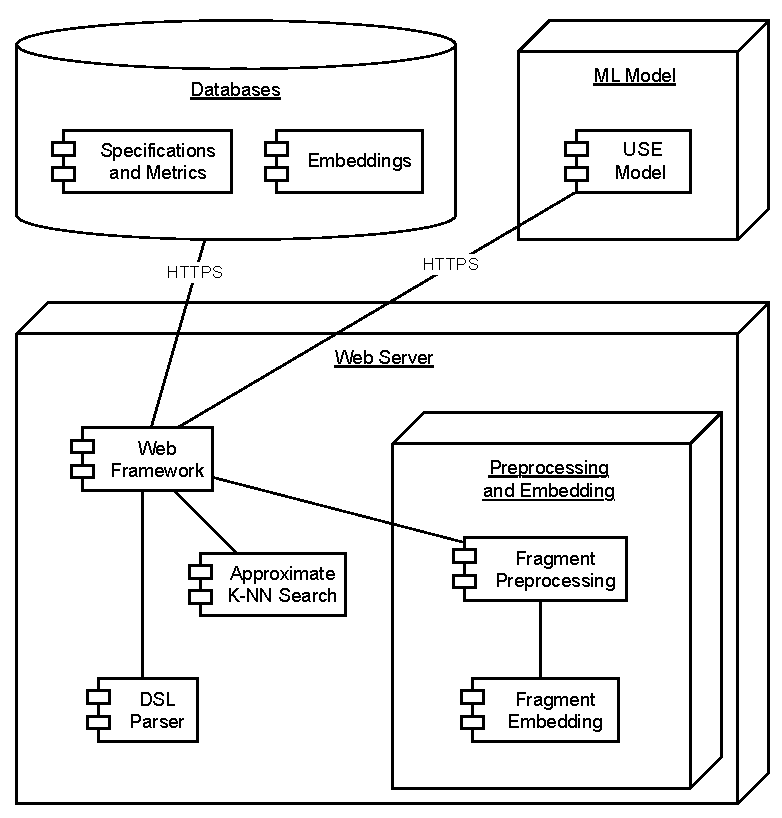
\includegraphics[width=0.55\linewidth]{assets/pdf/architecture/deployment-view}
    \end{center}

    \caption{API Scout's deployment architecture}
    \label{fig:deployment-architecture}
\end{figure}

\section{Databases}\label{sec:databases2}
The two databases -- MongoDB and Elasticsearch -- are contained in two separate Docker containers.
The Docker compose file for these two services is described in Listing~\ref{lst:compose-database}.
Both services do not expose any port to the outside, only in the \verb|backend| Docker network.
In addition, the Elasticsearch instance uses SSL/TLS to enable security when transporting data to and from the database.

\begin{lstlisting}[language=docker-compose,caption={Docker compose for the databases},label={lst:compose-database},captionpos=b]
version: "3.8"
services:
  mongo_db:
    container_name: mongo
    image: mongo:latest
    environment:
      "MONGO_INITDB_ROOT_USERNAME=root"
      "MONGO_INITDB_ROOT_PASSWORD=${MONGO_PASSWORD}"
    volumes:
      - "mongo:/data/db"
    networks:
      - backend

  es_db:
    container_name: es
    image: docker.elastic.co/elasticsearch/elasticsearch:8.12.2
    environment:
      - "node.name=es"
      - "cluster.initial_master_nodes=es"
      - "ELASTIC_PASSWORD=${ELASTIC_PASSWORD}"
      - "ES_JAVA_OPTS=-Xms6000m -Xmx6000m"
      - "xpack.license.self_generated.type=trial"
      - "xpack.security.enabled=true"
      - "xpack.security.http.ssl.enabled=true"
      - "xpack.security.http.ssl.key=${CERTS_DIR}/es/es.key"
      - "xpack.security.http.ssl.certificate_authorities=
          $CERTS_DIR/ca/ca.crt"
      - "xpack.security.http.ssl.certificate=$CERTS_DIR/es/es.crt"
      - "xpack.security.transport.ssl.enabled=true"
      - "xpack.security.transport.ssl.verification_mode=certificate"
      - "xpack.security.transport.ssl.certificate_authorities=
          ${CERTS_DIR}/ca/ca.crt"
      - "xpack.security.transport.ssl.certificate=${CERTS_DIR}/es/es.crt"
      - "xpack.security.transport.ssl.key=${CERTS_DIR}/es/es.key"
    volumes:
      - "data:/usr/share/elasticsearch/data"
      - "certs:${CERTS_DIR}"
    networks:
      - backend

  volumes: { "data", "certs", "mongo" }
  networks:
    backend:
      external: true
\end{lstlisting}

\section{ML Model}\label{sec:ml-model}
The machine learning model used for vector embedding (USE -- Section~\ref{subsec:document-embedding}) is served by a docker image called \verb|tensorflow/serving|.
This image expects a Tensorflow model to be inside the container.
Using this image, it creates several REST endpoints.
The endpoint used by us is the inference endpoint.
We pass a series of fragments as input, and the container will respond with their respective vector embeddings (as explained in Section~\ref{sec:use-model}).
The Docker compose file for this container is described in Listing~\ref{lst:compose-model}.

\begin{lstlisting}[language=docker-compose,caption={Docker compose for the ml model},label={lst:compose-model},captionpos=b]
      version: "3.8"
      services:
        models_ct:
          image: tensorflow/serving
          container_name: models
          environment:
           "MODEL_NAME=universal-encoder"
          volumes:
            - "./models/universal-encoder:/models/universal-encoder"
          networks:
            - backend

      networks:
        backend:
          external: true
\end{lstlisting}

\section{Web Server}\label{sec:web-server}
Finally, we have the Web server container.
This container is based off of a custom Docker image -- described in Listing~\ref{lst:dokerfile} -- in which we build both the Golang application, and the OpenAPI specification -- to create the web documentation for the service.

\begin{lstlisting}[language=docker,caption={Dockerfile for the web server},label={lst:dokerfile},captionpos=b]
           FROM golang:alpine as builder

           WORKDIR /backend

           COPY go.* ./
           RUN go mod download

           COPY . .
           RUN go install github.com/swaggo/swag/cmd/swag@latest
           RUN cd app && swag init
           RUN go build -o /backend/build/app /backend/app

           FROM alpine:latest

           WORKDIR /backend

           ARG GIN_MODE
           ARG MODELS_HOST

           COPY --from=builder /backend/build/app /backend/build/app

           EXPOSE 8080
           ENTRYPOINT [ "/backend/build/app" ]
\end{lstlisting}

\noindent After pushing the Docker image to Docker Hub, we pull it from the server and use the Docker compose document in Listing~\ref{lst:compose-web} to start the service.
Moreover, this is the only service that exposes a port outside the Docker network, namely, port 80.

\begin{lstlisting}[language=docker-compose,caption={Docker compose for the Web server},label={lst:compose-web},captionpos=b]
                   version: "3.8"
                   services:
                     web_server:
                       image: edoriggio/api-scout:dev
                       container_name: backend
                       environment:
                         "GIN_MODE=release"
                         "MODELS_HOST=models"
                       volumes:
                         - ./config:/backend/config
                         - ./ca.crt:/backend/ca.crt
                       networks:
                         - backend
                       ports:
                         - "8080:80"

                   networks:
                     backend:
                       external: true
\end{lstlisting}

\section{CI/CD pipeline}\label{sec:ci-cd-pipeline}
Regarding the Continuous Integration and Continuous Deployment (CI/CD) of the tool, we have implemented a pipeline for it in GitHub using GitHub Actions \footnote{https://docs.github.com/en/actions}.
GitHub Actions allows us to create YML files containing the pipeline we want GitHub to run whenever certain conditions are met.
Our pipeline is described in Listing~\ref{lst:ci-cd-pipeline}.
Now, we will analyze this file more in detail. \\ \\
As we can see at the top of the file (Lines 1--3), we have the name of the pipeline and the trigger.
The trigger, in this case, has been set to \verb|push|.
This means that every time a push event happens in GitHub in this specific repository, then the CI/CD pipeline will start.
Next, we have the jobs performed by the action (Lines 5--61). \\ \\
The first job to be performed is a testing job (Lines 6--32).
In this case, we check out the repo (Lines 9--10), set up the Golang environment (Lines 12--15), install of the dependencies present in the \verb|go.mod| file (Lines 17--20), build the application (Lines 22--23), run the tests using a special testing package (Lines 25--26), and finally export the test results as an artifact (Lines 28--32). \\ \\
The second and last job is a deployment job (Lines 34--61).
This job needs a few more conditions than the previous in order to run.
First of all, the testing pipeline must succeed for the deployment pipeline to run (Line 36).
Moreover, the job will run only if the push event is on either the \verb|main| or \verb|dev| branches.
This was done to avoid deploying unstable branches (Line 37).
Finally, we have the steps.
In this case, GitHub will checkout the repo (Lines 39--40), login into our Docker Hub \footnote{https://hub.docker.com/} account using some repository secrets (Lines 42--46), extract some metadata from the pull event (Lines 48--52), and finally build the Dockerfile and push the image to Docker Hub using the metadata to tag the image (Lines 54--61).

\begin{center}
    \lstset{
        numbers=left,
        firstnumber=1
    }

    \begin{lstlisting}[language=yaml,caption={YML file containing the CI/CD pipeline},label={lst:ci-cd-pipeline},captionpos=b]
      name: Test and Deploy Backend

      on: [ push ]

      jobs:
        test:
          runs-on: "ubuntu-latest"
          steps:
            - name: Checkout repo
              uses: actions/checkout@v4

            - name: Setup golang
              uses: actions/setup-go@v5
              with:
                go-version: "1.22"

            - name: Install dependencies
              run: |
                go install gotest.tools/gotestsum@latest
                go get ./...

            - name: Build
              run: go build -o ./main ./app

            - name: Run tests
              run: gotestsum ./app/tests/... > tests-result.txt

            - name: Upload tests result
              uses: actions/upload-artifact@v4
              with:
                name: tests-result
                path: tests-result.txt

        deploy:
          runs-on: ubuntu-latest
          needs: test
          if: contains("refs/heads/dev, refs/heads/main", github.ref)
          steps:
            - name: Checkout repo
              uses: actions/checkout@v4

            - name: Log in to Docker Hub
              uses: docker/login-action@v3
              with:
                username: ${{ secrets.DOCKER_USERNAME }}
                password: ${{ secrets.DOCKER_PASSWORD }}

            - name: Extract metadata
              id: meta
              uses: docker/metadata-action@v5
              with:
                images: edoriggio/api-scout

            - name: Build and push image
              uses: docker/build-push-action@v5
              with:
                context: .
                file: ./Dockerfile
                push: true
                tags: ${{ steps.meta.outputs.tags }}
                labels: ${{ steps.meta.outputs.labels }}
    \end{lstlisting}
\end{center}

\noindent Figure~\ref{fig:deployment-example} shows an example of a Docker image published to Docker Hub by our pipeline.
As we can see in this example, the image has been tagged \verb|:dev|.
This is because the pipeline was triggered on a push event on the \verb|dev| branch.
To pull the Docker image, one can run the command \verb|docker pull edoriggio/api-scou| \verb|t:dev|, or simply run \verb|docker-compose up -d| on the backend Docker compose file  (Section~\ref{sec:web-framework-1}).

\begin{figure}[h]
    \begin{center}
        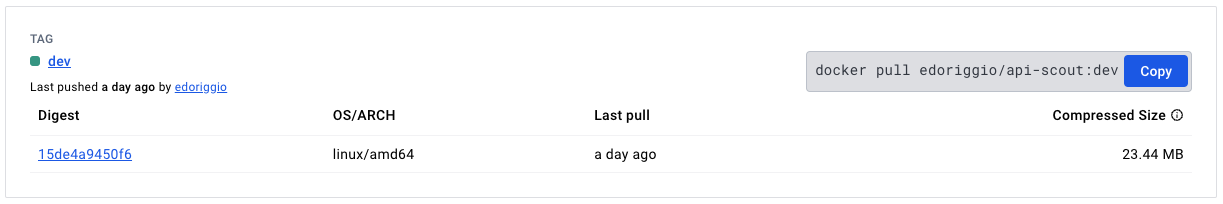
\includegraphics[width=0.9\linewidth]{assets/png/deployment/dev-deployment}
    \end{center}

    \caption{Example of a published Docker image}
    \label{fig:deployment-example}
\end{figure}


    %%%%%%%%%%%%%%%%%%%%%%%%%%%%%%%%%%%%%%%%%%%%%%%%%%%%%%%%%%%%%%%%%
    %%%	EVALUATION %%%%%%%%%%%%%%%%%%%%%%%%%%%%%%%%%%%%%%%%%%%%%%%%%%
    %%%%%%%%%%%%%%%%%%%%%%%%%%%%%%%%%%%%%%%%%%%%%%%%%%%%%%%%%%%%%%%%%

    \chapter{Evaluation}\label{ch:evaluation}

\section{Retrieval Performance}\label{sec:retrieval-performance}
In the following sections, we are going to describe the methods and present the results of the experiments we used to assess the performance of the system.
In this first part of the evaluation, we used several different formulas to evaluate the system.
Moreover, we carried out two different types of experiments to test several different aspects of our information retrieval system.

\subsection{Needles in a Haystack}\label{subsec:needles-in-a-haystack}
In this first batch of experiments, we wanted to test the accuracy of the system's document retrieval.
Since the system contains almost one million documents (the haystack), it is very difficult to know the precise number of relevant documents for each user query -- the number of relevant documents is needed for the computation of both the recall and the F1 score (Section~\ref{subsec:evaluation-methods}).
For this reason, we decided to imagine four different queries, and for each one of them, we created four different API specifications (the needles).
By doing so, we know the number of relevant documents per query -- four in this case -- and we can check how many the system is able to retrieve. \\ \\
Initially, we ran this experiment on four different queries, and for each query, we used ChatGPT 3.5 \footnote{https://chatgpt.com/} to help us generate valid random API specifications related to that query.
The generated specifications can be found in our repository \footnote{https://github.com/APIScout/evaluation} in the \verb|needles| directory.
The result of this experiment can be found in Figure~\ref{fig:nh-1}.
In Table~\ref{tab:metrics-prf}, we have the overall score for each metric (Equation~\ref{eq:overall}) for each $@K$.

\begin{table}[!h]
    \begin{center}
        \begin{tabular}{l c c c c c c c c c c}
            \hline
            \textbf{Metric} & \textbf{@1} & \textbf{@2} & \textbf{@3} & \textbf{@4} & \textbf{@5} & \textbf{@6} & \textbf{@7} & \textbf{@8} & \textbf{@9} & \textbf{@10} \\ \hline
            $\overline{\text{Precision}}$ & 1.0 & 1.0 & 1.0 & 0.81 & 0.65 & 0.58 & 0.5 & 0.47 & 0.42 & 0.37 \\
            $\overline{\text{Recall}}$ & 0.25 & 0.5 & 0.75 & 0.81 & 0.81 & 0.87 & 0.87 & 0.94 & 0.93 & 0.93 \\
            $\overline{\text{F1 Score}}$ & 0.4 & 0.67 & 0.86 & 0.81 & 0.72 & 0.7 & 0.64 & 0.65 & 0.58 & 0.53 \\ \hline
        \end{tabular}
    \end{center}

    \caption{Mean score for each metric $@K$ for Figure~\ref{fig:nh-1}}
    \label{tab:metrics-prf}
\end{table}

\noindent In addition to this experiment, we also tried to see if the length of the query would impact the retrieval performance of the system.
To test this, we took the query -- for example \("\)weather forecast service\("\) -- and created four sub-queries.
The generated sub-queries would be, in this case, \("\)weather\("\), \("\)weather forecast\("\), and \("\)weather forecast service\("\).
The fourth one, however, is a random substring taken from one of the natural language tags of the specification.
For example, \("\)the API returns the next 4 days of weather forecasts\("\).
This second experiment using subqueries was done on each one of the original four queries, generating the graphs in Figures~\ref{fig:nh-2},~\ref{fig:nh-3},~\ref{fig:nh-4}, and~\ref{fig:nh-5}.
In addition to these graphs, we have also generated a t-SNE plot (Section~\ref{subsec:t-sne-plots}) for each group of subqueries.
These plots can be found in Figures~\ref{fig:tsne-2},~\ref{fig:tsne-3},~\ref{fig:tsne-4}, and~\ref{fig:tsne-5}.

\begin{figure}[!h]
    \begin{center}
        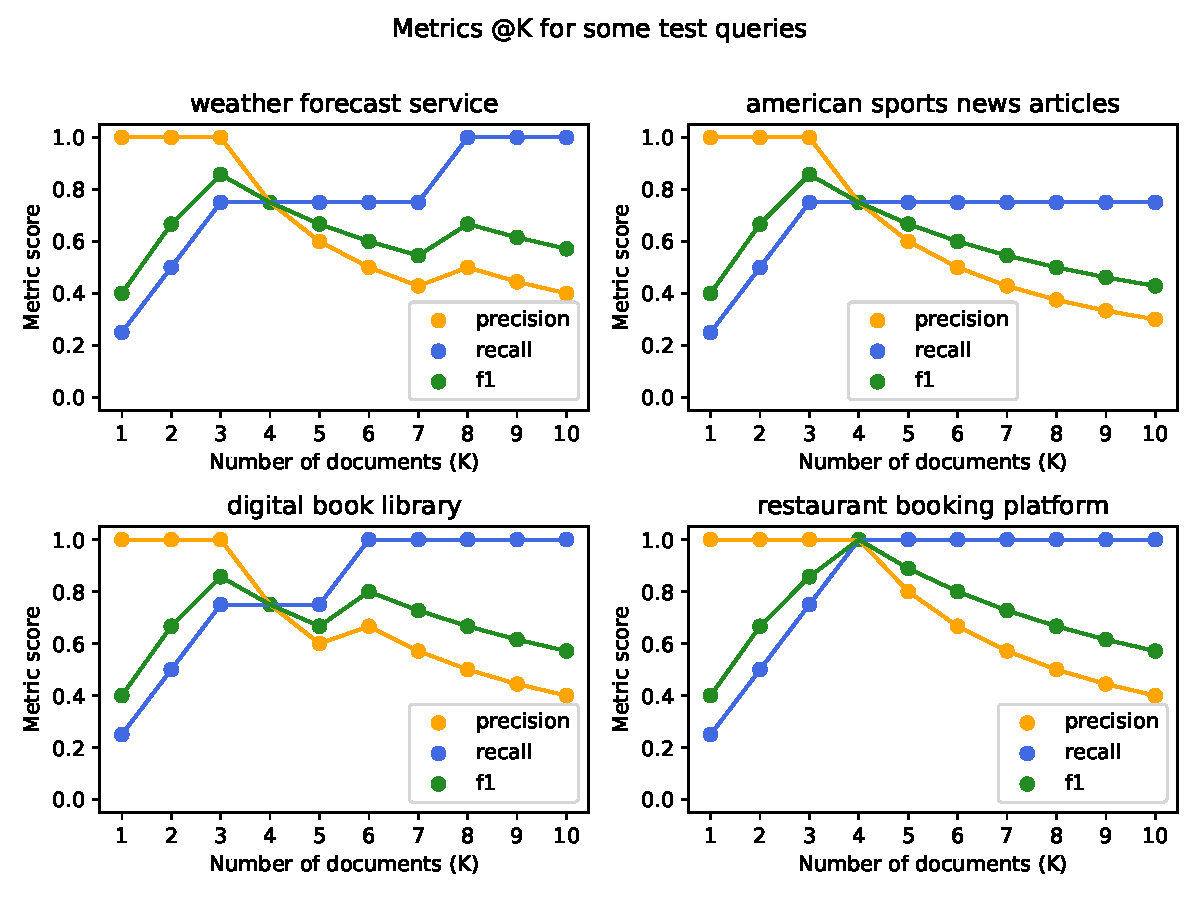
\includegraphics[width=0.8\linewidth]{assets/pdf/evaluation/prec-rec-queries}
    \end{center}

    \caption{Needles in a haystack experiment on four random queries}
    \label{fig:nh-1}
\end{figure}

\noindent To further analyze the results of this batch of experiments, we would like to understand if a high value of the parameter $K$ and a small query containing only keywords are causally related to a high recall. \\ \\
To verify this causation, we first need to define all of its nodes.
Since we are dealing with four \("\)needles\("\) (inserted documents), we define a high $K$ to be $K\geq3$ and the precision to be $P\geq0.75$.
Finally, we define a small query to have a number of words $w$ to be $w\leq4$.
Moreover, in this last case, we consider $K$ to be 10.
From all these elements, we can build our causal graph (Figure~\ref{fig:dag-1}).

\begin{figure}[!h]
    \begin{center}
        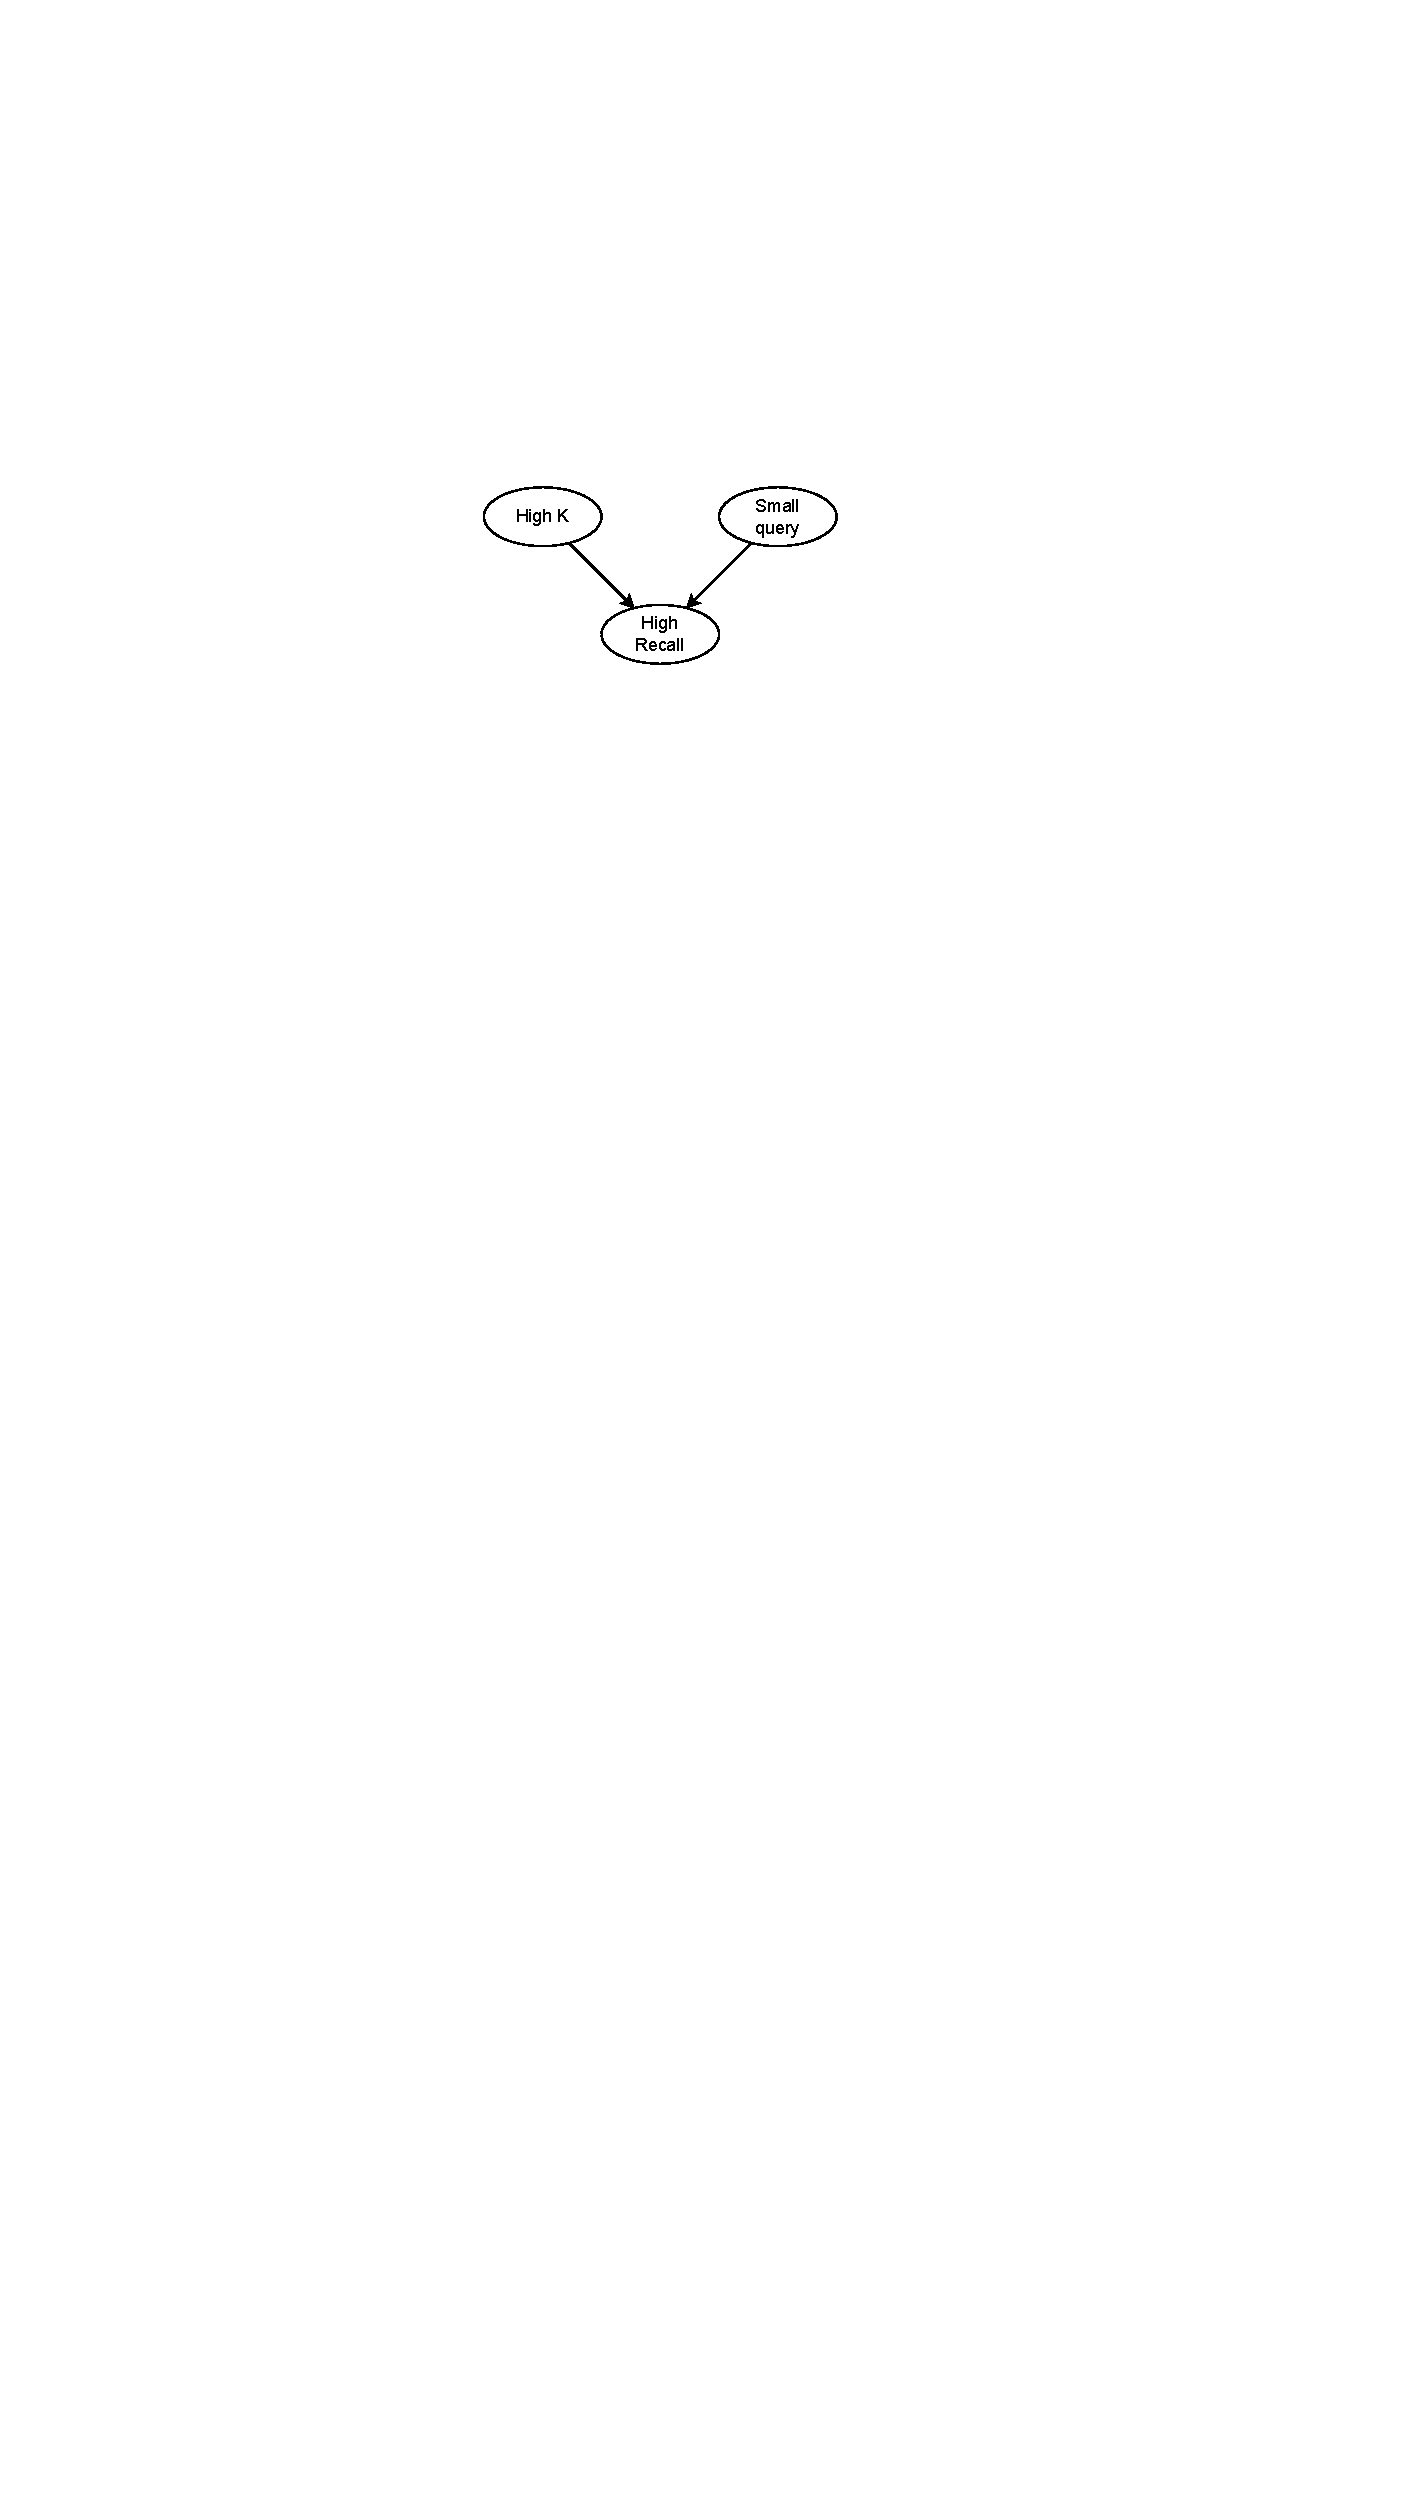
\includegraphics[width=0.3\linewidth]{assets/pdf/evaluation/dag-rec}
    \end{center}

    \caption{Causal graph}
    \label{fig:dag-1}
\end{figure}

\noindent Now that we have built the causal graph, we would like to compute the probability that each relation (an edge in the graph) is a causal relation.
To do so, we define that the probability must be computed by using Equation~\ref{eq:prob}.

\begin{equation}
    P_i = \frac{\text{Cases matching the restrictions}}{\text{Cases that should match the restrictions}}
    \label{eq:prob}
\end{equation}

\noindent With the probability formula defined, we can now proceed to compute the probabilities for each path.
In the case of the path $\text{High $K$} \rightarrow \text{High Recall}$, we have a probability of:
\[P_1 = \frac{14}{20} = 0.7\]
In the case of the path $\text{Small Query} \rightarrow \text{High Recall}$, we have a probability of:
\[P_2 = \frac{15}{16} = 0.9\]
The final causal graph can be found in Figure~\ref{fig:rec-probs}.
In this graph, we can see that there are very high probabilities that a high value of $K$ or a small query will lead to a high recall.

\begin{figure}[!h]
    \begin{center}
        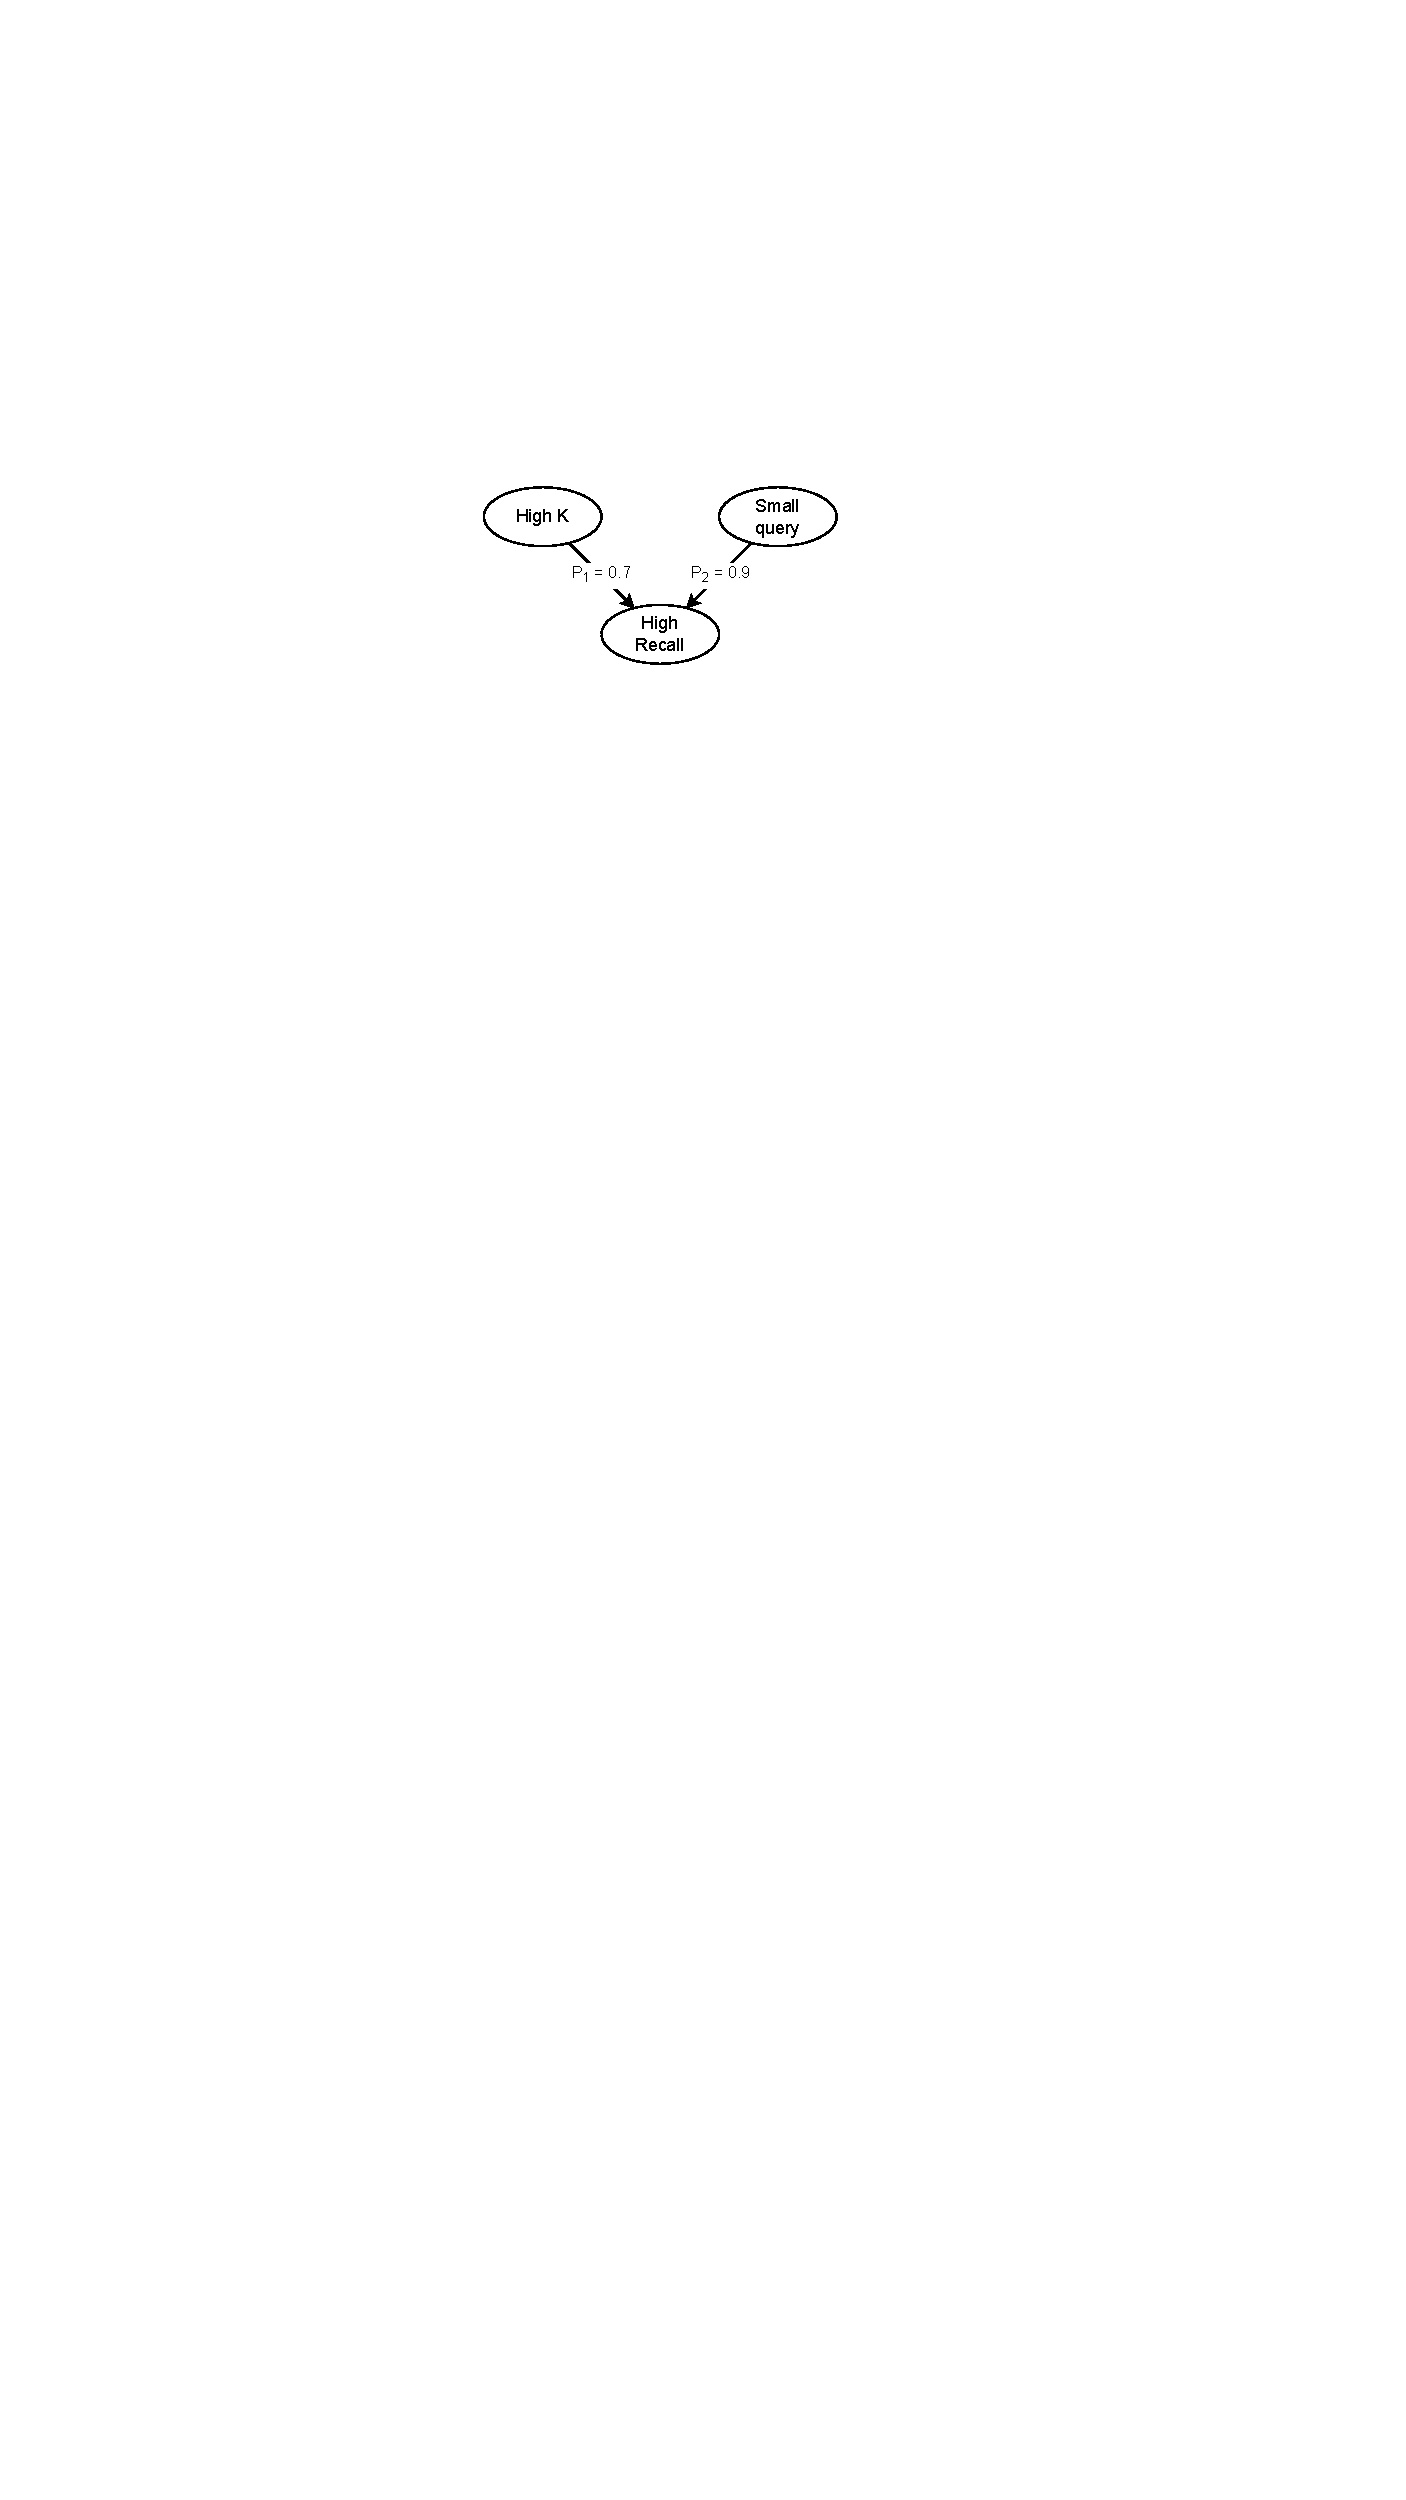
\includegraphics[width=0.3\linewidth]{assets/pdf/evaluation/dag-rec-probs}
    \end{center}

    \caption{Causal graph with probabilities}
    \label{fig:rec-probs}
\end{figure}

% ===========================================
% ===========================================

\begin{figure}[!h]
    \begin{center}
        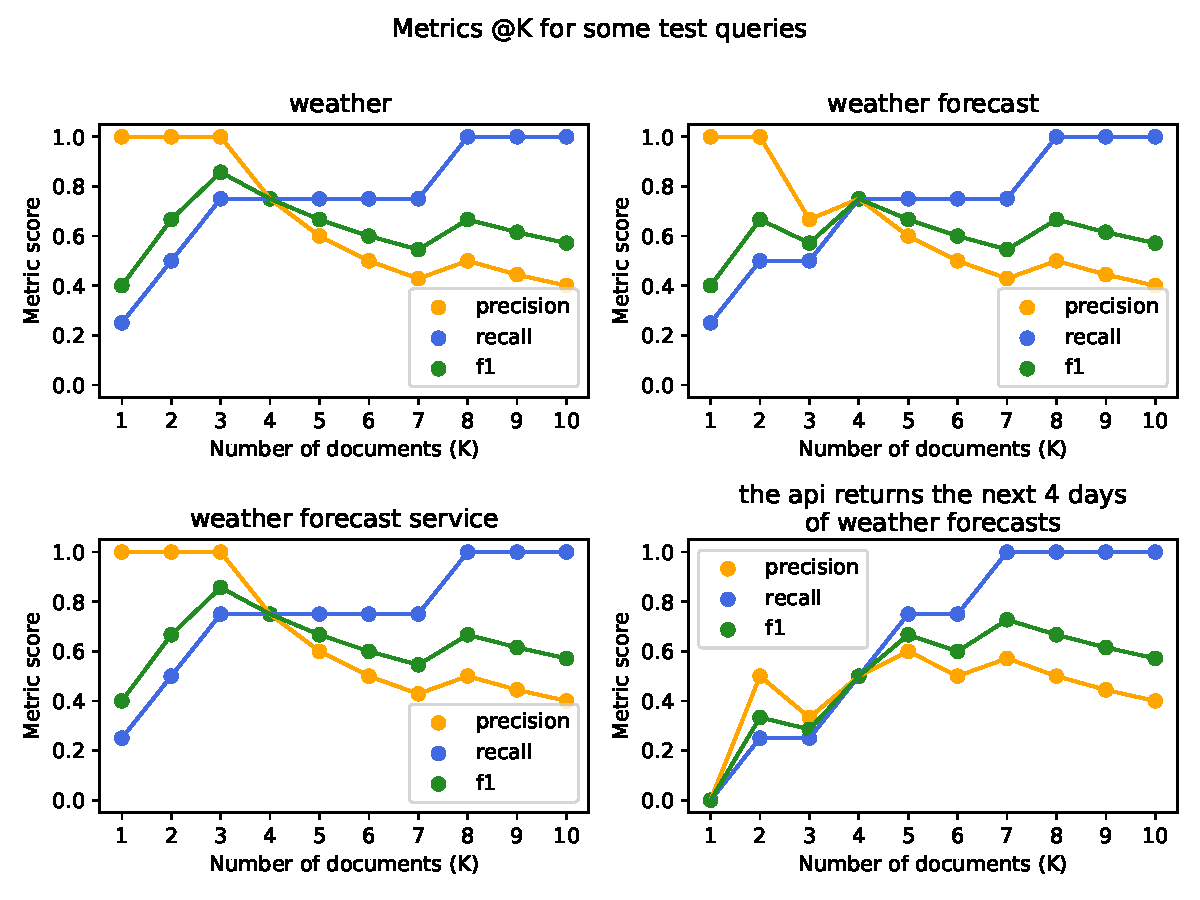
\includegraphics[width=0.8\linewidth]{assets/pdf/evaluation/prec-rec-weather}
    \end{center}

    \caption{Needles in a haystack experiment on different length queries related to weather forecast}
    \label{fig:nh-2}
\end{figure}

\begin{figure}[!h]
    \begin{center}
        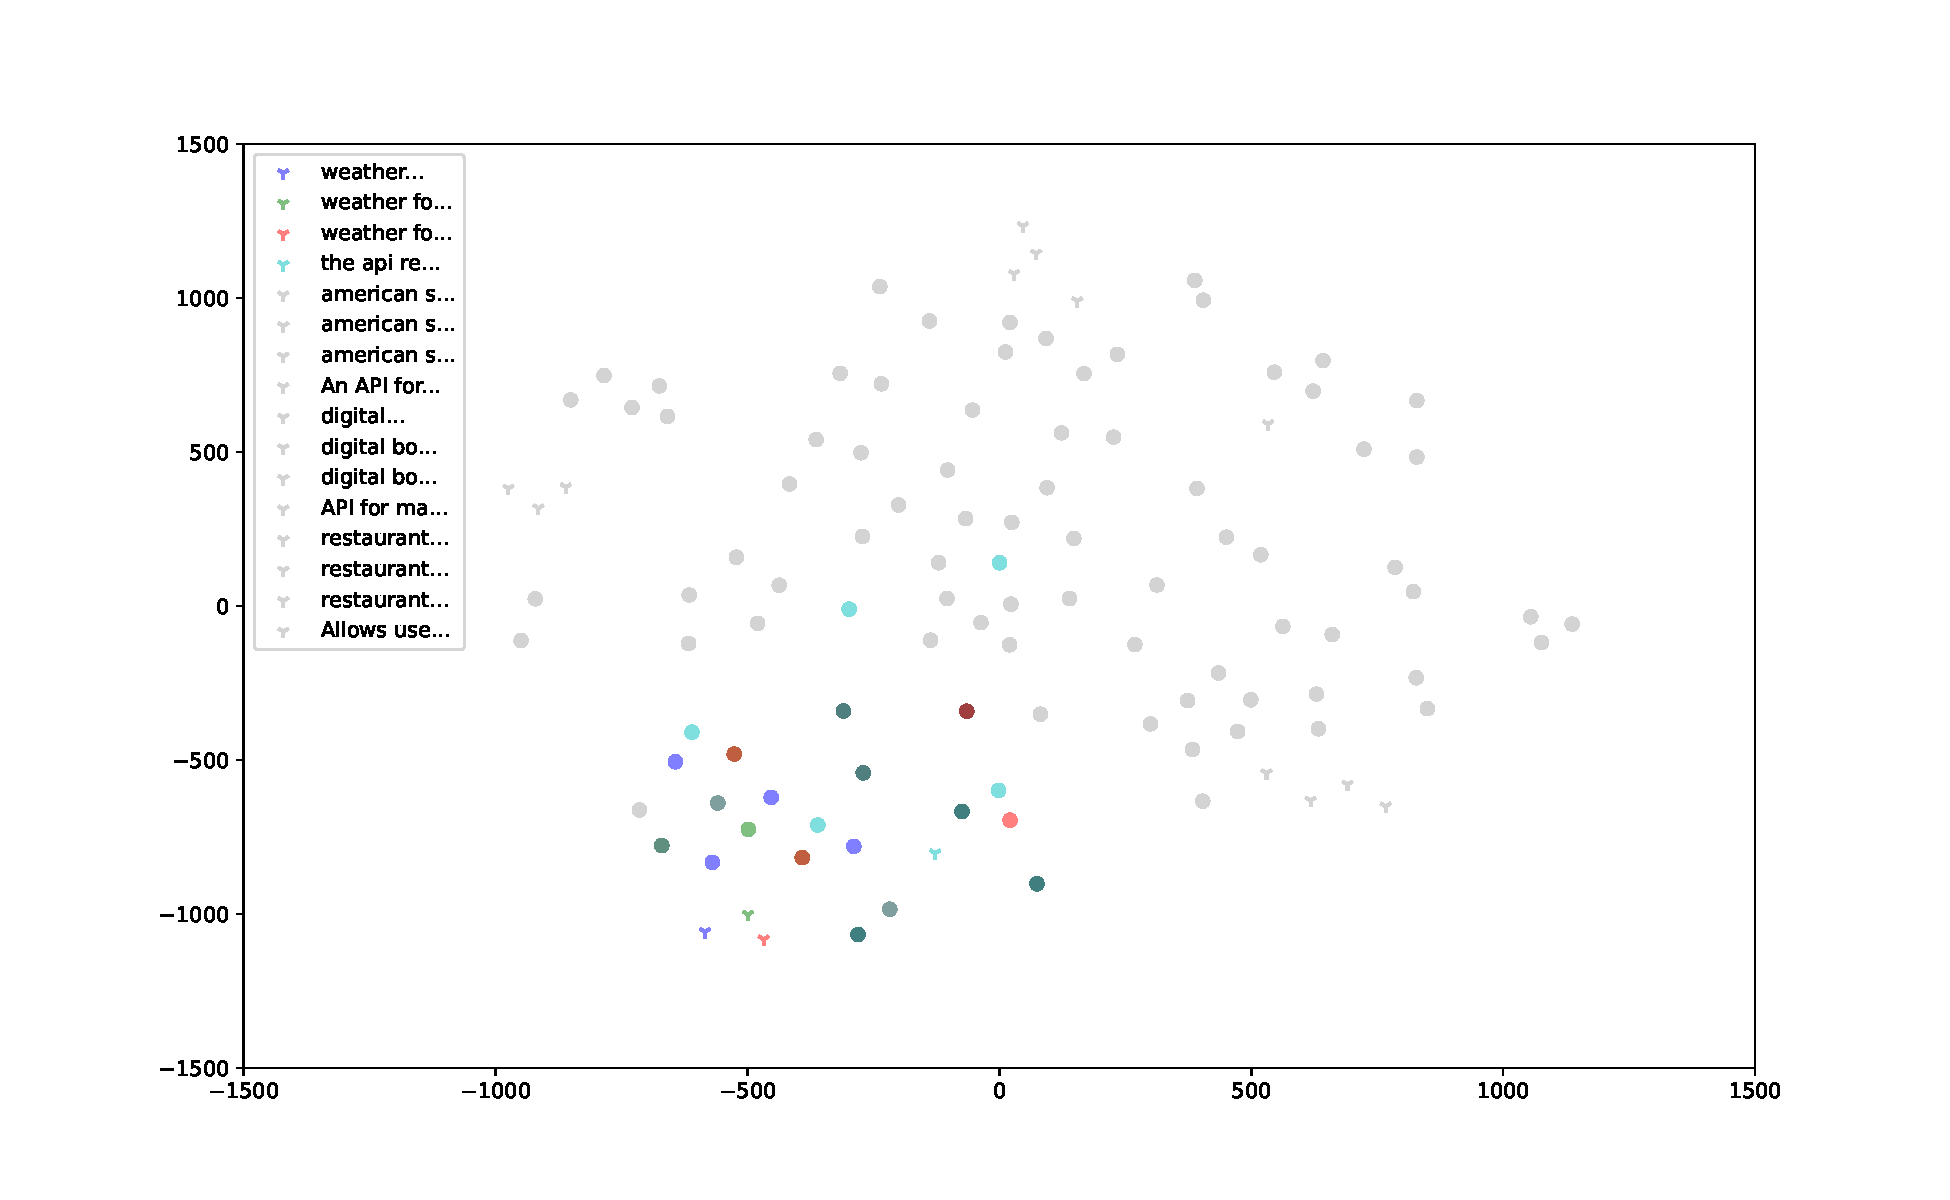
\includegraphics[width=0.8\linewidth]{assets/pdf/evaluation/tsne-weather}
    \end{center}

    \caption{t-SNE graph for the weather forecast queries}
    \label{fig:tsne-2}
\end{figure}

% ===========================================
% ===========================================

\begin{figure}[!h]
    \begin{center}
        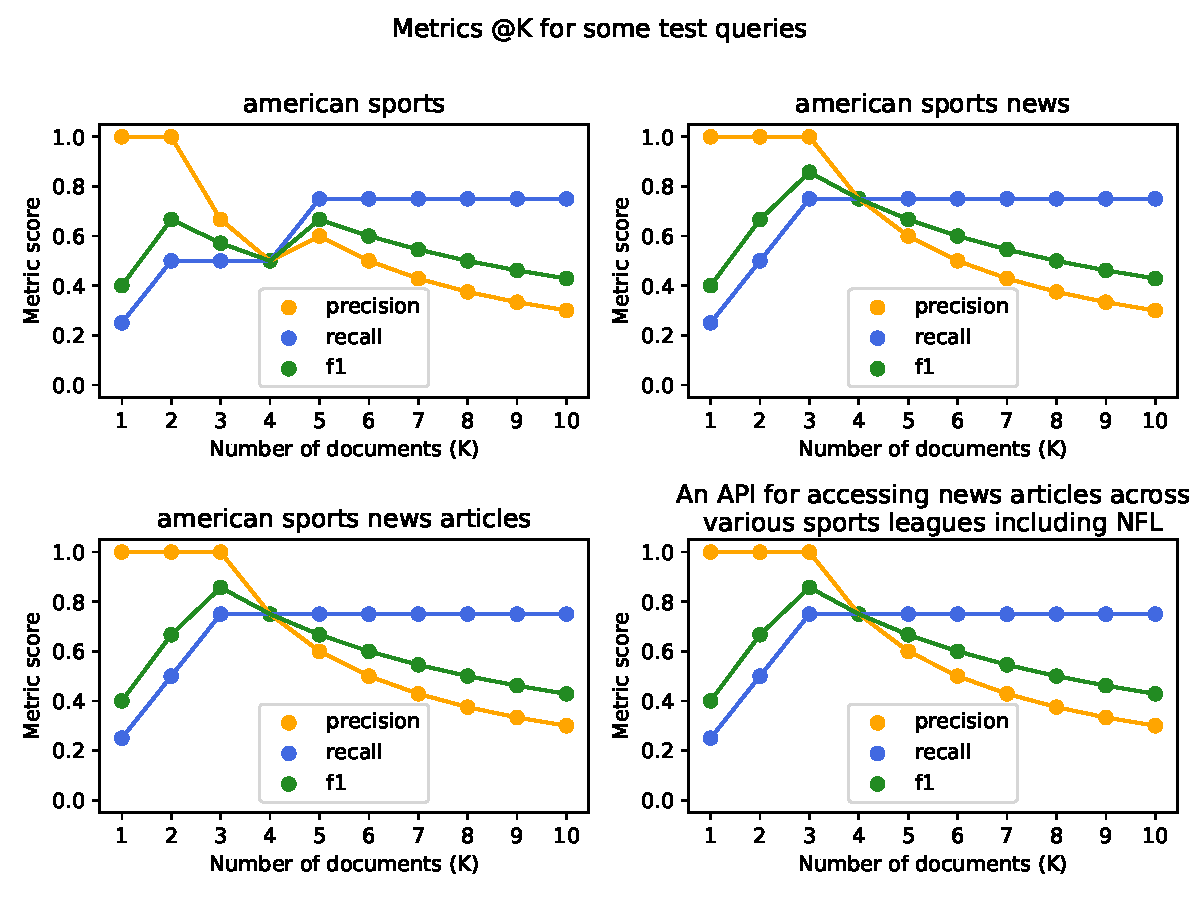
\includegraphics[width=0.8\linewidth]{assets/pdf/evaluation/prec-rec-sports}
    \end{center}

    \caption{Needles in a haystack experiment on different length queries related to American sports}
    \label{fig:nh-3}
\end{figure}

\begin{figure}[!h]
    \begin{center}
        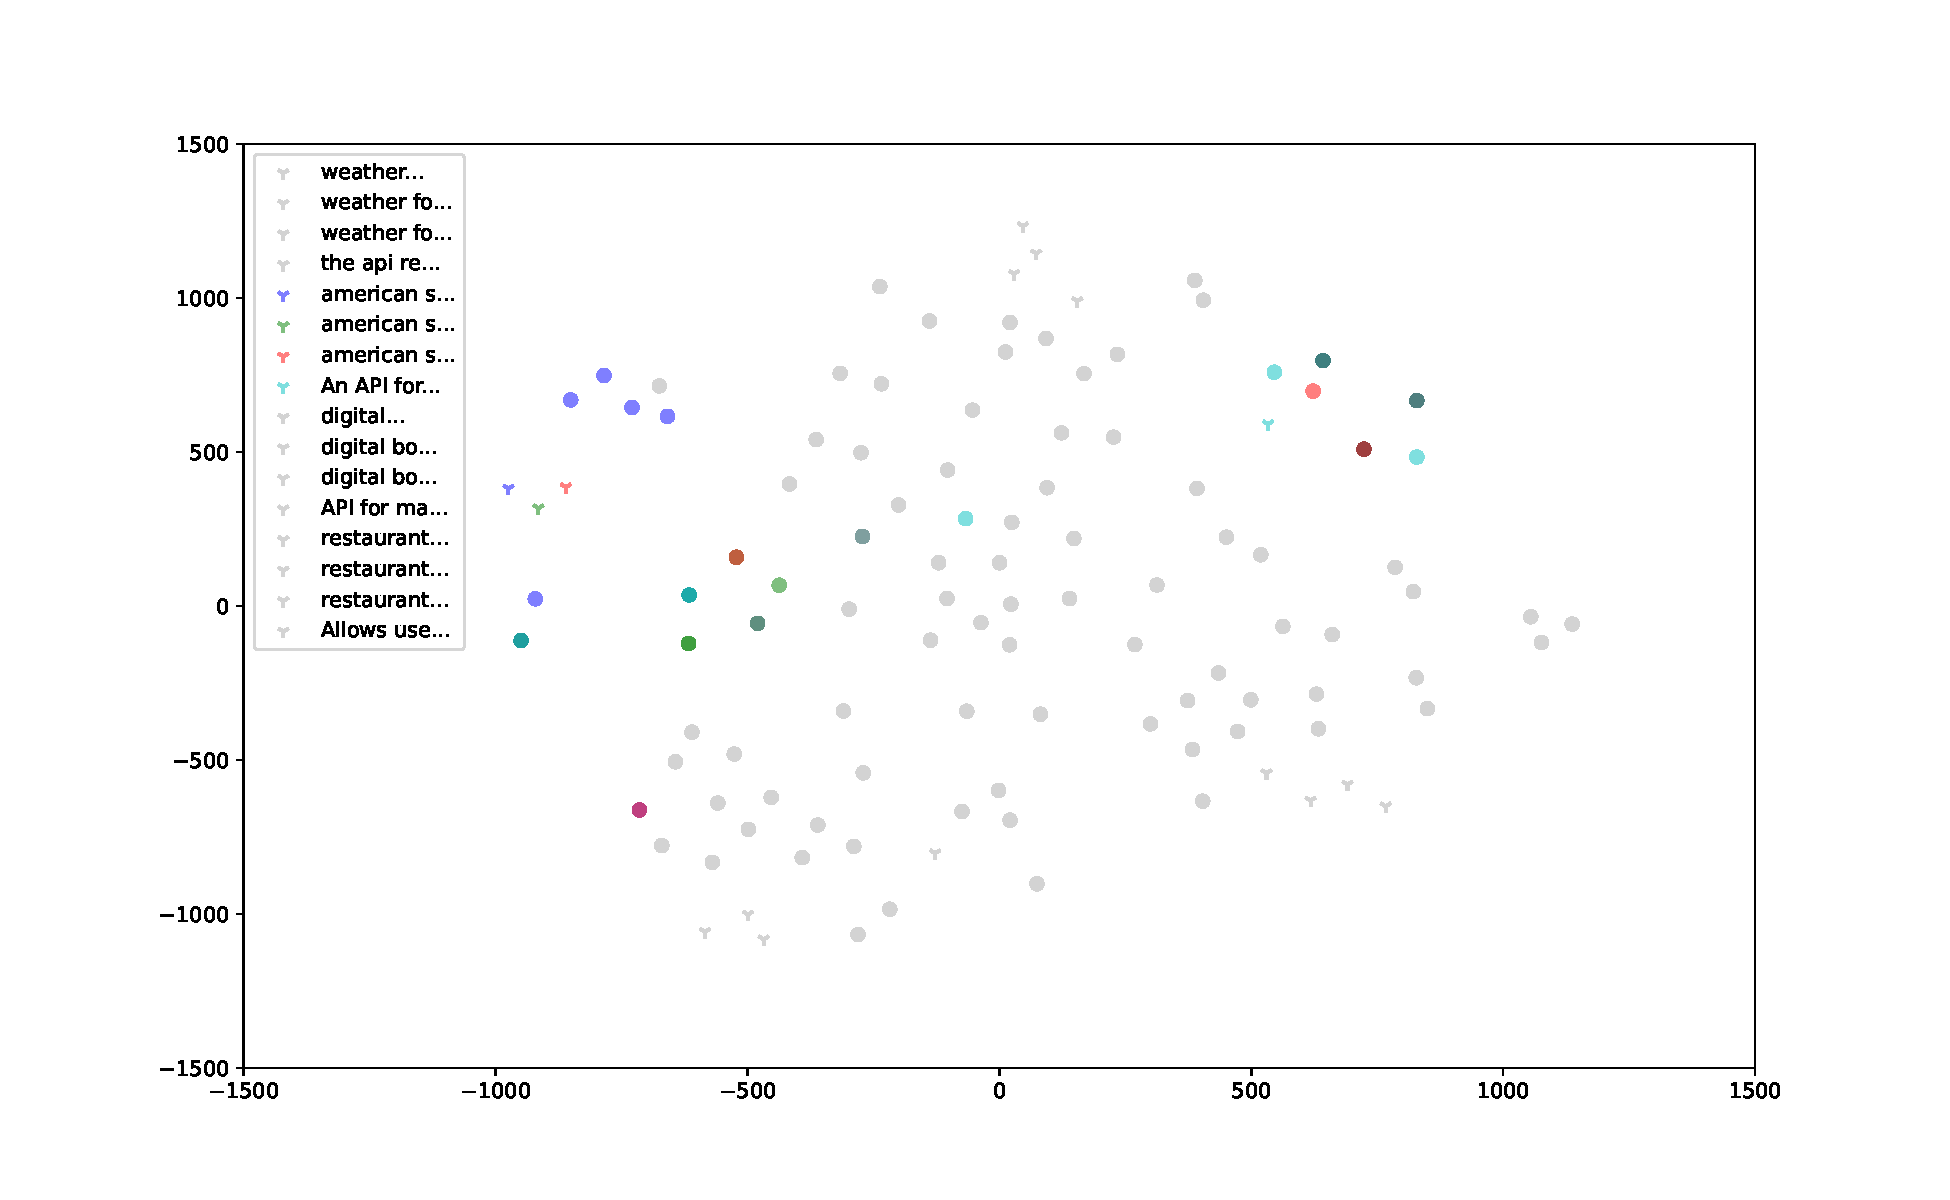
\includegraphics[width=0.8\linewidth]{assets/pdf/evaluation/tsne-sports}
    \end{center}

    \caption{t-SNE graph for the American sports queries}
    \label{fig:tsne-3}
\end{figure}

% ===========================================
% ===========================================

\begin{figure}[!h]
    \begin{center}
        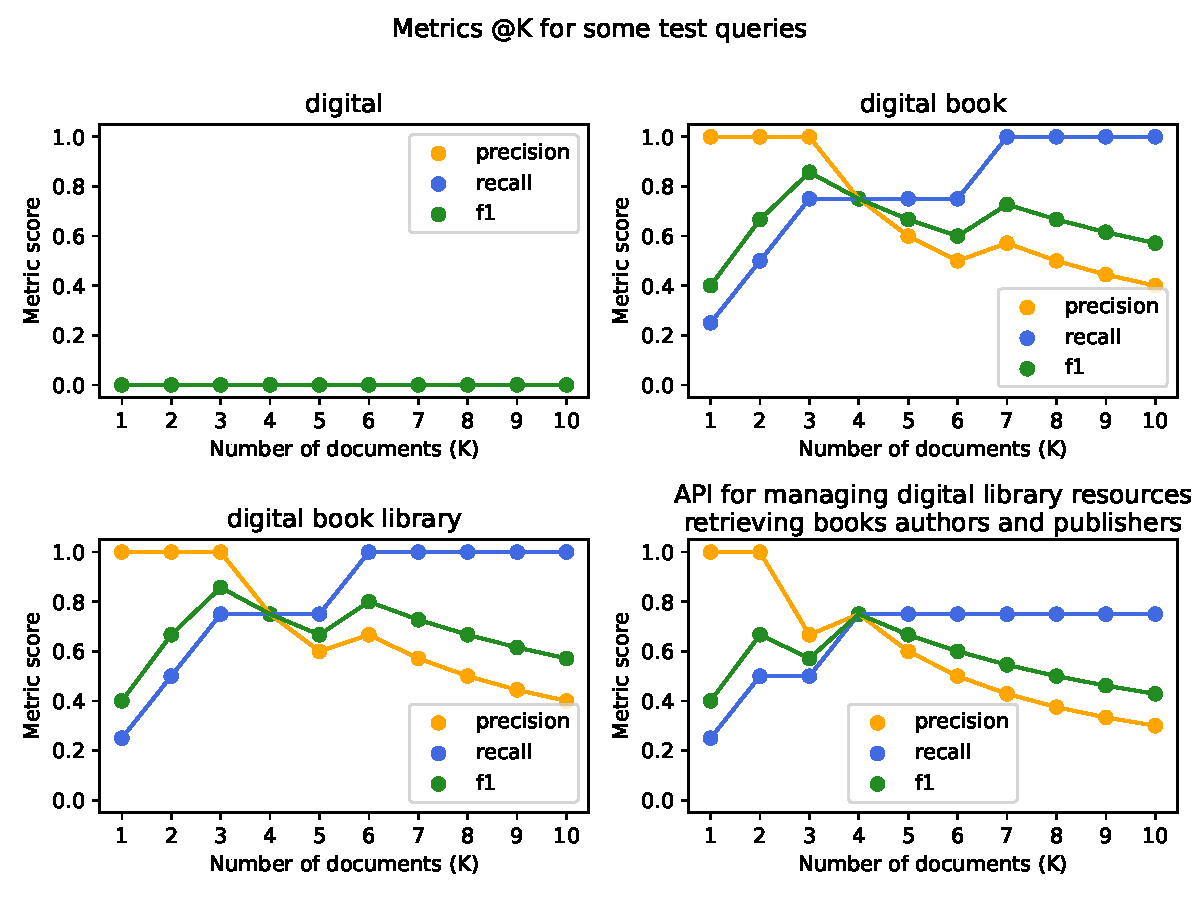
\includegraphics[width=0.8\linewidth]{assets/pdf/evaluation/prec-rec-library}
    \end{center}

    \caption{Needles in a haystack experiment on different length queries related to digital book libraries}
    \label{fig:nh-4}
\end{figure}

\begin{figure}[!h]
    \begin{center}
        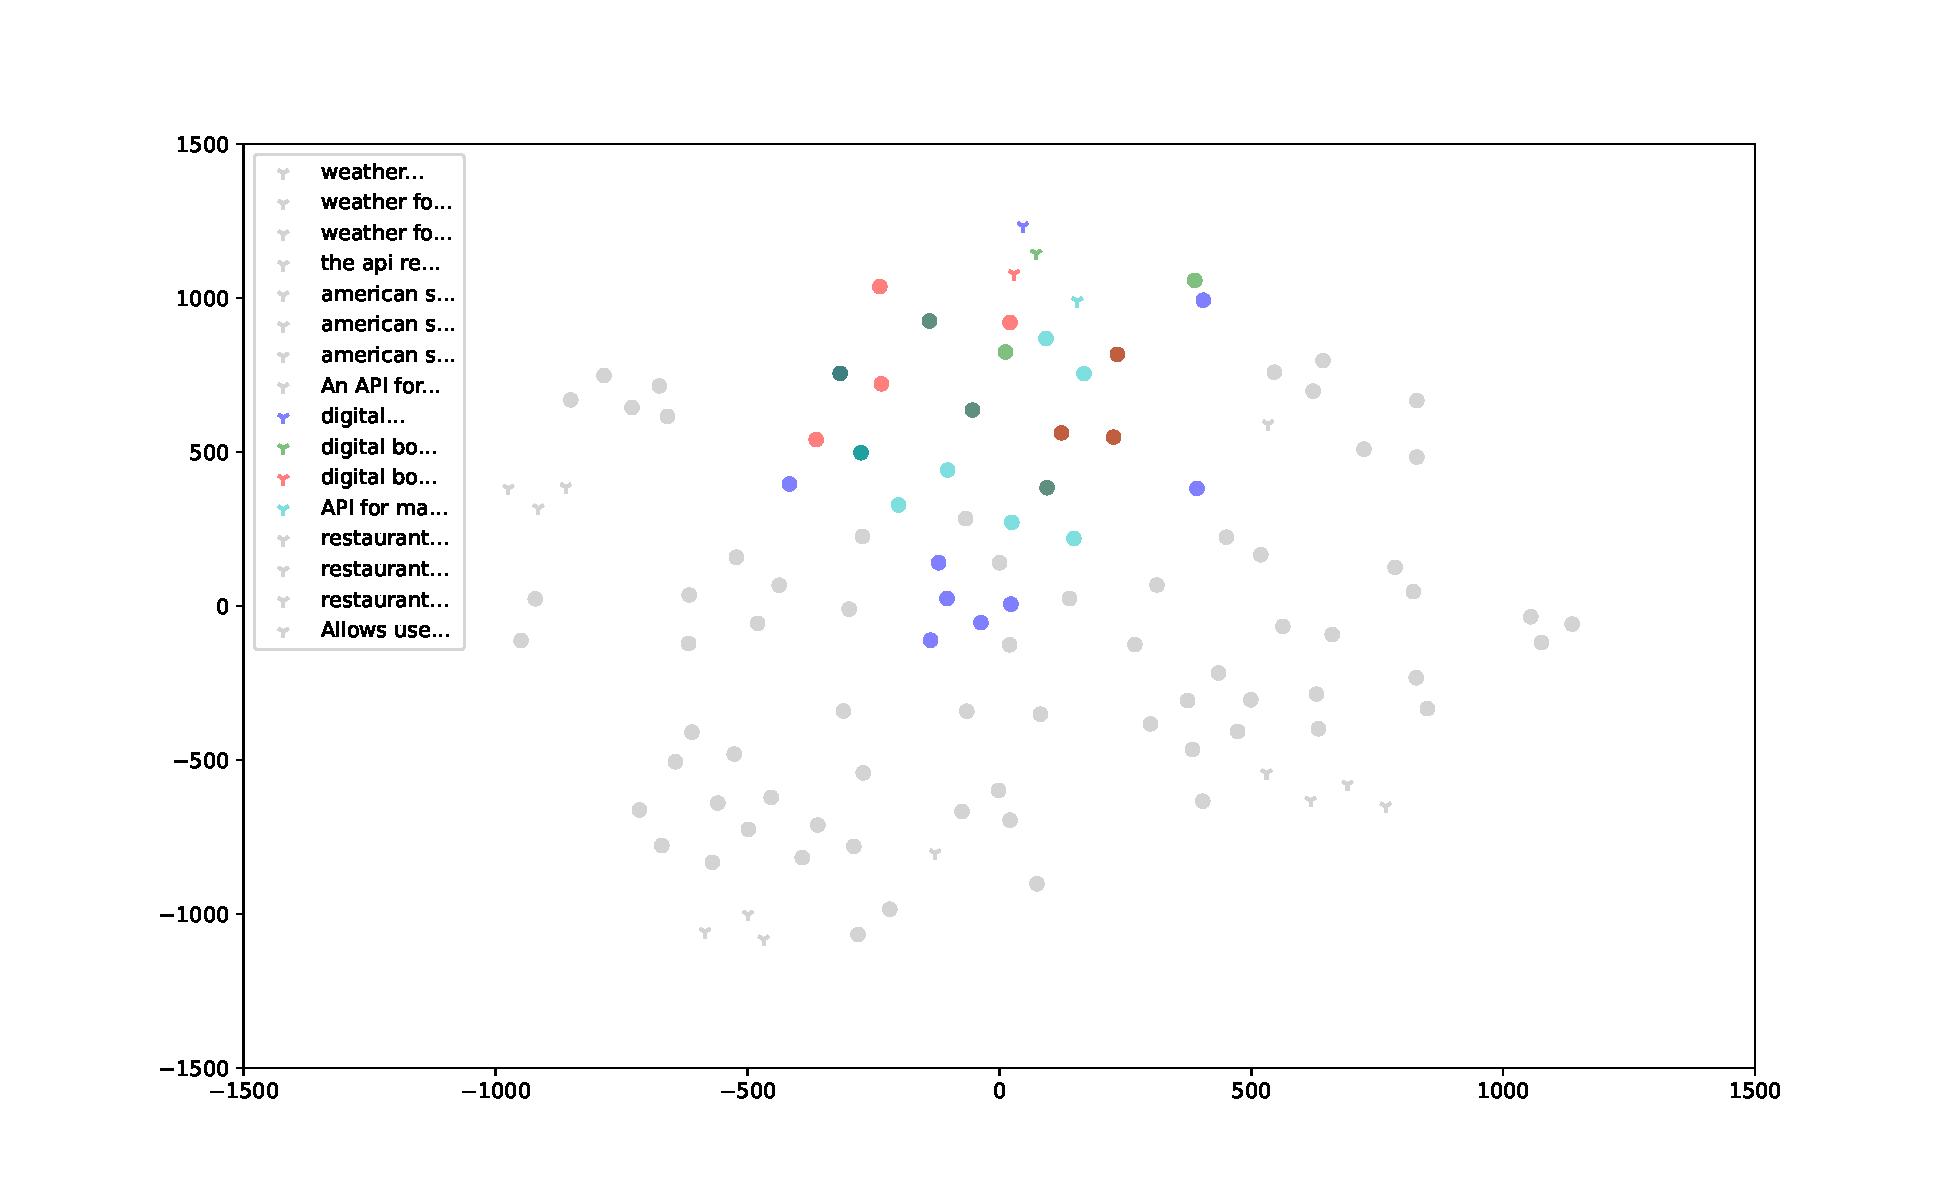
\includegraphics[width=0.8\linewidth]{assets/pdf/evaluation/tsne-books}
    \end{center}

    \caption{t-SNE graph for the digital book libraries queries}
    \label{fig:tsne-4}
\end{figure}

% ===========================================
% ===========================================

\begin{figure}[!h]
    \begin{center}
        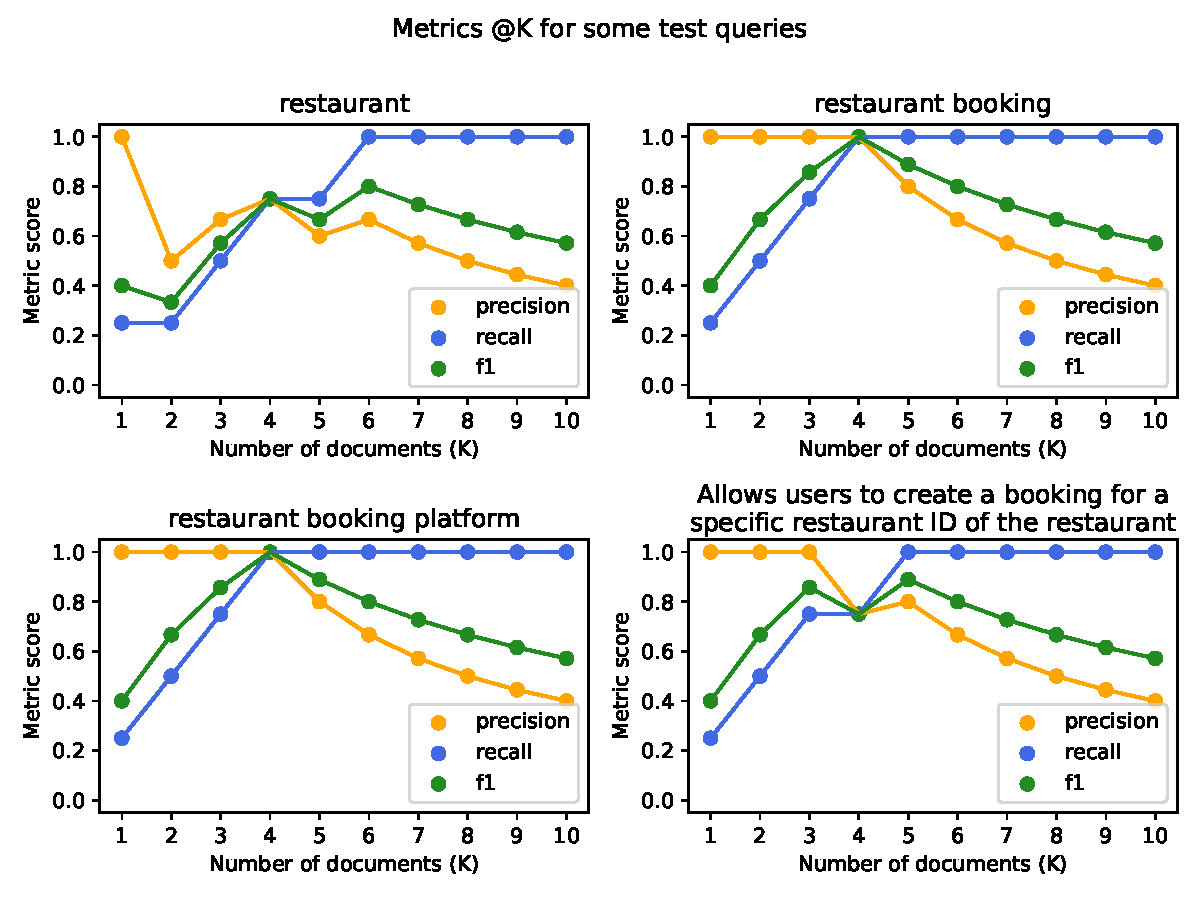
\includegraphics[width=0.8\linewidth]{assets/pdf/evaluation/prec-rec-restaurant}
    \end{center}

    \caption{Needles in a haystack experiment on different length queries related to restaurant bookings}
    \label{fig:nh-5}
\end{figure}

\begin{figure}[!h]
    \begin{center}
        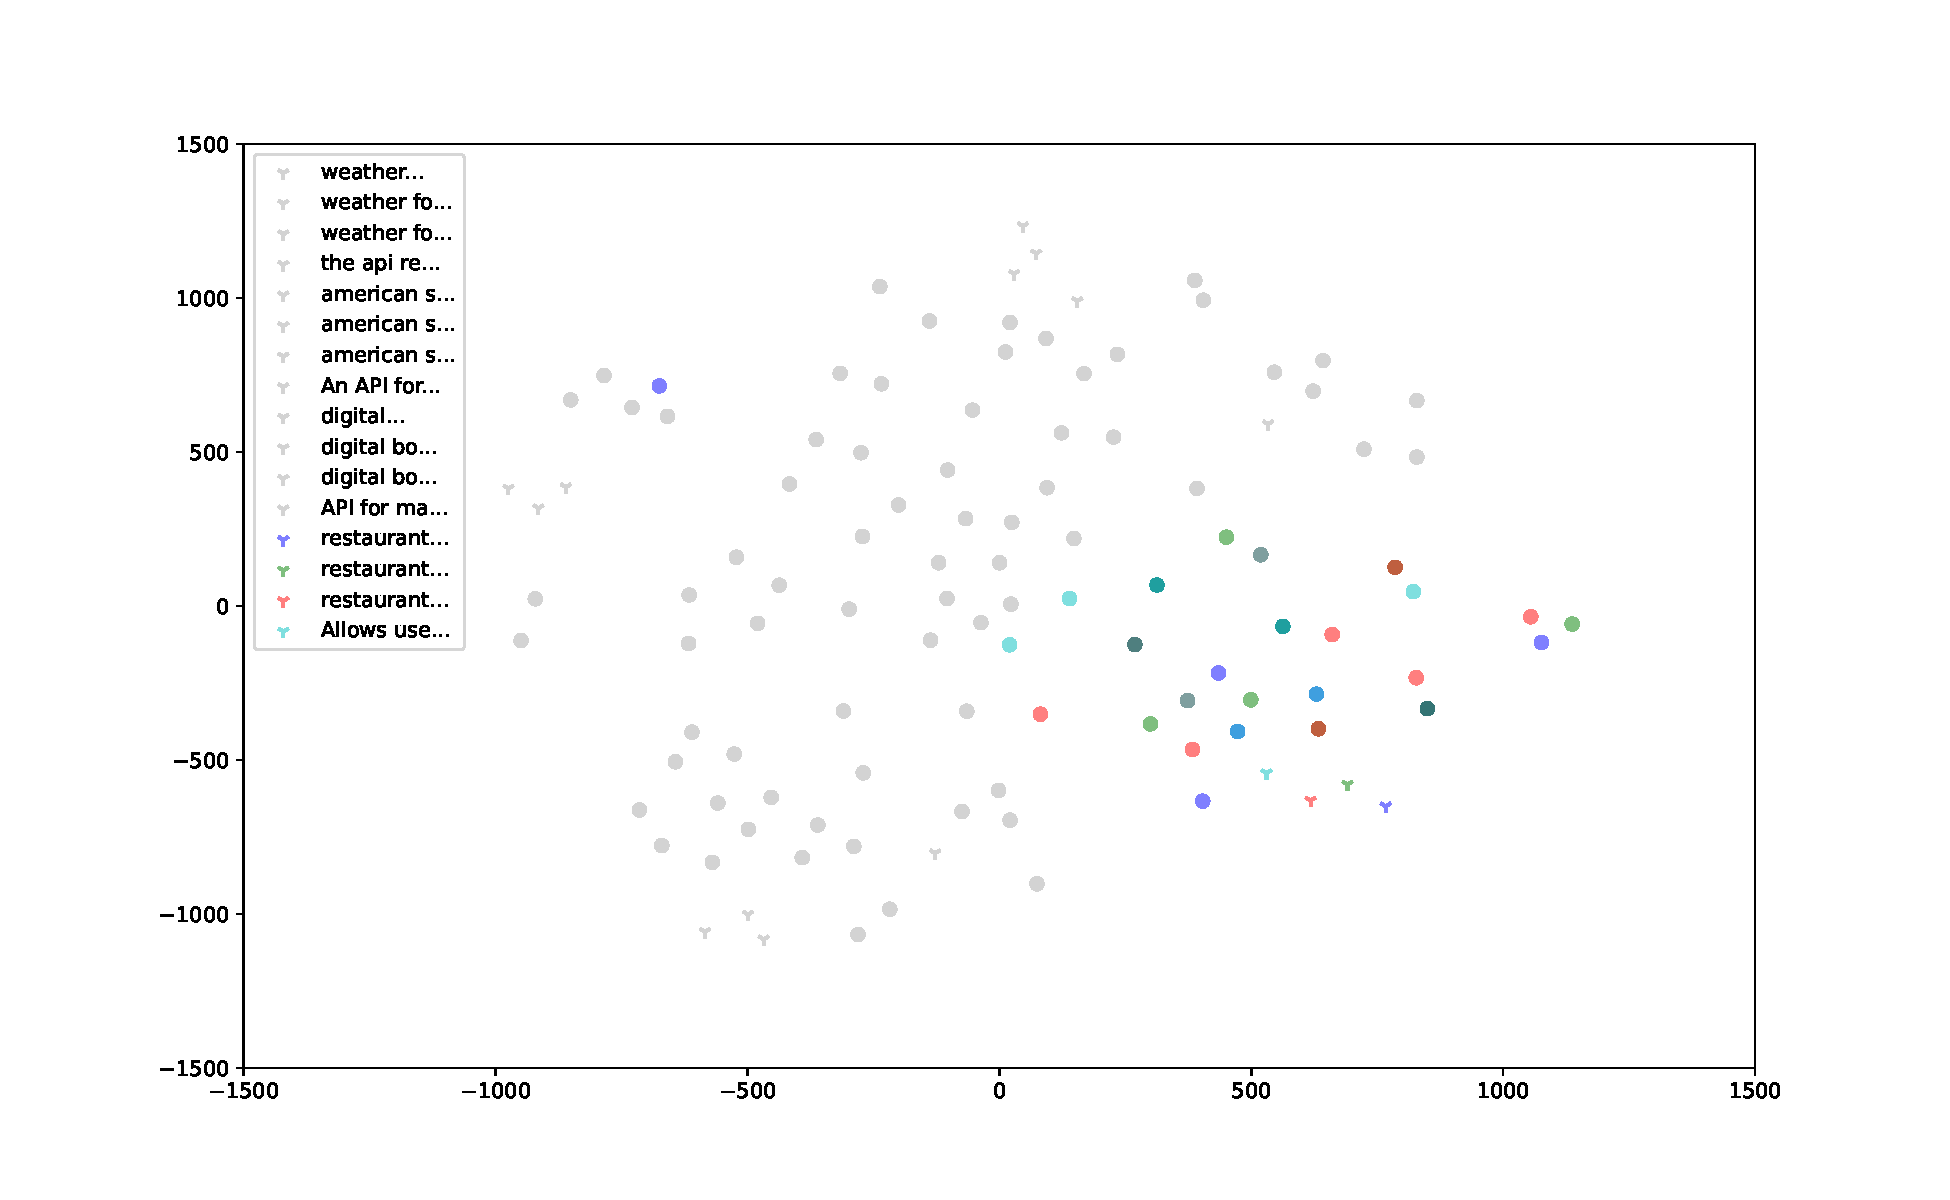
\includegraphics[width=0.8\linewidth]{assets/pdf/evaluation/tsne-restaurant}
    \end{center}

    \caption{t-SNE graph for the restaurant booking queries}
    \label{fig:tsne-5}
\end{figure}

% ===========================================
% ===========================================

\subsection{Overall Retrieval Performance}\label{subsec:overall-retrieval-performance}
In this next experiment, we used the average precision (Equation~\ref{eq:ap}) and precision to evaluate the overall performance of the system -- in this case, we are not considering the \("\)needles\("\) inserted in the previous batch of experiments. \\ \\
To compute the average precision, we need a parameter called $rel_k$ for each retrieved document.
This parameter is binary and indicates whether the document is relevant to the query or not.
Thus, for each query, we went through the first ten results and gave each one a $rel_k$ of 1 or 0.
Now that we know if a document is relevant to the query or not, we can compute the average precision at each $@K$. \\ \\
Moreover, since we now know which document is relevant and which is not, we can also compute the precision.
This is done by counting the number of relevant documents in the top ten and then dividing this number by $K$.
The results of this experiment can be found in Figure~\ref{fig:ap}.
Table~\ref{tab:metrics-pap}, instead, displays the mean average precision (Equation~\ref{eq:map}) and the overall precision for each $@K$. \\ \\
From these results, we can again build a causal graph where we have as nodes a low $K$ and a high precision.
We define a low $K$ to be $K\leq5$, while a high precision to be $P\geq0.6$.
With this causal graph, we want to see whether the first documents returned by the system are relevant or not.
As before, we use Equation~\ref{eq:prob} to compute each edge's probability.
In this case, we only need to compute the probability for path $\text{Low $K$} \rightarrow \text{High Precision}$:
\[P_1 = \frac{3}{4} = 0.75\]
The causal graph is represented in Figure~\ref{fig:dag-prec}.
In this causal graph, we can see that there is a high probability that a low value of $K$ will lead to a high precision, which is one of the main goals of a good retrieval system. \\ \\
In addition to the causal graph, in Figure~\ref{fig:es-scores}, we have plotted how the similarity score returned by Elasticsearch -- that goes from 0 to 1 -- changes for each retrieved document.
As we can see with the values for precision and average precision, the score returned by Elasticsearch drops in a similar way.

\begin{table}[!h]
    \begin{center}
        \begin{tabular}{l c c c c c c c c c c}
            \hline
            \textbf{Metric} & \textbf{@1} & \textbf{@2} & \textbf{@3} & \textbf{@4} & \textbf{@5} & \textbf{@6} & \textbf{@7} & \textbf{@8} & \textbf{@9} & \textbf{@10} \\ \hline
            $\overline{\text{Precision}}$ & 1.0 & 0.87 & 0.92 & 0.87 & 0.75 & 0.66 & 0.64 & 0.6 & 0.53 & 0.5 \\
            $\text{Mean Average Precision}$ & 1.0 & 0.81 & 0.86 & 0.78 & 0.6 & 0.42 & 0.46 & 0.4 & 0.32 & 0.27 \\ \hline
        \end{tabular}
    \end{center}

    \caption{Overall score for each metric $@K$}
    \label{tab:metrics-pap}
\end{table}

\begin{figure}[!h]
    \begin{center}
        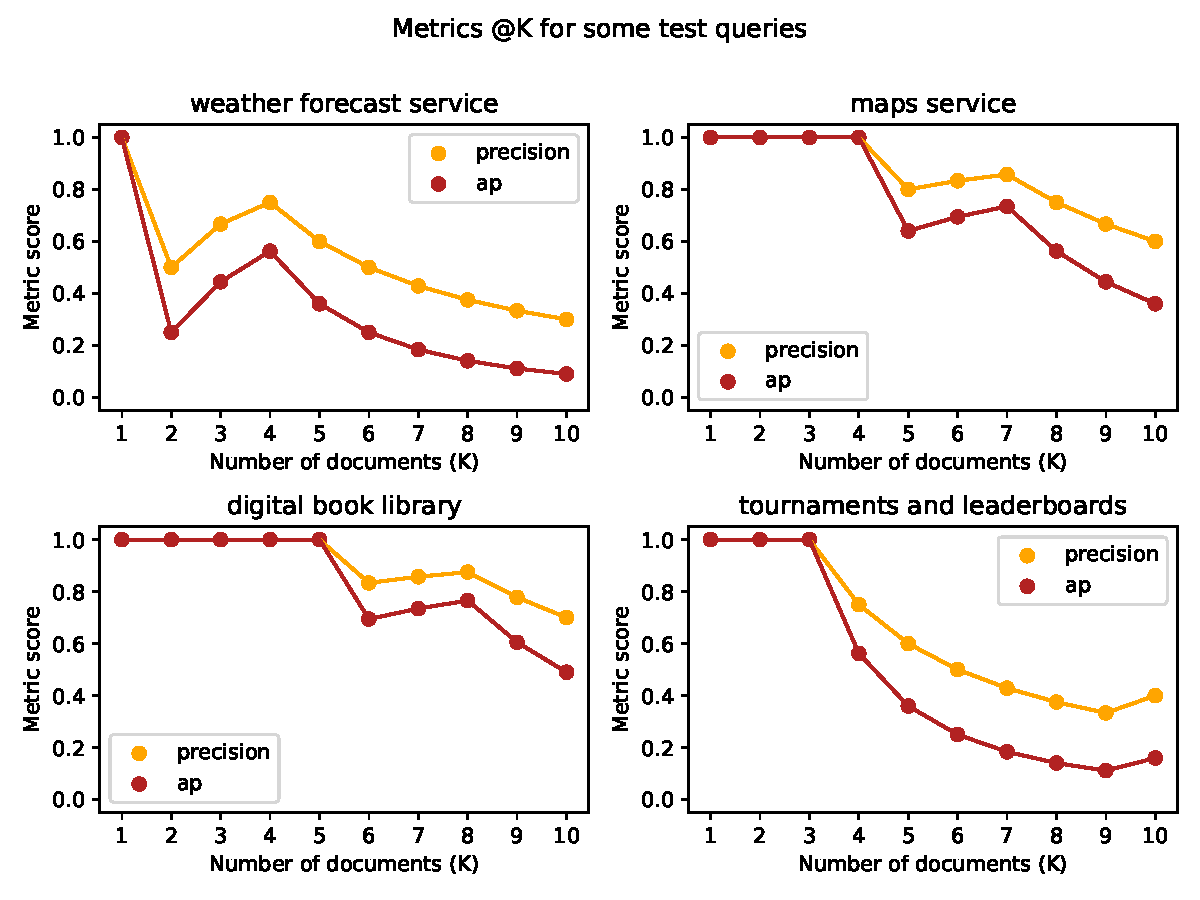
\includegraphics[width=0.8\linewidth]{assets/pdf/evaluation/ap}
    \end{center}

    \caption{Precision and Average Precision (AP)}
    \label{fig:ap}
\end{figure}

\begin{figure}[!h]
    \begin{center}
        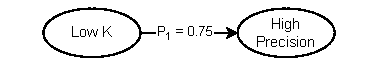
\includegraphics[width=0.4\linewidth]{assets/pdf/evaluation/dag-prec}
    \end{center}

    \caption{Causal graph with probabilities}
    \label{fig:dag-prec}
\end{figure}

\begin{figure}[!h]
    \begin{center}
        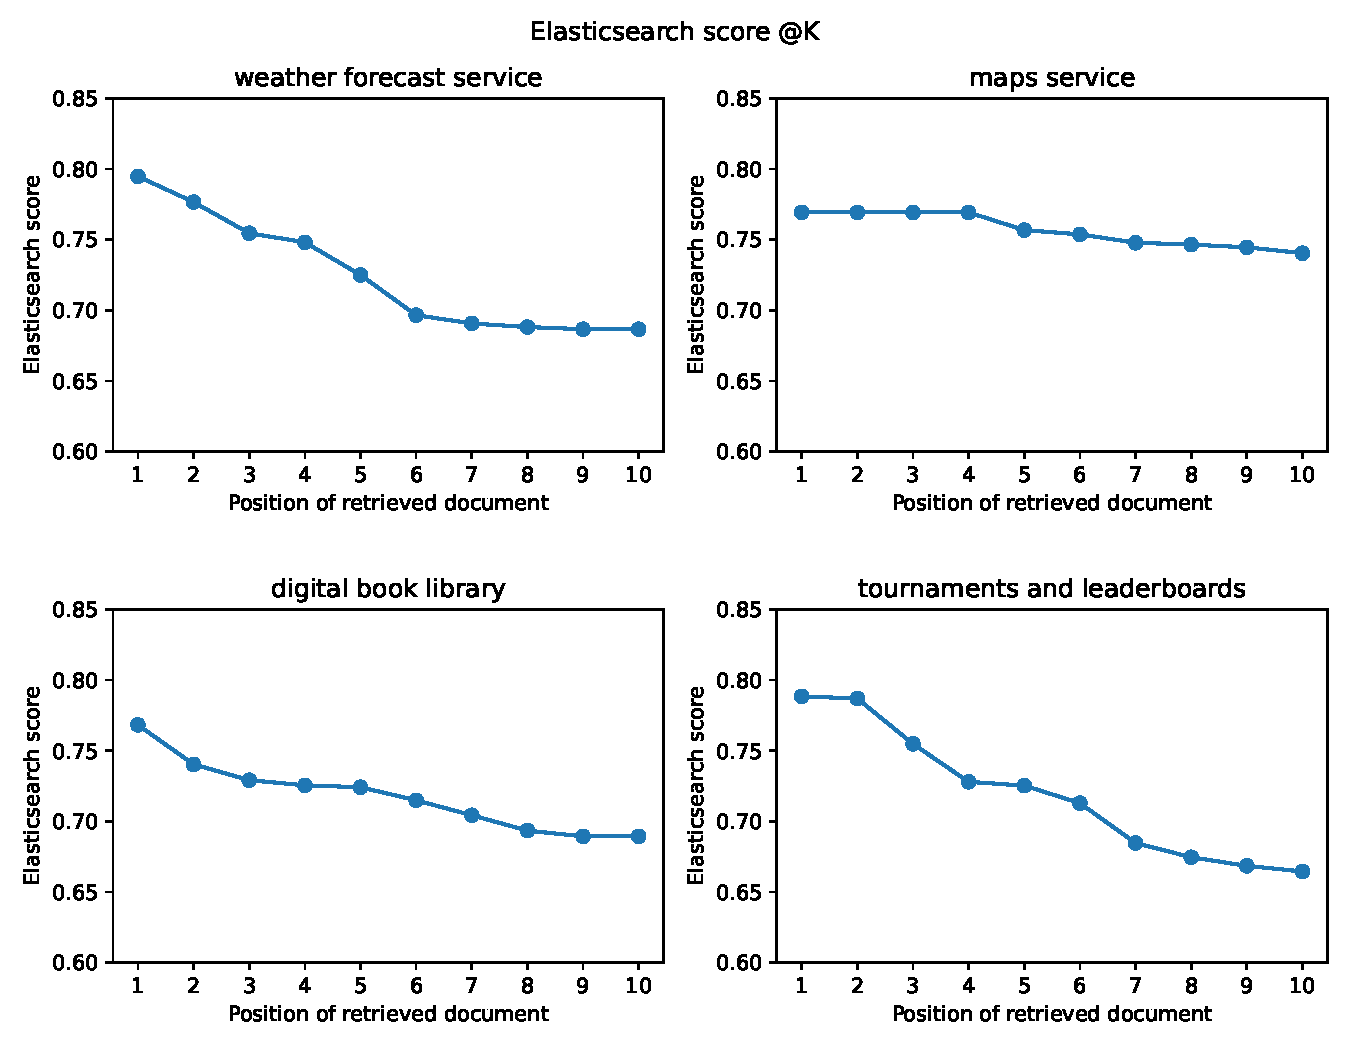
\includegraphics[width=0.8\linewidth]{assets/pdf/evaluation/es-scores}
    \end{center}

    \caption{Elasticsearch score for each retrieved document}
    \label{fig:es-scores}
\end{figure}

\section{Time Performance}\label{sec:time-performance}
In addition to experiments measuring the performance of our system, we also wanted to test its retrieval speed.
The speed was measured in two different scenarios.
In the first scenario, we do not insert any query, thus making the system send a non-KNN query to elastic (Section~\ref{subsec:api-scout-dsl-to-elasticsearch-search-dsl}).
In the second case, we insert a random three-word query (words were generated by an API \footnote{https://random-word-api.herokuapp.com/
}) for each iteration of the experiment.
In addition, in both scenarios, we ran each step 10 times, and with this data, we also computed the standard error for each step.\\ \\
The experiment was run for both scenarios for 12 different values of $K$ -- from 10 to 120 with a step of 10 documents.
Each time, we increased the size of the returned page by 10.
In the case of the first scenario, only the \verb|size| parameter was modified -- since it's not a KNN query.
On the other hand, when running the tests for the second scenario, we also increased the value of the \verb|k| parameter for each step.
Moreover, in the case of the second scenario, for each of the ten repetitions of a step, we generated -- as we said previously -- three words to be used as a query for the approximate KNN search.
This was done in order to try and force Elasticsearch to always perform a search from scratch, not using any cached data from previous search queries. \\ \\
For each scenario, we compute the retrieval time for each combination of fields.
Since we can filter for the \verb|metadata| and \verb|specification| fields, we tested the times for only metadata, only specification, and both metadata and specification.
The obtained graph can be seen in Figure~\ref{fig:time}.
Tables~\ref{tab:times-no-queries} and~\ref{tab:times-queries} displays all the mean retrieval times -- in milliseconds -- at each $@K$ for the \("\)no queries\("\) and \("\)random queries\("\) experiments.
From the two graphs, we can see that in the case of the \("\)no queries\("\) experiment, the retrieval times seem to plateau when we go over the 90 documents per page.
On the other side, in the \("\)random queries\("\), we see more of a linear increase in retrieval times over time.

\begin{figure}[!h]
    \begin{center}
        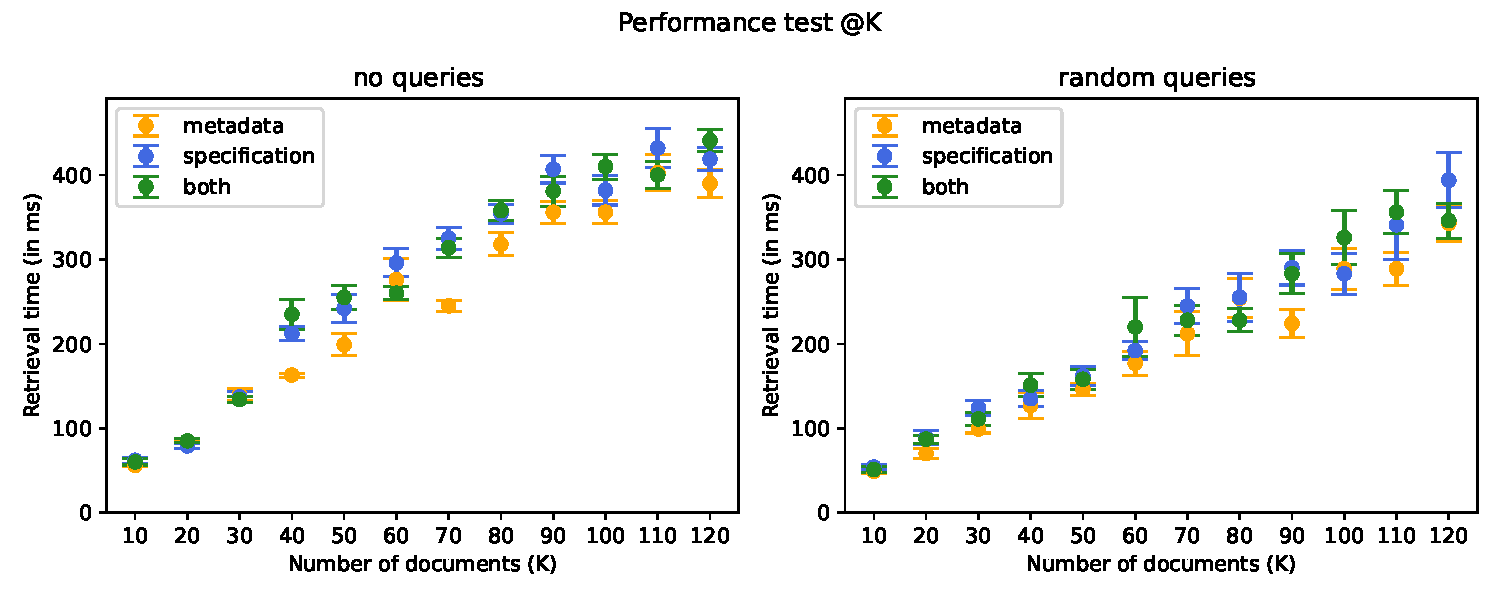
\includegraphics[width=0.8\linewidth]{assets/pdf/evaluation/time}
    \end{center}

    \caption{Retrieval times in milliseconds. Bars indicate the standard error}
    \label{fig:time}
\end{figure}

\begin{table}[!h]
    \begin{center}
        \begin{tabular}{l c c c c c c c c c c c c}
            \hline
            \textbf{Field} & \textbf{@10} & \textbf{@20} & \textbf{@30} & \textbf{@40} & \textbf{@50} & \textbf{@60} & \textbf{@70} & \textbf{@80} & \textbf{@90} & \textbf{@100} & \textbf{@110} & \textbf{@120} \\ \hline
            Metadata & 56 & 80 & 140 & 163 & 199 & 276 & 245 & 318 & 356 & 356 & 403 & 390 \\
            Specification & 62 & 79 & 137 & 212 & 242 & 296 & 325 & 354 & 407 & 382 & 432 & 419 \\
            Both & 60 & 85 & 134 & 235 & 255 & 260 & 314 & 358 & 381 & 410 & 400 & 441 \\ \hline \hline
            Mean & 59.3 & 81.3 & 137 & 203.3 & 232 & 277.3 & 294.6 & 343.3 & 381.3 & 382.6 & 411.6 & 416.6 \\ \hline
        \end{tabular}
    \end{center}

    \caption{Retrieval times in milliseconds for the "no queries" experiment}
    \label{tab:times-no-queries}
\end{table}

\begin{table}[!h]
    \begin{center}
        \begin{tabular}{l c c c c c c c c c c c c}
            \hline
            \textbf{Field} & \textbf{@10} & \textbf{@20} & \textbf{@30} & \textbf{@40} & \textbf{@50} & \textbf{@60} & \textbf{@70} & \textbf{@80} & \textbf{@90} & \textbf{@100} & \textbf{@110} & \textbf{@120} \\ \hline
            Metadata & 49 & 70 & 99 & 127 & 146 & 177 & 212 & 254 & 224 & 289 & 289 & 343 \\
            Specification & 54 & 89 & 124 & 135 & 162 & 192 & 245 & 255 & 290 & 283 & 341 & 394 \\
            Both & 51 & 87 & 111 & 151 & 158 & 220 & 228 & 228 & 283 & 326 & 356 & 346 \\ \hline \hline
            Mean & 51.3 & 82.0 & 111.3 & 137.6 & 155.3 & 196.3 & 228.3 & 245.6 & 265.6 & 299.3 & 328.6 & 361 \\ \hline
        \end{tabular}
    \end{center}

    \caption{Mean retrieval times in milliseconds for the "random queries" experiment}
    \label{tab:times-queries}
\end{table}

\noindent Let's now create a causal graph for this batch of experiments.
The graph will be composed of several nodes: \("\)Only Metadata\("\), \("\)Only Specification\("\), \("\)Both\("\), \("\)Random Queries\("\), \("\)No Queries\("\) and \("\)Faster Fetch Time\("\).
The \("\)Only Metadata\("\), \("\)Only Specification\("\), and \("\)Both\("\) nodes means that we only take into account the retrieval times of queries containing those fields.
The \("\)Random Queries\("\) and \("\)No Queries\("\) nodes mean that we only take into account the mean retrieval times of the queries in one experiment or the other.
Finally, the \("\)Faster Fetch Time\("\) nodes means that the mean retrieval time $@K$ coming from another node is lower than the retrieval time $@K$ coming from their alternative(s).
To clarify this last point, let's take into account the path Only Metadata $\rightarrow$ Faster Fetch Time.
In this case, we have a faster fetch time if the mean coming from the \("\)Only Metadata\("\) node is lower than both the \("\)specification\("\) and \("\)both\("\) means (that are found in Tables~\ref{tab:times-no-queries} and~\ref{tab:times-queries}). \\ \\
Now, we compute the probabilities all paths.
For the paths Only Metadata $\rightarrow$ Faster Fetch Time, Only Specification $\rightarrow$ Faster Fetch Time, and Both $\rightarrow$ Faster Fetch Time the probabilities will be:
\[P_1 = \frac{19}{24} = 0.8~~~~~~~~~~~~~~~P_2 = \frac{2}{24} = 0.1~~~~~~~~~~~~~~~P_3 = \frac{3}{24} = 0.1\]
While the probability for the paths Random Queries $\rightarrow$ Faster Fetch Time and No Queries $\rightarrow$ Faster Fetch Time will be:
\[P_4 = \frac{11}{12} = 0.9~~~~~~~~~~~~~~~P_5 = \frac{1}{12} = 0.1\]
The causal graphs are displayed in Figures~\ref{fig:dag-tmp-metadata} and~\ref{fig:dag-tmp-random}.
The final causal graph can be found in Figure~\ref{fig:dag-retrieval}.
This shows that there is a very high probability that, if we either filter for metadata or perform a search request using a query, we will have faster retrieval times.

\begin{figure}[!h]
    \begin{minipage}{0.48\textwidth}
        \centering
        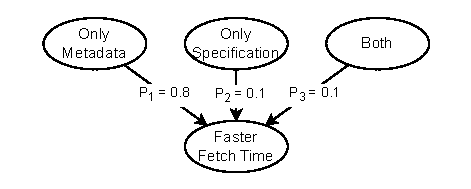
\includegraphics[width=0.9\linewidth]{assets/pdf/evaluation/dag-tmp-meta}
        \caption{Causal graph with probabilities}
        \label{fig:dag-tmp-metadata}
    \end{minipage}\hfill
    \begin{minipage}{0.48\textwidth}
        \centering
        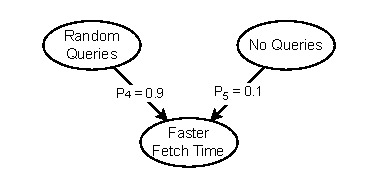
\includegraphics[width=0.8\linewidth]{assets/pdf/evaluation/dag-tmp-random}
        \caption{Causal graph with probabilities}
        \label{fig:dag-tmp-random}
    \end{minipage}

    \label{fig:dag-comparison}
\end{figure}

\begin{figure}[!h]
    \begin{center}
        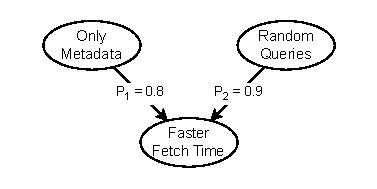
\includegraphics[width=0.4\linewidth]{assets/pdf/evaluation/dag-retrieval}
    \end{center}

    \caption{Causal graph with probabilities}
    \label{fig:dag-retrieval}
\end{figure}

\section{Summary and Outlook}\label{sec:summary-and-outlook-1}
In this section, we have shown and discussed some experiments that were performed on API Scout.
As we have seen, the system is almost always able to retrieve all the generated specifications within the first 10 results.
Moreover, the system seems to perform well overall, where the first retrieved documents are mostly relevant to the given query.
Finally, the retrieval speed increases linearly over time, and selecting only the \("\)metadata\("\) field leads to faster retrieval times overall.
In the next chapter, we will give some concluding remarks on the project and suggest some possible enhancements that could be implemented into API Scout in the future.



    %%%%%%%%%%%%%%%%%%%%%%%%%%%%%%%%%%%%%%%%%%%%%%%%%%%%%%%%%%%%%%%%%
    %%%	CONCLUSION %%%%%%%%%%%%%%%%%%%%%%%%%%%%%%%%%%%%%%%%%%%%%%%%%%
    %%%%%%%%%%%%%%%%%%%%%%%%%%%%%%%%%%%%%%%%%%%%%%%%%%%%%%%%%%%%%%%%%

    \chapter{Conclusion}\label{ch:conclusion}
This thesis set out with the objective of developing a tool -- API Scout -- that could help both academics and developers to better understand and analyze the evolution and structure of OpenAPI Specifications.
This chapter reflects on the entire research and development process, summarizing its key components, methodologies, and findings.
In addition, we will also be discussing the lessons learned, as well as potential areas for future enhancement.

\section{Retrospective}\label{sec:retrospective}
The main objective of this thesis was to create a tool which could efficiently embed, index, and retrieve OpenAPI Specifications.
In addition to this, we also wanted the user to be able to further refine their search by applying specific filters.
For this reason, we have also implemented an intuitive yet powerful filtering DSL\@. \\ \\
Below, we are going to have a look at all the sections that compose this thesis.

\begin{description}
    \item \textbf{Background} In the first part of this thesis, we started the research process by looking at existing research and methodologies.
    During this research process, we found several algorithms and methodologies that could have helped us reach our initial goal.
    Moreover, we also looked at the existing literature to see if someone had already laid the foundations upon which we could build our tool.
    \item \textbf{Experimentation} Following the study of the literature, we decided to create some proofs-of-concept to have a better understanding of the feasibility of our tool.
    In particular, we created a proof-of-concept for the embedding and indexing part of the tool.
    The evaluation of this method was done on a much smaller dataset (\textasciitilde 3'000 documents).
    \item \textbf{Methodology} After having developed a working and promising proof-of-concept, we started working on the actual implementation of the tool.
    We started by describing the grammar, operations, types, and parameters of the DSL\@.
    After, we defined the architecture of the system, and how all the different parts would be connected to create the final system.
    Finally, we talked about the actual implementation details of our system.
    \item \textbf{Evaluation} Being done with the implementation part, we started the evaluation process.
    Here, we employed different techniques and evaluation metrics to have a better understanding of the performance of our system.
    In particular, we tested both the accuracy -- i.e.\ how well it performed in retrieving relevant documents -- and speed -- i.e.\ in how many milliseconds the system retrieved the documents -- of the system.
\end{description}

\section{Lessons Learned}\label{sec:lessons-learned}
Throughout the course of this thesis, we have learned several key lessons that can also be applied in the future to improve our system.

\begin{description}
    \item \textbf{Have a standardized way of representing and saving data.} This has been crucial in our case since we were dealing with data scraped on different occasions, by different people, and from different sources.
    This helped us especially when building the database mapping for Elasticsearch and the DSL\@.
    \item \textbf{Employ scalable algorithms for embedding, indexing, and retrieving.} Since this tool needs to be accessed by possibly multiple users at the same time, it is of paramount importance to use efficient and scalable algorithms that can perform the indexing of the query and the retrieval of the documents in just a few milliseconds.
    Moreover, as the database grows, the algorithms must be able to handle and search into such a massive database.
    \item \textbf{Defining a solid ground truth and metrics before the evaluation process.} This was one of the major issues we had in the evaluation part of our proof-of-concept.
    We defined a ground truth that made some assumptions that could easily be wrong or inaccurate.
    For this reason, we re-built our ground truth -- and more in general our evaluation framework -- when evaluating the finished system.
    \item \textbf{Evaluate different aspects of the system.} This helped us to have a clearer view of how our system performed overall.
\end{description}

\section{Future Work}\label{sec:future-work}
The findings of this thesis open up several different avenues for possible future developments.
Below we have listed a few of them that could be interesting to investigate and possibly develop.

\begin{description}
    \item \textbf{Implement an algorithm to compute metrics for new specifications.} For now, the metrics have been provided by the database from which have taken our OpenAPI Specifications.
    It would be very useful to have an algorithm that would compute all the necessary metrics for each of the specifications added by some user.
    This would also eliminate the need for users to insert the metrics when sending the specifications to our backend, thus being able to have documents with identical structures in our database.
    \item \textbf{Implement a UI to show the evolution of APIs in time.} Another possible improvement would be the implementation of a User Interface (UI), which could graphically display both the structure and the changes made in each version of an OpenAPI Specification.
    In this way, the users could be able to see the evolution of an API at a glance.
    \item \textbf{Evaluate against other state-of-the-art embedding methodologies.} We could compare our embedding strategy with other state-of-the-art methodologies.
    In this way, we could have a more in-depth view of how our system performs.
\end{description}

\section{Concluding Remarks}\label{sec:concluding-remarks}
As shown throughout this report, our embedding, indexing, and retrieval techniques seems to be working well for several different queries.
Moreover, the filtering DSL is a great way of creating curated datasets of OpenAPI Specifications that could be used in a research setting.
Finally, all the aforementioned lessons learned and future works lay a strong foundation for the further improvement of the tool such that it can be more useful to the end users.



%%%%%%%%%%%%%%%%%%%%%%%%%%%%%%%%%%%%%%%%%%%%%%%%%%%%%%%%%%%%%%%%%
%%%	BIBLIOGRAPHY %%%%%%%%%%%%%%%%%%%%%%%%%%%%%%%%%%%%%%%%%%%%%%%%
%%%%%%%%%%%%%%%%%%%%%%%%%%%%%%%%%%%%%%%%%%%%%%%%%%%%%%%%%%%%%%%%%

    \newpage
    \bibliographystyle{ieeetr}
    \bibliography{bibliography/biblio}
\end{document}